\pdfoutput=1
\documentclass[letterpaper,11pt]{article}
\usepackage[margin=1in]{geometry}
\usepackage[CJKbookmarks=true,
            bookmarksnumbered=true,
            bookmarksopen=true,
            colorlinks=true,
            citecolor=red,
            linkcolor=blue,
            anchorcolor=red,
            urlcolor=blue
            ]{hyperref}
\usepackage[title]{appendix}
\usepackage{graphicx}
\usepackage{caption}
\usepackage{subcaption}
\usepackage{booktabs}
\usepackage{algorithm}
\usepackage{algorithmic}
\usepackage{amsmath,amsthm,amsfonts,amssymb}
\usepackage{hyperref}
\usepackage{color}
\usepackage{enumitem}
\usepackage{bm}
\usepackage{multirow}
\usepackage{bbm}
\usepackage{subfiles}
\usepackage{xspace}
\usepackage{mathtools} 
\usepackage{tikz}
\usepackage{natbib}
\newtheorem{condition}{Condition}
\newtheorem{theorem}{Theorem}
\newtheorem*{theorem*}{Theorem}
\newtheorem{lemma}{Lemma}
\newtheorem{corollary}{Corollary}

\newtheorem{problem}{Problem}
\newtheorem{assumption}{Assumption}
\newtheorem{proposition}{Proposition}

\theoremstyle{definition}
\newtheorem{remark}{Remark}
\newtheorem{definition}{Definition}

\providecommand{\keywords}[1]
{
  \small	
  \textbf{\textit{Keywords---}} #1
}


\newcommand{\arrowIn}{
\tikz \draw[-stealth] (-1pt,0) -- (1pt,0);
}
\newcommand{\arrowOut}{
\tikz \draw[-stealth] (1pt,0) -- (-1pt,0);
}
\tikzset{global scale/.style={
    scale=#1,
    every node/.append style={scale=#1}
  }
}
\newcommand{\gaussianrho}{\mathcal{N}\pth{\begin{pmatrix} 0 \\ 0 \end{pmatrix}, \begin{pmatrix} 1 & \rho \\ \rho & 1 \end{pmatrix}}}

\newcommand{\maA}{\mathcal{A}}
\newcommand{\maB}{\mathcal{B}}
\newcommand{\maC}{\mathcal{C}}
\newcommand{\maD}{\mathcal{D}}
\newcommand{\maE}{\mathcal{E}}
\newcommand{\maF}{\mathcal{F}}
\newcommand{\maG}{\mathcal{G}}
\newcommand{\maH}{\mathcal{H}}
\newcommand{\maI}{\mathcal{I}}
\newcommand{\maJ}{\mathcal{J}}
\newcommand{\maK}{\mathcal{K}}
\newcommand{\maL}{\mathcal{L}}
\newcommand{\maM}{\mathcal{M}}
\newcommand{\maN}{\mathcal{N}}
\newcommand{\maO}{\mathcal{O}}
\newcommand{\maP}{\mathcal{P}}
\newcommand{\maQ}{\mathcal{Q}}
\newcommand{\maR}{\mathcal{R}}
\newcommand{\maS}{\mathcal{S}}
\newcommand{\maT}{\mathcal{T}}
\newcommand{\maU}{\mathcal{U}}
\newcommand{\maV}{\mathcal{V}}
\newcommand{\maW}{\mathcal{W}}
\newcommand{\maX}{\mathcal{X}}
\newcommand{\maY}{\mathcal{Y}}
\newcommand{\maZ}{\mathcal{Z}}


\newcommand{\prob}[1]{ \mathbb{P}\left[ #1 \right] }
\newcommand{\expect}[1]{ \mathbb{E}\left[ #1 \right] }

\newcommand{\tb}{\binom}


\newcommand\CC{\textcolor{blue}}
\newcommand\CCC{\textcolor{red}}
\newcommand{\nb}[1]{{\sf\color{blue}[#1]}}
\newcommand{\nbr}[1]{{\sf\color{red}[#1]}}
\newcommand{\nbp}[1]{{\sf\color{purple}[#1]}}
\newcommand{\remarkhd}[1]{{\sf\color{magenta}[#1]}}

\newcommand{\reals}{\mathbb{R}}
\newcommand{\naturals}{\mathbb{N}}
\newcommand{\integers}{\mathbb{Z}}
\newcommand{\complex}{\mathbb{C}}

\newcommand{\ones}{\mathbbm{1}}
\newcommand{\zeros}{\mathbbm{0}}

\newcommand{\termI}{\mathrm{(I)}}
\newcommand{\termII}{\mathrm{(II)}}
\newcommand{\termIII}{\mathrm{(III)}}
\newcommand{\termIV}{\mathrm{(IV)}}

\newcommand{\en}{\mathsf{{e}}}
\newcommand{\vn}{\mathsf{{v}}}

\newcommand{\pth}[1]{\left( #1 \right)}
\newcommand{\qth}[1]{\left[ #1 \right]}
\newcommand{\sth}[1]{\left\{ #1 \right\}}

\newcommand{\calA}{{\mathcal{A}}}
\newcommand{\calB}{{\mathcal{B}}}
\newcommand{\calC}{{\mathcal{C}}}
\newcommand{\calD}{{\mathcal{D}}}
\newcommand{\calE}{{\mathcal{E}}}
\newcommand{\calF}{{\mathcal{F}}}
\newcommand{\calG}{{\mathcal{G}}}
\newcommand{\calH}{{\mathcal{H}}}
\newcommand{\calI}{{\mathcal{I}}}
\newcommand{\calJ}{{\mathcal{J}}}
\newcommand{\calK}{{\mathcal{K}}}
\newcommand{\calL}{{\mathcal{L}}}
\newcommand{\calM}{{\mathcal{M}}}
\newcommand{\calN}{{\mathcal{N}}}
\newcommand{\calO}{{\mathcal{O}}}
\newcommand{\calP}{{\mathcal{P}}}
\newcommand{\calQ}{{\mathcal{Q}}}
\newcommand{\calR}{{\mathcal{R}}}
\newcommand{\calS}{{\mathcal{S}}}
\newcommand{\calT}{{\mathcal{T}}}
\newcommand{\calU}{{\mathcal{U}}}
\newcommand{\calV}{{\mathcal{V}}}
\newcommand{\calW}{{\mathcal{W}}}
\newcommand{\calX}{{\mathcal{X}}}
\newcommand{\calY}{{\mathcal{Y}}}
\newcommand{\calZ}{{\mathcal{Z}}}

\newcommand{\ti}{\tilde}
\newcommand{\TV}{\mathsf{TV}}
\newcommand{\Bin}{\mathrm{Bin}}
\newcommand{\Bernoulli}{\mathrm{Bernoulli}}
\newcommand{\corr}{\mathrm{Corr}}
\newcommand{\overlap}{\mathrm{overlap}}
\newcommand{\supp}{\mathrm{Supp}}

\newcommand{\sfA}{{\mathsf{A}}}
\newcommand{\sfB}{{\mathsf{B}}}
\newcommand{\sfC}{{\mathsf{C}}}
\newcommand{\sfD}{{\mathsf{D}}}
\newcommand{\sfE}{{\mathsf{E}}}
\newcommand{\sfF}{{\mathsf{F}}}
\newcommand{\sfG}{{\mathsf{G}}}
\newcommand{\sfH}{{\mathsf{H}}}
\newcommand{\sfI}{{\mathsf{I}}}
\newcommand{\sfJ}{{\mathsf{J}}}
\newcommand{\sfK}{{\mathsf{K}}}
\newcommand{\sfL}{{\mathsf{L}}}
\newcommand{\sfM}{{\mathsf{M}}}
\newcommand{\sfN}{{\mathsf{N}}}
\newcommand{\sfO}{{\mathsf{O}}}
\newcommand{\sfP}{{\mathsf{P}}}
\newcommand{\sfQ}{{\mathsf{Q}}}
\newcommand{\sfR}{{\mathsf{R}}}
\newcommand{\sfS}{{\mathsf{S}}}
\newcommand{\sfT}{{\mathsf{T}}}
\newcommand{\sfU}{{\mathsf{U}}}
\newcommand{\sfV}{{\mathsf{V}}}
\newcommand{\sfW}{{\mathsf{W}}}
\newcommand{\sfX}{{\mathsf{X}}}
\newcommand{\sfY}{{\mathsf{Y}}}
\newcommand{\sfZ}{{\mathsf{Z}}}

\newcommand{\sfa}{{\mathsf{a}}}
\newcommand{\sfb}{{\mathsf{b}}}
\newcommand{\sfc}{{\mathsf{c}}}
\newcommand{\sfd}{{\mathsf{d}}}
\newcommand{\sfe}{{\mathsf{e}}}
\newcommand{\sff}{{\mathsf{f}}}
\newcommand{\sfg}{{\mathsf{g}}}
\newcommand{\sfh}{{\mathsf{h}}}
\newcommand{\sfi}{{\mathsf{i}}}
\newcommand{\sfj}{{\mathsf{j}}}
\newcommand{\sfk}{{\mathsf{k}}}
\newcommand{\sfl}{{\mathsf{l}}}
\newcommand{\sfm}{{\mathsf{m}}}
\newcommand{\sfn}{{\mathsf{n}}}
\newcommand{\sfo}{{\mathsf{o}}}
\newcommand{\sfp}{{\mathsf{p}}}
\newcommand{\sfq}{{\mathsf{q}}}
\newcommand{\sfr}{{\mathsf{r}}}
\newcommand{\sfs}{{\mathsf{s}}}
\newcommand{\sft}{{\mathsf{t}}}
\newcommand{\sfu}{{\mathsf{u}}}
\newcommand{\sfv}{{\mathsf{v}}}
\newcommand{\sfw}{{\mathsf{w}}}
\newcommand{\sfx}{{\mathsf{x}}}
\newcommand{\sfy}{{\mathsf{y}}}
\newcommand{\sfz}{{\mathsf{z}}}

\newcommand{\tr}{\mathrm{Tr}}

\newcommand{\Binom}{\mathrm{Binomial}}
\newcommand{\Uniform}{\mathrm{Uniform}}
\newcommand{\norm}[1]{\left\|{#1} \right\|}
\newcommand{\Norm}[1]{\|{#1} \|}
\newcommand{\HG}{\mathrm{HG}}

\newcommand{\indc}[1]{{\mathbf{1}_{\left\{{#1}\right\}}}}
\newcommand{\Indc}{\mathbf{1}}

\newcommand{\ER}{Erd\H{o}s-R\'enyi }
\newcommand{\argmax}{\mathrm{argmax}}
\newcommand{\aut}{\mathsf{aut}}
\newcommand{\sub}{\mathsf{sub}}
\renewcommand{\hom}{\mathsf{hom}}
\newcommand{\inj}{\mathsf{inj}}
\newcommand{\vp}{\varphi}
\newcommand{\stophere}{\remarkhd{stop here}}

\def\var{\mathrm{Var}}
\def\E{\mathbb{E}}
\def\P{\mathbb{P}}

% ------------ tikz draw
\def\nodebullet{\node[fill=black,circle,inner sep=0pt,minimum size=3pt]}

\usepackage{xcolor}
\definecolor{red1}{RGB}{255, 0, 0}  
\definecolor{red2}{RGB}{220, 47, 2}   
\definecolor{red3}{RGB}{189, 58, 85}


\usetikzlibrary{intersections,calc,decorations.pathreplacing,through,arrows}
\usetikzlibrary{ decorations.markings,positioning}

\title{Testing Correlation in Graphs by Counting Bounded Degree Motifs}
%\author{}
\date{}
\author{Dong Huang and Pengkun Yang\thanks{D.\ Huang and P.\ Yang are with the Department of Statistics and Data Science, Tsinghua University. P. Yang is supported in part by National Key R\&D Program of China 2024YFA1015800, 
% National Natural Science Foundation of China (NSFC) Grant 12101353, 
Tsinghua University Dushi Program 2025Z11DSZ001, and High Performance Computing Center, Tsinghua University.}}


\begin{document}

\maketitle

\begin{abstract}
We investigate the problem of detecting correlation between two \ER graphs $\maG(n,p)$, formulated as a hypothesis testing problem: under the null hypothesis, the two graphs are independent, while under the alternative hypothesis, they are correlated through a latent bijective mapping between their vertex sets. We develop a polynomial-time test by counting bounded degree motifs and prove its effectiveness for any constant correlation coefficient $\rho$ when the edge connection probability satisfies $p\ge n^{-1+\delta}$ for some constant $\delta>0$. 
In particular, our guarantee improves the constrain of motif-counting methods from $\rho\ge\sqrt{\alpha}$ to any constant $\rho = \Omega(1)$, where $\alpha\approx 0.338$ is the Otter's constant.
   
   %Our results surpass the  limitation on Otter's constant for correlation $\rho$, extending it to any constant $\rho$ using a simple construction.
   %The algorithm runs in time $n^{(1/\rho)^C}$.
\end{abstract}

\begin{keywords}
    {Hypothesis testing, correlation detection, bounded degree motif, \ER graph, polynomial-time algorithm}
\end{keywords}

%\tableofcontents

\section{Introduction}\label{sec-intro}

Correlation analysis between datasets is one of the most fundamental problems in statistics. %This problem arises naturally in many domains, such as survival analysis~\citep{martin2005testing}, statistical genetics~\citep{liu2010versatile}, ecological risk assessment~\citep{dishion1999middle}, and independent component analysis~\citep{lu2009financial}. 
In the classical vector setting, the problem of testing independence between two random vectors has been extensively studied, including low-dimensional~\citep{pearson1900x,kendall1938new,spearman1987proof} and high-dimensional settings~\citep{szekely2007measuring,zhu2017projection,gretton2007kernel}.
%For low-dimensional vectors, commonly used measures of dependence include the Pearson's correlation~\citep{pearson1900x}, Kendall's tau~\citep{kendall1938new}, and Spearman's rho~\citep{spearman1987proof}. In the high-dimensional setting, the independence tests have been developed based on distance covariance~\citep{szekely2007measuring}, projection correlation~\citep{zhu2017projection}, the Hilbert-Schmidt independence criterion~\citep{gretton2007kernel}, rank of distances~\citep{heller2013consistent}, mutual information~\citep{berrett2019nonparametric}, among others. 
In contrast, correlation analysis for graph-structured data remains much less explored. 
Indeed, since shared randomness increases the overlap of network patterns across graphs, correlation often manifests as structural similarity between graphs, which is common in real scenarios.
Recently, there has been a surge of interest in the problem of analyzing correlated graphs, as in many applications the observations are more naturally represented as graphs rather than vectors. 
Such problems arise from various domains:
\begin{itemize}
    \item In social network analysis, whether two friendship networks on different social network platforms share structural similarities is a crucial task in privacy protection~\citep{narayanan2008robust}.%,narayanan2009anonymizing}.
    \item In computer vision, 3-D shapes can be represented as graphs, and a significant problem is determining whether two graphs represent the same object under deformations~\citep{berg2005shape}.%,mateus2008articulated}.
    \item In natural language processing, one important problem is the ontology alignment problem, which refers to uncovering the correlation between two different knowledge graphs~\citep{haghighi2005robust}.%,hughes2007lexical}.
    \item In computational biology, proteins can be regarded as vertices and the interactions between them can be formulated as weighted edges, and the protein-protein interactions (PPI) can be represented as a graph~\citep{singh2008global}.%,vogelstein2015fast}.
\end{itemize}

A common strategy for handling graph data is through graph embedding. Among such approaches, spectral embedding is a widely used method that maps graphs into low-dimensional vectors~\citep{rohe2011spectral}. % and offers theoretical guarantees under random graph models~\citep{sussman2013consistent}. 
This strategy has been applied to testing independence between graphs~\citep{lee2019network} and to defining measures of graph correlation~\citep{fujita2017correlation}.
Despite its popularity, spectral embedding has several limitations. First, it requires selecting an embedding dimension which is often heuristic and lacks theoretical guarantees. Second, reducing graphs to vector representations inevitably sacrifices structural information compared with analyzing graphs directly. Third, spectral embedding relies on singular value decomposition, which can be computationally prohibitive for large-scale networks.
These challenges highlight the need for correlation measures that operate directly on graph topology while remaining both statistically sound and computationally efficient. Motivated by this gap, we aim to develop a new method for testing correlation between two graphs.
%A common strategy for handling the graph data is through graph embedding strategy. Spectral embedding is one choice, which transfers graph data to low-dimensional vectors~\cite{rohe2011spectral} and can be proven to have theoretical guarantee under random graph models~\citep{sussman2013consistent,rubin2022statistical}. This method has been used in testing the independence between two graphs~\citep{lee2019network} and as a measure of graph correlation~\citep{fujita2017correlation}. However, the spectral embedding strategy has certain limitations: 1) spectral embedding requires a selection of embedding dimensions, which is typically estimated by graph data and can be inaccurate; 2) there is a lose of information by analyzing the resulting vectors than directly analyzing the original graph data; and 3) spectral embedding can be slow because of the use of singular value decomposition.  Therefore, it is natural to wonder if there exists a proper correlation measure that can be used directly between two graphs which can be computed fast.

%In this paper, we aim to provide a graph correlation testing method to quantify the association between two graphs.

Building on the hypothesis testing framework proposed in~\cite{barak2019nearly}, for two graphs $G_1,G_2$ with vertex sets $V(G_1),V(G_2)$ and edge sets $E(G_1), E(G_2)$,
we consider the following graph correlation detection problem: under the null hypothesis $\maH_0$, $G_1$ and $G_2$ are independent; under the alternative hypothesis $\maH_1$, there exists a latent vertex bijection $\pi:V(G_1)\mapsto V(G_2)$ that induces correlation between the edges of the two graphs. 
Specifically, for any $uv\in E(G_1)$ with $u,v\in V(G_1)$, the corresponding pair $\pi(u)\pi(v)$ lies in $E(G_2)$, and the edges $uv$ and $\pi(u)\pi(v)$ are statistically correlated.
Under both \(\maH_0\) and \(\maH_1\), each graph marginally follows the same random-graph model; what distinguishes \(\maH_1\) is the presence of statistical dependence between corresponding edges across the two graphs.
%\nbr{You may elaborate a bit for general graph model (without ER), and then move Section 1.1 to the theory section. It seems the key is on the model of correlation. The marginal random graph models sounds non-essential in the introduction. }
Given $G_1$ and $G_2$, the goal is to test $\maH_0$ against $\maH_1$ by the latent structure
under $\maH_1$. 

In this paper, we focus on the \ER model~\cite{paul1959random}.
Specifically, the \ER random graph $\maG(n,p)$ is the graph on $n$ vertices where each edge connects with probability $0<p<1$ independently. %While there are differences between the \ER random graph model and the networks derived from real-world scenarios, comprehensively understands the \ER graphs remains profoundly significant, as it serves as a pivotal step in transitioning from solving problems from \ER graphs to addressing challenges in practical applications \nbr{this statement sounds unclear}.
Under the null hypothesis $\maH_0$, the two graphs $G_1$ and $G_2$ follow $\maG(n,p)$ independently; under the alternative hypothesis $\maH_1$, $G_1$ and $G_2$ follow the following \emph{correlated \ER graph} $\maG(n,p,\rho)$.
\begin{definition}[Correlated \ER graph]
    For two random graphs $G_1,G_2$ with vertex sets $V(G_1),V(G_2)$ and edge sets $E(G_1),E(G_2)$, let $\pi$ denote a latent bijective mapping from $V(G_1)$ to $V(G_2)$. We say $(G_1,G_2)$ follows \emph{correlated \ER graph} $\maG(n,p,\rho)$ if both marginal distributions are \ER graph $\maG(n,p)$ and each pair of edges $(uv,\pi(u)\pi(v))$ follows the correlated bivariate Bernoulli distribution with correlation coefficient $\rho$ for any $u,v\in V(G_1)$.
\end{definition}

%In this work, we focus on the special case where $G_1$ and $G_2$ follow \ER graph distribution $\maG(n,p)$. Specifically, the \ER random graph is the graph on $n$ vertices where each edge connects with probability $0<p<1$ independently. Under the null hypothesis $\maH_0$, $G_1$ and $G_2$ follow independent \ER model $\maG(n,p)$; under the alternative hypothesis $\maH_1$, $G_1$ and $G_2$ follow the following \emph{correlated \ER graph} $\maG(n,p,\rho)$.
%\begin{definition}[Correlated \ER graph]
%    For two random graphs $G_1,G_2$ with vertex sets $V(G_1),V(G_2)$ and edge sets $E(G_1),E(G_2)$, let $\pi$ denote a latent bijective mapping from $V(G_1)$ to $V(G_2)$. We say $(G_1,G_2)$ follows \emph{correlated \ER graph} $\maG(n,p,\rho)$ if both marginal distributions are \ER graph $\maG(n,p)$ and each pair of edges $(uv,\pi(u)\pi(v))$ follows the correlated bivariate Bernoulli distribution with correlation coefficient $\rho$ for any $u,v\in V(G_1)$.
%\end{definition}

%\nbr{$\calP_0$ and $\calP_1$?}
Let $\maP_0$ and $\maP_1$ denote the probability measures for $(G_1,G_2)$ under $\maH_0$ and $\maH_1$, respectively. We say a test statistic $\maT(G_1,G_2)$ with a threshold $\tau$ succeeds in detection, if the sum of Type I and Type II errors is bounded by $0.05$ as $n\to \infty$:
\begin{align}\label{eq:detection-cretiria}
    \limsup_{n\to \infty}\qth{\maP_0(\maT\ge\tau)+\maP_1(\maT< \tau)}\le 0.05.
\end{align}
%\nbr{I don't think $c$ is a common notation for error probability}
%\remarkhd{$\TV$ remove; add correlation detection in vec/matrix(graph property, challenge in graph structure, and practical influence) --> hardness in our problem}
%
%\remarkhd{more literature in section 1, rewrite related work}
%
%\remarkhd{computation cost (to sell the method)}
%
%\remarkhd{Trade-off between statistical efficiency (?) and computation cost}
%
%\remarkhd{Faster algorithm (iterative algorithm for the motif family)}
%
In fact, the detection threshold can be improved from $0.05$ to any prescribed positive constant; see Remark~\ref{rmk:005} for details.
It is well-known that the minimal value of the sum of Type I and Type II errors between $\maP_0$ and $\maP_1$ is achieved by the likelihood ratio test (see, e.g., \cite[Theorem 13.1.1]{lehmann2005testing}). %In order to analyze the information-theoretic threshold for correlation detection, it is equivalent to analyze the total variation distance $\TV(\maP,{\maP_0})$. %A problem related to correlation detection in random graphs is the graph matching problem, which refers to finding a node correspondence that maximizes the edge correlation given a pair of correlated graphs~\citep{conte2004thirty}. 
However, the likelihood ratio test requires the evaluation over the space of latent permutations incurring a computational cost of $n!$.
In order to design scalable tests, one must instead exploit informative graph properties that can be computed efficiently while still being identifiable for the underlying models. 
One common and significant methodology is to look at the graphs from a motif perspective, identifying the characteristic and recurrent connection patterns.
%Indeed, several previous works have adopted motif counting for correlation analysis and network analysis. For example, method-of-moments estimators based on empirical subgraph counts give consistent procedures and asymptotic theory for graph-moment statistics~\citep{bickel2011method}. In a similar spirit, subgraph-based two-sample and distributional-equivalence tests have been developed and validated on real networks~\citep{ghoshdastidar2020two}. 
For correlation detection between two graphs, \cite{barak2019nearly} analyzed counts of balanced graphs (denser than any of their subgraphs), whereas \cite{mao2024testing} used tree counts to obtain detection guarantees. Both approaches aggregate over large motif families, reflecting that usable correlation signal accumulates with the family size.

Despite their theoretical appeal, balanced graphs or tree structures rarely occur in real-world settings such as social networks.
A line of research instead focuses on counting other types of motifs. %including triads~\citep{schank2005finding}, cliques~\citep{finocchi2015clique}, stars~\citep{gonen2011counting}, and subtrees~\citep{li2018mtmo}.
However, relying on a single class of motifs often yields weak signals and can significantly limit performance.
Thus, the central challenge is to design test statistics that are not only powerful and computationally efficient, but also flexible to capture the structural characteristics of real networks.

In this paper, we introduce a new approach based on counting bounded degree motifs, namely motifs whose vertex degrees are bounded by a universal constant. This family is broad—encompassing balanced graphs, trees, triads, cliques, and stars—and therefore provides richer structural information.
% , leading to stronger detection signals and well-behaved estimators under standard graph models.
Importantly, it includes commonly observed patterns such as triangles and quadrilaterals, which frequently appear in real-world networks.
Moreover, we establish rigorous theoretical guarantees for the bounded degree motif family, showing that it offers both statistical power and practical relevance.
In addition, bounded degree motifs can be efficiently estimated even on large networks: they admit scalable counting via local exploration or graph sampling techniques, thereby avoiding exhaustive enumeration over all subgraphs.
%\nbr{May briefly mention somewhere: another computational benefit on large networks is that motifs can be estimated by graph sampling; moreover, bounded degree motifs can be counted efficiently using local exploration techniques, avoiding the need for exhaustive searches. }

\subsection{Main Results}

In this subsection, we present the main results. 

\begin{theorem}\label{thm:main}
Assume that $p\ge n^{-1+\delta}$ for some constant $\delta>0$. Then for any constant correlation $\rho=\Omega(1)$, there exists a polynomial-time computable test statistic $\maT$ and a threshold $\tau$ such that
\[
\limsup_{n\to\infty}\big[\maP_0(\maT\ge \tau)+\maP_1(\maT<\tau)\big]\le 0.05.
\]
\end{theorem}

We will show in Section~\ref{sec:general-motif} that any \emph{$C$-admissible} motif family is sufficient for detection.  In Section~\ref{sec:bd-sub-count}, we prove that when $p\ge n^{-2/3}$ and $\rho=\Omega(1)$, there exists a \emph{$C$-admissible} motif family by constructing a bounded degree motif family.  In Section~\ref{sec:refined-results}, we further develop a refined bounded degree construction that is sufficient for detection under the weaker condition $p\ge n^{-1+\delta}$ and $\rho=\Omega(1)$, thereby establishing Theorem~\ref{thm:main}.

It is shown in~\cite{barak2019nearly} that a polynomial-time algorithm based on counting balanced graphs succeeds for correlation detection when $p\in [n^{-1+\epsilon},n^{-1+1/153}]\cup [n^{-1/3},n^{-\epsilon}]$ for any sufficiently small constant $\epsilon>0$ and $\rho=\Omega(1)$, where a balanced graph is denser than each of its nontrivial subgraphs. The recent work~\cite{mao2024testing} proposed a polynomial-time algorithm based on counting trees, which succeeds in detection when $p\ge n^{-1+o(1)}$ and $\rho^2\ge \alpha\approx 0.338$, where $\alpha$ is Otter's constant~\cite{otter1948number}. In view of Theorem~\ref{thm:main}, our test succeeds over the broad range $p\ge n^{-1+\delta}$ for any constant $\rho=\Omega(1)$ by counting bounded degree motifs.%, thereby overcoming the limitation imposed by Otter's constant and achieving detection for all constant correlations.

For the remaining regimes,~\cite{ding2023low} provided evidence from the low-degree framework that the condition $\rho^2\ge \alpha$ is essential for detection when $p=n^{-1+o(1)}$. When $p\le n^{-1-\delta}$ for some constant $\delta>0$, detection is information-theoretically impossible~\cite{wu2023testing,ding2023detection}. Taken together, these results suggest that Theorem~\ref{thm:main} attains the strongest detection guarantee achievable by polynomial time. We note that~\cite{ding2023polynomial} also provided a polynomial-time matching algorithm (based on a nontrivial iterative procedure) that works when $p\ge n^{-1+\delta}$ and $\rho=\Omega(1)$, and hence can be adapted to detection. In contrast, our approach achieves the same detection regime via a simple and natural motif counting statistic, avoiding the more intricate iterative procedure.

Following~\cite{ding2023low,li2025algorithmic} and motivated by the low-degree framework~\cite{hopkins2018statistical}, there is evidence that any degree-$o(\rho^{-1})$ polynomial fails for detection in the \ER model. Consequently, when $\rho=o(1)$, no constant-degree polynomial is expected to succeed. This suggests that our assumption $\rho=\Omega(1)$ is essentially necessary for polynomial-time algorithms within this framework. 
%In summary, existing polynomial-time algorithms and corresponding computational hardness results are essentially optimal outside the regime $p\ge n^{-1+\delta}$, while in the regime $p\ge n^{-1+\delta}$ our guarantees are suggested to be rate-optimal.



\subsection{Test Statistics}\label{sec:method}

To obtain a computationally efficient test, a natural approach is to use summary statistics rather than searching over all possible bijective mappings. 
% \nbr{start from identifiability considerations}
Ideally, the graph can be uniquely identified from a sufficiently rich set of summary statistics. 
% A statistic that captures graph properties is a promising choice, as it exhibits greater similarity under the correlated model than under the independent model. 
Graph homomorphism numbers provide a particularly prominent class of such statistics. 
% is one of such estimators. 
Specifically, for two simple graphs $\sfM$ and $G$,
% with vertex sets $V(\sfM),V(G)$ and edge sets $E(\sfM),E(G)$, 
a homomorphism of $\sfM$ into $G$ is an edge-preserving mapping from $V(\sfM)$ to $V(G)$. Let $\hom(\sfM,G)$ be the number of homomorphisms of $\sfM$ into $G$.  
It is well-known that the function of homomorphism numbers $\hom(\cdot,G)$ uniquely determines a simple graph $G$ (see, e.g., \cite[Theorem 5.29]{lovasz2012large}). By~\cite{muller1977edge}, when $\en(G)\ge \vn(G)\log \vn(G)$, the homomorphism numbers $\hom(\sfM,G)$ for motifs $\sfM$ with $\en(\sfM)<\en(G)$ determine $G$. It is further conjectured that $\hom(\sfM,G)$ for all $\vn(\sfM)<V(G)$ or $\en(\sfM)<\en(G)$ determine $G$ if $\vn(G)\ge 3$ and $\en(G)\ge 4$ \cite[Conjectures 5.30 and  5.31]{lovasz2012large}.
However, computing $\hom(\sfM,G)$ for all $\sfM$ up to the scale of $G$ is still computationally prohibitive. 
We instead consider the number of injective homomorphisms of $\sfM$ into $G$ denoted by $\inj(\sfM,G)$, which can be applied to evaluate $\hom(\sfM,G)$ \cite[(5.16)]{lovasz2012large}.
% a closely related quantity $\inj(\sfM,G)$ that denotes the number of injective homomorphisms of $\sfM$ into $G$ that can be used to evaluate $\hom(\sfM,G)$ \cite[(5.16)]{lovasz2012large}.
% Then $\hom(\sfM,G)$ can be evaluated via the summation of $\inj(\sfM/P,G)$ over all partitions of $\vn(\sfM)$, where $\sfM/P$ denotes the simple quotient graph by merging each class of $P$ into a single node.  
% Let $\inj(\sfM,G)$ be the number of injective homomorphisms of $\sfM$ into $G$.
Indeed, $\inj(\sfM,G)$ indicates the motif counts of $\sfM$ in $G$. 
We only compute a subset of injective homomorphism numbers over an informative family of motifs $\sfM\in \calM$. 



In our correlation detection problem, given a motif $\sfM$, the injective homomorphism numbers $\inj(\sfM,G_1)$ and $\inj(\sfM,G_2)$ are independent under the null hypothesis $\maH_0$, while they are correlated under the alternative $\maH_1$. 
The quantity $$\pth{\inj(\sfM,G_1)-\expect{\inj(\sfM,G_1)}}\pth{\inj(\sfM,G_2)-\expect{\inj(\sfM,G_2)}}$$ indicates the correlation between $\inj(\sfM,G_1)$ and $\inj(\sfM,G_2)$, which serves as a basis for distinguishing $\maH_0$ from $\maH_1$.
Naturally, the definition of homomorphism numbers can be extended to the case where $G$ is a weighted graph associated with vertex set $V(G)$ and weighted edge set $\sth{\beta_{uv}(G):u,v\in V(G)}$. For any mapping $\varphi:V(\sfM)\mapsto V(G)$, we define $\hom_\varphi(\sfM,G) = \prod_{uv\in E(\sfM)}\beta_{\varphi(u)\varphi(v)}(G)$ and \begin{align}\label{eq:def_of_inj}
    % \hom(\sfM,G) = \sum_{\varphi:V(\sfM)\mapsto V(G)} \hom_\varphi(\sfM,G),\quad 
    \inj(\sfM,G) = \sum_{\substack{\varphi:V(\sfM)\mapsto V(G)\\\varphi\text{ injective}}} \hom_\varphi(\sfM,G).
\end{align}



Given a graph $G$, we first center the weights and obtain a weighted graph $\bar{G}$ with weighted edges 
% For an \ER graph $G\sim \maG(n,p)$ with vertex set $V(G)$ and edge set $E(G)$, let $\bar{G}$ denote the weighted graph with same vertex and edge sets, and the weight associated with each edge is defined as 
$\beta_{uv}(\bar{G}) = \indc{uv\in E(G)} - \expect{\indc{uv\in E(G)}}$ for $u,v\in V(G)$, where $\expect{\indc{uv\in E(G)}}$ can be estimated by the average degree of the graph. 
% Although all of the homomorphism numbers $\hom(\cdot, \bar{G}_1)$ and $\hom(\cdot,\bar{G}_2)$ determine the graph $\bar{G}_1 $ and $\bar{G}_2$, it is intractable to compute in practice.
% As a practical alternative,  we consider computing the injective homomorphism number in a motif family, which is also equivalent to computing such motif counts in two graphs.
Then, for a given motif family $\maM$, our test statistic is defined as \begin{align}\label{eq:est-sub-count}
    \maT_{\maM }\pth{G_1,G_2} = \sum_{\sfM \in \maM } \omega_\sfM\, \inj(\sfM,\bar{G}_1)\inj(\sfM,\bar{G}_2),
\end{align}
where $\omega_\sfM$ is a weight function to be specified.
% of $\sfM,n,p$, and $\rho$, which will be introduced later. 
This test statistic can be interpreted as an inner product between the two vectors $\qth{\inj(\sfM,\bar{G}_1)}_{\sfM\in \maM}$ and $\qth{\inj(\sfM,\bar{G}_2)}_{\sfM\in \maM}$. 
% While these vectors encode structural properties of the graphs, their inner product quantifies the correlation between the two graphs. 
By picking an appropriate threshold $\tau$, we define the test that rejects the null hypothesis $\maH_0$ whenever $\maT_\maM(G_1,G_2)\ge \tau$. We will theoretically analyze the resulting Type I and Type II errors in Section~\ref{sec:general-motif}.

%we will theoretically analyze the Type I and Type II errors of the test statistics $\maT_\maM(G_1,G_2)$\nbr{explicitly say when to reject null}.
% together with the motif counting estimator $\maT_\maM(G_1,G_2)$, we will show that the sum of Type I and Type II errors is bounded away from a small error under certain conditions.


A richer motif family captures more graph properties and can strengthen the effectiveness of the test at a higher computational cost. 
% Indeed, the testing error can be further reduced by counting more comprehensive structures.
Our motif-counting statistic has a computational cost at most $O(n^{\en(\maM)})$, where $\en(\maM)\triangleq\max_{\sfM\in \maM}\en(\sfM)$ is the maximum number of edges among motifs in the family $\maM$.
Our theory requires $\en(\maM)\ge f(0.05)$ for some function $f$ to achieve a prescribed error probability $0.05$; see Sections~\ref{sec:general-motif},~\ref{sec:bd-sub-count} and~\ref{sec:refined-results} for further details. This setting illustrates a fundamental trade-off between statistical accuracy and computational efficiency: as $\en(\maM)\to\infty$, the sum of Type I and Type II errors vanishes, but at the expense of an increasing runtime of $O(n^{\en(\maM)})$.


The previous work~\cite{mao2024testing} adopted the motif counting statistic with the tree motifs and showed that detection is possible when the correlation coefficient is beyond some constant under the \ER random graph model. %, which is defined as the graph that is denser than its subgraphs. They propose a polynomial algorithm when $\rho  =\Omega(1)$ and edge connection density $p\in [n^{-1+\epsilon},n^{-1+1/153}]\cup [n^{-1/3},n^{-\epsilon}]$ for any constant $0<\epsilon <1$. Another related  work~\cite{mao2024testing} counts the trees with fixed edges and succeeds for detection when the correlation coefficient satisftying $\rho^2>\alpha$, where $\alpha$ is the Otter's constant introduced in~\cite{otter1948number}. 
%However, there is a close connection between \ER graph and Poisson-Galton-Watson tree.
%Indeed, the local structure of sparse \ER graph is asymptotically distributed as Galton-Watson tree (see, e.g.~\cite{ganassali2024statistical}).
The effectiveness of tree counting statistics relies significantly on the tree-like substructures inherent in the graph model.
As a result, such statistics may become less effective for graph models or datasets that lack a tree-like structure,
% In real-world network data, tree structures often disappear, 
raising the natural question of whether we can count more general motifs.
In this paper, we consider bounded degree motifs that are commonly observed in practice. Let $\maM(N_\sfe,d)$ denote the set of all connected bounded degree motifs with $N_\sfe$ edges and maximum degree bounded by $d$. For example, 
\[\maM_{3,2} = \sth{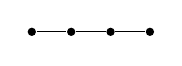
\begin{tikzpicture}[scale=0.5, baseline={([yshift=-.5ex]current bounding box.center)}]
    \nodebullet  (a) at (0,0) {};
    \nodebullet (b) at (1,0) {};
    \nodebullet (c) at (2,0) {};
    \nodebullet (d) at (3,0) {};
    \draw (a) -- (b) -- (c) -- (d);
\end{tikzpicture}\,,\quad 
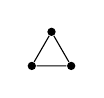
\begin{tikzpicture}[scale=0.5, baseline={([yshift=-.5ex]current bounding box.center)}]
    \nodebullet (b) at (0,0) {};
    \nodebullet (c) at (0.5,-0.866) {};
    \nodebullet (d) at (-0.5,-0.866) {};
    \draw (c) -- (d) -- (b) -- (c);
\end{tikzpicture}
},\quad 
\maM_{4,3} = \left\{ 
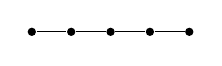
\begin{tikzpicture}[scale=0.5, baseline={([yshift=-.5ex]current bounding box.center)}]
    \nodebullet  (a) at (0,0) {};
    \nodebullet (b) at (1,0) {};
    \nodebullet (c) at (2,0) {};
    \nodebullet (d) at (3,0) {};
    \nodebullet (e) at (4,0) {};
    \draw (a) -- (b) -- (c) -- (d) -- (e);
\end{tikzpicture}\, ,
\quad
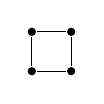
\begin{tikzpicture}[scale=0.5, baseline={([yshift=-.5ex]current bounding box.center)}]
    \nodebullet (a) at (0,0) {};
    \nodebullet (b) at (1,0) {};
    \nodebullet (c) at (1,1) {};
    \nodebullet (d) at (0,1) {};
    \draw (a) -- (b) -- (c) -- (d) -- (a);
\end{tikzpicture}\, ,
\quad
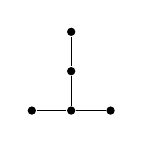
\begin{tikzpicture}[scale=0.5, baseline={([yshift=-.5ex]current bounding box.center)}]
    \nodebullet (a) at (0,0) {};
    \nodebullet (b) at (1,0) {};
    \nodebullet (c) at (2,0) {};
    \nodebullet (e) at (1,1) {};
    \nodebullet (f) at (1,2) {};
    \draw (a) -- (b) -- (c);
    \draw (b) -- (e);
    \draw (e) -- (f);
\end{tikzpicture}\, ,\quad 
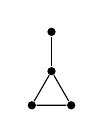
\begin{tikzpicture}[scale=0.5, baseline={([yshift=-.5ex]current bounding box.center)}]
    \nodebullet (a) at (0,1) {};
    \nodebullet (b) at (0,0) {};
    \nodebullet (c) at (0.5,-0.866) {};
    \nodebullet (d) at (-0.5,-0.866) {};
    \draw (c) -- (d) -- (b) -- (c);
    \draw (b) -- (a);
\end{tikzpicture}
\right\}.
\]
While the bounded degree counting test statistic $\maT_{\maM(N_\sfe,d)}$  remains valid for detection, we will consider two subsets of bounded degree motifs $\maM(N_\sfv,N_\sfe,d),\overline{\maM}(N_\sfv,N_\sfe,d)\subseteq \maM(N_\sfe,d)$ that are more simplified and easier to analyze. See Sections~\ref{sec:bd-sub-count} and~\ref{sec:refined-results} for further details. Indeed, our approach unifies and generalizes several existing motif counting methods: \cite{barak2019nearly} counted balanced graphs, \cite{mao2024testing} counted trees, and \cite{jin2025counting} counted cycles. By counting all bounded degree motifs, our statistic subsumes these as special cases and captures a richer range of structural correlations.
%\nbr{Add somewhere on the connection and difference from other motif counting method like cycle count statistics. Better not miss relevant literature within statistics community.}
\subsection{Related Work}

%\emph{Polynomial-time algorithm.} It is shown in~\cite{barak2019nearly} that a polynomial-time algorithm based on counting balanced graphs succeeds in the correlation detection when $p\in [n^{-1+\epsilon},n^{-1+1/153}]\cup [n^{-1/3},n^{-\epsilon}]$ for any small constant $\epsilon>0$ and $\rho$ is a constant, where a balanced graph refers to a graph that is denser than its subgraphs. The recent work~\cite{mao2024testing} proposed a polynomial-time algorithm based on counting trees, which succeeds in detection when $p\ge n^{-1+o(1)}$ and $\rho^2>\alpha\approx 0.338$, where $\alpha$ is the Otter's constant introduced in~\cite{otter1948number}.

\emph{Polynomial-time algorithms and computational hardness.}
It was shown in~\cite{barak2019nearly} that counting balanced subgraphs succeeds in detecting correlation in correlated \ER graphs for any constant $\rho$, provided that the edge probability $p$ lies in a suitable regime. Extending this line of work,~\cite{mao2024testing} demonstrated that counting trees achieves successful correlation detection over a broader range of $p$, as long as $\rho$ exceeds a fixed constant.
From the computational-hardness perspective, the low-degree conjecture—motivated by the sum-of-squares framework—is widely believed to offer a unifying approach to predicting computational lower bounds in a broad class of high-dimensional statistical problems~\citep{hopkins2017efficient,hopkins2018statistical,schramm2022computational,sohn2025sharp}. This conjecture has yielded tight hardness predictions for many problems, including graph matching, planted clique, planted dense subgraph, community detection, tensor PCA, and sparse PCA~\citep{hopkins2017efficient,hopkins2017power,hopkins2018statistical,bandeira2019computational,schramm2022computational,ding2023low,kunisky2024tensor,dhawan2025detection,li2025algorithmic}. %Moreover, fixing a constant degree $d$, if the signal-to-noise ratio is $1+o(1)$ for all polynomials $f$ of degree at most $d$, then this suggests that polynomial-based algorithms of degree below $d$ cannot distinguish $\maP_1$ from $\maP_0$. Building on this conjecture, \cite{ding2023low,li2025algorithmic} provided evidence that any degree-$o(\rho^{-1})$ polynomial algorithm fails for detection.

\emph{Information-theoretic analysis.}
\cite{wu2023testing} characterized a sharp detection threshold—at which the optimal testing error exhibits a phase transition—by analyzing the maximum likelihood test for dense correlated \ER graphs with edge probability $p=n^{-o(1)}$. For sparse graphs with $p=n^{-\Omega(1)}$, they also derived the threshold up to constant factors. Building on this, \cite{ding2023detection} further sharpened the sparse-graph threshold via an analysis of the densest subgraphs. More recently, \cite{huang2025sample,huang2026information} investigated correlation detection for induced subgraphs under the Gaussian Wigner model and the \ER model.

\emph{Graph matching.}
Closely related to correlation detection is the graph matching problem, which seeks a node correspondence maximizing the edge agreement (or edge correlation) between a pair of correlated graphs~\citep{conte2004thirty}. A variety of polynomial-time algorithms have been proposed, including approaches based on subgraph counting~\citep{mao2025random,maier2025asymmetric}, neighborhood statistics~\citep{dai2019analysis,ding2021efficient,mao2021random}, spectral methods~\citep{umeyama1988eigendecomposition,singh2008global,fan2019spectral,ganassali2022spectral}, convex relaxations~\citep{aflalo2015convex,vogelstein2015fast,varma2025graph}, greedy algorithms~\citep{du2025algorithmic}, and iterative refinements~\citep{piccioli2022aligning,ding2023polynomial,ganassali2024statistical}. From an information-theoretic viewpoint, sharp thresholds and phase transitions for exact and partial recovery, along with impossibility regimes, have been investigated in a series of works~\citep{cullina2016improved,cullina2017exact,cullina2020partial,ganassali2020tree,ganassali2021impossibility,wu2022settling,ding2023matching,du2025optimal,hall2023partial}.

\subsection{Notation and Paper Organization}

For any $n\in \mathbb{N}$, let $[n]\triangleq \{1,2,\cdots,n\}$. 
We use standard asymptotic notation: for two positive sequences $\{a_n\}$ and $\{b_n\}$, we write $a_n = O(b_n)$ or $a_n\lesssim b_n$, if $a_n\le C b_n$ for some absolute constant $C$ and all $n$; $a_n = \Omega(b_n)$ or $a_n\gtrsim b_n$, if $b_n = O(a_n)$; $a_n = \Theta(b_n)$ or $a_n\asymp b_n$, if $a_n = O(b_n)$ and $a_n = \Omega(b_n)$; $a_n = o(b_n)$ or $b_n =\omega(a_n)$, if $a_n/b_n\to 0$ as $n\to \infty$.
Let $[x]$ denote the greatest integer less than or equal to $x$.

For a given weighted graph $G$, let $V(G)$ denote its vertex set and $E(G)$ its edge set. 
We write $uv$ to represent an edge $\{u,v\}$, and $\beta_{e}(G)$ for the weight of the edge $e$. 
 For an unweighted graph $G$, we define $\beta_{uv}(G)=\indc{uv\in E(G)}$.
Let $\vn(G)=|V(G)|$ denote the number of vertices in $G$, and $\en(G)=\sum_{e\in E(G)} \beta_{e}(G)$ the total weight of its edges. For any bijective mapping $\pi:V(G_1)\mapsto V(G_2)$, we define  $\pi(uv) = \pi(u)\pi(v)$ for any $u,v\in V(G_1)$. For simplicity, we write $\pi(e)$ to denote $\pi(uv)$ for any edge $e =uv$.
We write $\sfH_1 = \sfH_2$ if and only if they are isomorphic, that is, there exists a bijection $\pi:V(\sfH_1)\mapsto V(\sfH_2)$ such that $uv\in E(\sfH_1)$ if and only if $\pi(u)\pi(v)\in E(\sfH_2)$.
For any bijective mapping $\pi: V(G_1)\mapsto V(G_2)$ and subgraph $\sfH\subseteq G_1$, we define $\pi(\sfH)$ as the graph with\begin{align}\label{eq:def-piH}
    E(\pi(\sfH)) = \sth{\pi(u)\pi(v):uv\in E(\sfH)},V(\pi(\sfH)) = \sth{\pi(v):v\in V(\sfH)}.
\end{align}
For two graphs $G$ and $G'$, let $G\cap G'$ denote the graph with\begin{align}\label{eq:intersec-graph}
    E(G\cap G') = E(G)\cap E(G'), V(G\cap G') = \sth{v\in V(G)\cup V(G'):\exists u, uv\in E(G\cap G')}.
\end{align}
Let $G\cup G'$ denote the graph with
\begin{align}\label{eq:union-graph}
    E(G\cup G') = E(G)\cup E(G'),V(G\cup G') = V(G)\cup V(G').
\end{align}
Let $G\triangle G'$ denote the graph with 
\begin{align}\label{eq:triangle-graph}
    E(G\triangle G') = E(G)\triangle E(G'), V(G\triangle G') = \sth{v\in V(G)\cup V(G'):\exists u, uv\in E(G\triangle G')}.
\end{align}
The intersection $G \cap G'$ represents the subgraph consisting of all edges shared by $G$ and $G'$, along with the vertices incident to those edges.
The symmetric difference $G \triangle G'$ represents the subgraph containing edges that appear in exactly one of $G$ or $G'$. Moreover, we have \begin{align*}
    |V(G\triangle G')| = \vn(G)+\vn(G')-2|V(G)\cap V(G')|+|V(G\triangle G')\cap (V(G)\cap V(G'))|.
\end{align*} 

 


%\section{Additional Numerical Results}\label{apd:experiment}  

%\subsection{Synthetic Data}\label{apdsec:syn-data}



%\subsection{Real Data}

The remainder of the paper is organized as follows. 
%Section~\ref{sec:method} presents our methodology. 
In Section~\ref{sec:general-motif}, we establish theoretical guarantees for the proposed
statistics under general conditions.
Section~\ref{sec:bd-sub-count} introduces a specific motif family and shows
that the corresponding statistic performs well on graph models.
In Section~\ref{sec:refined-results}, we extend the condition $p\ge n^{-2/3}$ to the sparser regime $p\ge n^{-1+\delta}$ by counting a more delicate class of motifs.
In Section~\ref{sec:num-results}, we provide simulation studies. We finish in Section~\ref{sec:discussion}. Some technical proofs are deferred to the Appendices.






% In order to test $\maH_0$ against $\maH_1$, a natural approach is the likelihood ratio test. %In particular, the maximum likelihood estimator (MLE) is obtained by maximizing the overlap over all bijective mappings $\pi:V(G_1)\mapsto V(G_2)$:\begin{align*}
 %\underset{\pi:V(G_1)\mapsto V(G_2)}{\max}\sum_{u,v\in V(G_1)}\indc{uv\in E(G_1)}\indc{\pi(u)\pi(v)\in E(G_2)}.
%\end{align*}
% However, computing the MLE requires evaluating all $n!$ possible bijective mappings, which is computationally intractable. Since we only observe two unlabeled graphs, any valid test must rely on the graph properties that are invariant under graph isomorphisms, such as motif counting methods~\citep{barak2019nearly, mao2024testing} and spectral methods~\citep{fan2019spectral}.
%In this paper, we consider the bounded degree motif counting statistics, which counts the number of bounded degree motifs in two graphs.



\section{General Motif Counting Statistic}\label{sec:general-motif}
%\nbr{another section title?}

% Numerous graph models exist, with the \ER model being a prominent example, as proposed by~\cite{paul1959random} and~\cite{gilbert1959random}.



In this section, we establish the basic properties for the motif counting statistic $\maT_\maM$ in~\eqref{eq:est-sub-count} under the \ER model for general motif family $\maM$. To achieve the detection criterion~\eqref{eq:detection-cretiria}, it is crucial to select an appropriate motif family $\maM$. To this end, we will show that, by choosing appropriate weights $\omega_\sfM$ in $\maT_\maM$,
\[
\E_{\maP_1}\!\left[\maT_\maM\right] = \var_{\maP_0}\!\left[\maT_\maM\right] = \sum_{\sfM\in \maM}\rho^{2\en(\sfM)}.
\]
Since $\E_{\maP_0}[\maT_\maM] = 0$, the signal-to-noise ratio of the test statistic is given by
\begin{align}\label{eq:signal-to-noise}
    \frac{\E_{\maP_1}[\maT_\maM]-\E_{\maP_0}[\maT_\maM]}{\sqrt{\var_{\maP_0}[\maT_\maM]}}
= \sqrt{\sum_{\sfM\in \maM}\rho^{2\en(\sfM)}}.
\end{align}
As a result, by choosing the threshold $\tau=\frac{1}{2}\E_{\maP_1}[\maT_\maM]$, the quantity $\sum_{\sfM\in \maM}\rho^{2\en(\sfM)}$ plays a key role in controlling the Type~I error $\maP_0(\maT_\maM\ge \tau)$ by Chebyshev's inequality:
\begin{align}\label{eq:Chebyshev}
    \maP_0(\maT_\maM\ge \tau)\le \frac{4\var_{\maP_0}(\maT_\maM)}{(\E_{\maP_1}[\maT_\maM])^2} = \frac{4}{\sum_{\sfM\in \maM}\rho^{2\en(\sfM)}}.
\end{align}
On the other hand, controlling the Type~II error requires bounding $\maP_1(\maT_\maM<\tau)$. By Chebyshev's inequality,
\begin{align}
    \maP_1(\maT_\maM<\tau)\le \maP_1\pth{|\maT_\maM-\E_{\maP_1}[\maT_\maM]|\ge \frac{1}{2}\E_{\maP_1}[\maT_\maM]}\le \frac{4\var_{\maP_1}(\maT_\maM)}{(\E_{\maP_1}[\maT_\maM])^2},
\end{align}
so it remains to control $\var_{\maP_1}(\maT_\maM)$. Specifically, we show that motif counting based on the following family is sufficient for detection.

\begin{definition}\label{def:admissible}
We say that a motif family $\maM$ is \emph{$C$-admissible} if \begin{enumerate}
\item \label{cond:connect}For all $\sfM\in \maM$, $\sfM$ is connected;
    \item\label{cond:num} There exists $C=o\pth{\frac{\log n}{\max\pth{\log\log n,-\log\rho}}}$ such that $\vn(\sfM)\vee\en(\sfM)\le C$ for all $\sfM\in \maM$;
    \item\label{cond:signal-strength} $\sum_{\sfM\in \maM} \rho^{2\en(\sfM)}\ge 400$;
    \item\label{cond:subgraph} There exists a small constant $\epsilon_0$ such that, $n^{\vn(\sfM')} p^{\en(\sfM')}\ge n^{\epsilon_0}$ for all $\sfM\in \maM$ and subgraph $\emptyset\neq \sfM'\subseteq \sfM$. %\nbr{non-emtpy subgraph?}
\end{enumerate}
\end{definition}

Condition~\ref{cond:num} ensures that the size of each motif is bounded by $C$. Under this condition, the computation time of the statistic $\maT_\maM$ is $O(n^{C})$. 
Condition~\ref{cond:signal-strength} sets a lower bound on the overall signal strength, requiring that $\sum_{\sfM\in \maM} \rho^{2\en(\sfM)}\ge 400$. This requirement can be challenging to meet in practice: when the number of edges $\en(\sfM)$ grows, although $\maM$ contains more motifs, the term $\rho^{2\en(\sfM)}$ decreases quickly if $\rho$ is small. Consequently, one needs to balance the size $|\maM|$ and the quantity $\rho^{2\en(\sfM)}$ to ensure the family still carries enough signal.
Thus, Condition~\ref{cond:signal-strength} directly contributes to the Type~I error analysis.
Condition~\ref{cond:subgraph} is a technical requirement that ensures control of the variance $\var_{\maP_1}[\maT_\maM]$, which is essential for Type~II error analysis.
Intuitively, when a motif contains overly dense subgraphs, their occurrences become highly dependent, which inflates the variance $\var_{\maP_1}\!\left[\maT_\maM\right]$ and undermines the power of the test.
The requirement
\(
n^{\vn(\sfM')}\, p^{\en(\sfM')}\ge n^{\epsilon_0}
\)
ensures that each substructure appears with sufficient frequency to stabilize the test statistic, preventing such variance explosion.
This condition naturally motivates the use of bounded degree motifs, whose subgraphs are not excessively dense and thus allow for uniform variance control across the motif family.
The following theorem provides a theoretical guarantee for the counting statistic based on any \emph{$C$-admissible} motif family.


%The first condition indicates that the size of the motif is bounded by a universal constant $C$. Note that the non-isomorphic motifs with at most $C$ edges is bounded by constant, and counting the motifs with $C$ vertices in a graph with $n$ vertices needs a computation time of $O(n^{C})$. Therefore, the computation time of motif counting statistic $\maT_\maM$ is $O(n^{C})$ under the first condition. For the second condition, we will show that $\E_{\maP_1}\qth{\maT_\maM} = \var_{\maP_0}[\maT_\maM]=\sum_{\sfM\in \maM}\rho^{2\en(\sfM)}$ by picking appropriate weight $\omega_\sfM$ in $\maT_\maM$. Since $\E_{\maP_0}\qth{\maT_\maM} = 0$, the quantity $\frac{\E_{\maP_1}\qth{\maT_\maM}-\E_{\maP_0}[\maT_{\maM}]}{\sqrt{\var_{\maP_0}[\maT_\maM]}}=\sqrt{\sum_{\sfM\in \maM}\rho^{2\en(\sfM)}}$ reflects the signal-to-noise ratio for the test statistic. Consequently, the second condition contributes to significance analysis. The third condition is a technical condition for controlling the variance $\var_{\maP_1}\qth{\maT_\maM}$, which contributed to the power analysis. The following Theorem provides the theoretical guarantee for \emph{$c$-admissible} motif family counting statistic.

\begin{theorem}\label{thm:admissible}
    For any \emph{$C$-admissible} motif family $\maM$, there exist $\tau,\omega_\sfM\in \mathbb{R}$ such that,
    \begin{align*}
        \maP_0\pth{\maT_\maM\ge\tau}+\maP_1(\maT_\maM< \tau)\le 0.05.
    \end{align*}
\end{theorem}
%The proof of Theorem~\ref{thm:admissible} is deferred to Appendix~\ref{apd:proof-thm-admi}.
Theorem~\ref{thm:admissible} shows that the test statistic based on any \emph{$C$-admissible} motif family suffices for detection. In Section~\ref{sec:bd-sub-count}, we will construct a specific sub-family of bounded degree motifs $\maM'\subseteq \maM(N_\sfe,d)$ and prove that $\maM'$ is \emph{$C$-admissible}. Consequently, the statistic $\maT_{\maM'}$ achieves successful detection. In the following, we outline a general recipe for controlling the Type I and Type II errors on $\maT_\maM$.

\begin{remark}\label{rmk:005}
It follows from~\eqref{eq:signal-to-noise} and~\eqref{eq:Chebyshev} that the Type~I error can be made arbitrarily small provided that
$\sum_{\sfM\in\maM}\rho^{2\en(\sfM)}$ is sufficiently large.
For the Type~II error, Proposition~\ref{prop:admissible-TypeII} implies that it can also be made arbitrarily small.
In fact, for the constructions in Sections~\ref{sec:bd-sub-count} and~\ref{sec:refined-results}, Condition~\ref{cond:signal-strength} can be strengthened by replacing the constant $400$ with any prescribed constant (while keeping the same assumptions on $p$ and $\rho$), which in turn allows the target error level (e.g., $0.05$) to be replaced by any fixed constant.
Since the proof is identical up to constant changes, we omit the details.
\end{remark}


\subsection{Type I Error Control via Signal Score Estimation}

In this subsection, we show that the Type I error for the motif counting statistic with a \emph{$C$-admissible} motif family can be bounded by $O\pth{\frac{1}{\sum_{\sfM\in \maM} \rho^{2\en(\sfM)}}}$, where the quantity $\sum_{\sfM\in \maM} \rho^{2\en(\sfM)}$ is defined as the \emph{signal score} of the motif family, since it captures the strength of the signal-to-noise ratio. In order to distinguish $\maH_0$ from $\maH_1$ by the test statistic $\maT_\maM$, one natural choice for $\tau$ is to pick $\tau = \frac{1}{2}\pth{\E_{\maP_0}\qth{\maT_\maM}+\E_{\maP_1}\qth{\maT_\maM}}=\frac{1}{2}\E_{\maP_1}\qth{\maT_\maM}$. Applying Chebyshev's inequality yields the Type I error: \begin{align*}
    \maP_0\pth{\maT_\maM\ge \tau}\le \frac{\var_{\maP_0}\qth{\maT_\maM}}{\tau^2}=\frac{4\var_{\maP_0}\qth{\maT_\maM}}{\pth{\E_{\maP_1}\qth{\maT_\maM}}^2}.
\end{align*}
With appropriately chosen weights $\omega_\sfM$, we have $\var_{\maP_0}\qth{\maT_\maM} = \E_{\maP_1}\qth{\maT_\maM} =\sum_{\sfM\in \maM} \rho^{2\en(\sfM)}$. Therefore, the Type I error is bounded by $\frac{4}{\sum_{\sfM\in \maM} \rho^{2\en(\sfM)}}$. 
Let $\aut(\sfM)$ denote the number of automorphisms of $\sfM$.
In particular, we have the following proposition.
\begin{proposition}\label{prop:TypeI-admissible}
    For the statistic $\maT_\maM$ with weight $\omega_\sfM = \frac{\rho^{\en(\sfM)} (n-\vn(\sfM))!}{n! (p(1-p))^{\en(\sfM)}\aut(\sfM)}$, if $\tau = \frac{1}{2}\E_{\maP_1}\qth{\maT_\maM}$, then %\nbr{confirm $\omega_\sfM$? check throughout including main text, proofs, codes}
    \begin{align*}
        \maP_0\pth{\maT_\maM\ge \tau}\le \frac{4}{\sum_{\sfM\in \maM} \rho^{2\en(\sfM)}}.
    \end{align*}
\end{proposition}
The proof of Proposition~\ref{prop:TypeI-admissible} is deferred to Appendix~\ref{apd:proof-prop-admi-typeI}.
In view of Proposition~\ref{prop:TypeI-admissible}, the Type I error can be controlled as long as the \emph{signal score} is sufficiently large. 
If the motif family $\maM$ is \emph{$C$-admissible},
Condition~\ref{cond:signal-strength} in Definition~\ref{def:admissible} ensures that the Type I error is bounded by $0.01$. In practice, however, the parameters $p$ and $\rho$ may not be known a priori. A natural approach is to estimate these parameters from the observed graph data. While the edge probability $p$ can be reasonably approximated by the empirical edge density, estimating the correlation coefficient $\rho$ is substantially more challenging. To circumvent this challenge, we often restrict our attention to motif families satisfying
\[
\en(\sfM) = \en(\sfM') \quad \text{for all } \sfM,\sfM' \in \maM.
\]
Since all motifs in \(\mathcal M\) have the same number of edges, the factor $\rho^{\en(\sfM)}\,[p(1-p)]^{-\en(\sfM)}$
is constant across \(\sfM\in \maM\) and can be absorbed into a global normalization. Hence, instead of $\omega_{\sfM}=\frac{\rho^{\en(\sfM)}(n-\vn(\sfM))!}{n!(p(1-p))^{\en(\sfM)}\aut(\sfM)}$,
we may take the  choice $\omega_{\sfM}=\frac{(n-\vn(\sfM))!}{n!\aut(\sfM)}$.
With this choice, the statistic $\maT_\maM$ does not depend on the unknown correlation coefficient \(\rho\) (nor on \(p\) through the weights); the omitted constant is absorbed by the final normalization of the test.
%Instead of picking $\omega_\sfM = \frac{\rho^{\en(\sfM)}(n-\vn(\sfM))!\aut(\sfM)}{n!(p(1-p))^{\en(\sfM)}}$, we can pick $\omega_\sfM = \frac{(n-\vn(\sfM))!\aut(\sfM)}{n!}$ since the edges of motifs are equal among the family. By such new $\omega_\sfM$, our statistic does not rely on the correlation coefficient.
A concrete example of such a \emph{$C$-admissible} motif family with equal edge numbers will be presented in Section~\ref{sec:bd-sub-count}.
%In terms of Proposition~\ref{prop:TypeI-admissible}, the Type I error can be controlled provided that the \emph{signal score} is sufficiently strong. The second condition of a \emph{$C$-admissible} motif family guarantees that the Type I error is bounded by $\frac{c}{5}$. In practice, however, the parameters $p$ and $\rho$ may be unknown. A natural approach is to estimate these parameters from the observed graph data. While the edge probability $p$ can be approximated by the empirical edge density of the graph, estimating the correlation coefficient $\rho$ is substantially more challenging. To circumvent this difficulty, we typically restrict to motif families satisfying $\en(\sfM) = \en(\sfM')$ for all $\sfM,\sfM' \subseteq \maM$. A concrete example of such a \emph{$C$-admissible} motif family with equal edge numbers is presented in Section~\ref{sec:bd-sub-count}.




\subsection{Type II Error Control via Second Moment Analysis}

In this subsection, we establish the main results for controlling the Type II error. By Chebyshev's inequality, we obtain \begin{align*}
    \maP_1\pth{\maT_\maM<\tau} \le \maP_1\pth{\left| \maT_\maM-\E_{\maP_1}\qth{\maT_\maM}\right|>\tau}\le \frac{4\var_{\maP_1}\qth{\maT_\maM}}{\pth{\E_{\maP_1}\qth{\maT_\maM}}^2}.
\end{align*}
With a suitable choice of weights $\omega_\sfM$, we have already shown that $\E_{\maP_1}[\maT_\maM]$ is characterized by the \emph{signal score} $\sum_{\sfM\in \maM} \rho^{2\en(\sfM)}$. The remaining task is to control the variance, which requires estimating the second moment $\E_{\maP_1}[\maT_\maM^2]$. This analysis involves carefully handling the correlated terms under $\maP_1$, especially the off-diagonal terms in the second-moment expansion. Indeed, Condition~\ref{cond:subgraph} in the definition of a \emph{$C$-admissible} motif family is precisely designed to ensure such control. In particular, we obtain the following Proposition for controlling the Type II error.

\begin{proposition}\label{prop:admissible-TypeII}
    For motif counting statistic $\maT_\maM$ with \emph{$C$-admissible}  family $\maM$ and weight $\omega_\sfM = \frac{\rho^{\en(\sfM)}(n-\vn(\sfM))!}{n!(p(1-p))^{\en(\sfM)}\aut(\sfM)}$, if $\tau = \frac{1}{2}\E_{\maP_1}\qth{\maT_\maM}$, then \begin{align*}
        \maP_1\pth{\maT_\maM<\tau}\le 4\Bigg(3n^{-\epsilon_0/2}(4C)^{8C}\rho^{-2C}+\frac{\exp\pth{\frac{C^2}{n-2C+1}}+1}{\sum_{\sfM\in \maM}\rho^{2\en(\sfM)}}+\exp\pth{\frac{C^2}{n-2C+1}}-1\Bigg).
    \end{align*}
\end{proposition}
The proof of Proposition~\ref{prop:admissible-TypeII} is deferred to Appendix~\ref{apd:proof-prop-admi-typeII}. In view of Proposition~\ref{prop:admissible-TypeII}, the term $\exp\left(\tfrac{C^2}{n-2C+1}\right)-1$ can be upper bounded by $\tfrac{1}{400}$ when $n$ is sufficiently large. Moreover, when $\rho$ is a constant, the term $3n^{-\epsilon_0/2}(4C)^{8C}\rho^{-2C}$ can also be upper bounded by $\tfrac{1}{400}$ for large $n$. Consequently, the Type II error is bounded by $0.04$ when $n$ is large enough. Combining this with Proposition~\ref{prop:TypeI-admissible}, we are now ready to prove Theorem~\ref{thm:admissible}.

\begin{proof}[Proof of Theorem~\ref{thm:admissible}]
Pick \begin{align*}
    \omega_\sfM = \frac{\rho^{\en(\sfM)}(n-\vn(\sfM))!}{n!(p(1-p))^{\en(\sfM)}\aut(\sfM)},\quad \tau = \frac{1}{2}\E_{\maP_1}\qth{\maT_\maM} = \frac{1}{2}\sum_{\sfM\in\maM} \rho^{2\en(\sfM)}.
\end{align*}
By the Condition~\ref{cond:signal-strength} in Definition~\ref{def:admissible}, we have $\sum_{\sfM\in \maM} \rho^{2\en(\sfM)}\ge 400$ for a \emph{$C$-admissible} motif family $\maM$.
By Proposition~\ref{prop:TypeI-admissible}, the Type I error is upper bounded by \begin{align}\label{eq:TypeI-error}
    \maP_0\pth{\maT_\maM\ge \tau}\le \frac{4}{\sum_{\sfM\in \maM} \rho^{2\en(\sfM)}}\le 0.01.
\end{align}
By Proposition~\ref{prop:admissible-TypeII}, the Type II error is upper bounded by \begin{align}\label{eq:TypeII-error}
    \maP_1\pth{\maT_\maM<\tau}\le 4\Bigg(3n^{-\epsilon_0/2}(4C)^{8C}\rho^{-2C}+\frac{\exp\pth{\frac{C^2}{n-2C+1}}+1}{\sum_{\sfM\in \maM}\rho^{2\en(\sfM)}}+\exp\pth{\frac{C^2}{n-2C+1}}-1\Bigg).
\end{align}
For any $C = o\pth{\frac{\log n}{\max\sth{\log\log n,-\log\rho}}}$ and sufficiently large $n$, we have $3n^{-\epsilon_0/2}(4C)^{8C}\rho^{-2C}\le \frac{1}{400}$ and $\exp\pth{\frac{C^2}{n-2C+1}}-1\le \frac{1}{400}$. By~\eqref{eq:TypeII-error}, we obtain \begin{align*}
    \maP_1\pth{\maT_\maM<\tau}&\le 4\pth{\frac{1}{400}+\frac{1+1/400}{\sum_{\sfM\in \maM}\rho^{2\en(\sfM)}}+\frac{1}{400}}\\&\le 4\pth{\frac{1}{400}+\frac{2}{400}+\frac{1}{400}}=0.04,
\end{align*}
where the last inequality applies the fact that  $\sum_{\sfM\in \maM} \rho^{2\en(\sfM)}\ge 400$ for a \emph{$C$-admissible} motif family $\maM$.
Consequently, combining this with~\eqref{eq:TypeI-error}, we obtain 
\begin{equation*}
    \maP_0\pth{\maT_\maM\ge \tau}+\maP_1\pth{\maT_\maM<\tau}\le 0.05.\qedhere
\end{equation*}
\end{proof}



%\begin{remark}[Asymmetry between Type I and Type II errors]
%There is a notable asymmetry in the treatment of the two types of errors.  The Type I error can be bounded in a relatively direct way: once the signal score  $\sum_{\sfM\in \maM}\rho^{2\en(\sfM)}$ is sufficiently large, Chebyshev’s inequality together with the variance under $\maP_0$ yields the desired control.  In contrast, the Type II error requires more delicate arguments, since the variance under $\maP_1$ involves additional correlation terms from overlapping embeddings of motifs.  These cross-terms are controlled by Condition~\ref{cond:subgraph} in Definition~\ref{def:admissible}, which guarantees that their contribution vanishes as $n$ grows.  Thus, while the Type I error analysis is essentially driven by signal strength, the Type II error analysis hinges on refined second-moment calculations. \end{remark}




% \subsection{Combinatorial Contributions}
\subsection{Enumeration of Motif Families}
\label{subsec:comb-contrib}

In this subsection, we highlight the combinatorial ingredients underlying our detection results.
To meet the detection criterion, it follows from~\eqref{eq:signal-to-noise} and~\eqref{eq:Chebyshev} that the quantity $\sum_{\sfM\in \maM}\rho^{2\en(\sfM)}$ plays a central role, where we often take $\en(\sfM)$ to be the same across the family, namely $\en(\sfM)=N_\sfe$ for all $\sfM\in\maM$.

A key observation from prior work is that the growth rate of the motif family can become the bottleneck.
For instance, \cite{wu2023testing} counted trees, whose family size is on the order of $(\alpha^{-1})^{N_\sfe}$~\cite{otter1948number}, where $\alpha\approx 0.338$ is Otter's constant.
In that case, unless $\rho^2$ exceeds a constant threshold, the sum $\sum_{\sfM\in\maM}\rho^{2\en(\sfM)}$ remains small as $N_\sfe\to\infty$.
This motivates seeking motif classes whose cardinality grows on the order of $N_\sfe^{\Theta(N_\sfe)}$, which is sufficient to achieve detection for any constant correlation $\rho=\Omega(1)$.

%Beyond trees, classical enumeration results show that bounded degree graph classes (e.g., graphs with prescribed degree sequences) already have super-exponential cardinality $N_{\sfe}^{\Theta(N_{\sfe})}$; see, e.g.,~\cite{mckay1991asymptotic,liebenau2017asymptotic}. However, these results concern labeled graphs and are not tailored to the structural regularity required by our moment bounds. In particular, our analysis requires a structured motif subfamily for which symmetry/overlap patterns are uniformly controlled (so that second-moment contributions from overlapping embeddings can be bounded), and for which every nonempty subgraph $\sfM'\subseteq \sfM$ satisfies the worst-case sparsity constraint in Condition~\ref{cond:subgraph}. These additional requirements motivate us to go beyond generic bounded degree enumeration and to construct explicit motif families that retain the $N_{\sfe}^{\Theta(N_{\sfe})}$ multiplicity while enforcing the necessary subgraph constraints.

Beyond trees, classical enumeration results show that bounded degree graph classes (e.g., graphs with prescribed degree sequences) already have super-exponential cardinality $N_{\sfe}^{\Theta(N_{\sfe})}$; see, e.g.,~\cite{mckay1991asymptotic,liebenau2017asymptotic}. However, these results concern labeled graphs and are not tailored to the structural regularity required by our moment bounds. In particular, we need a large family of motifs that are  distinct up to isomorphism (rather than merely labeled) and for which automorphism sizes and overlap patterns are uniformly controlled, so that second-moment contributions from overlapping embeddings can be bounded. Moreover, we require that every nonempty subgraph $\sfM'\subseteq \sfM$ satisfies the worst-case sparsity constraint in Condition~\ref{cond:subgraph}. These additional requirements motivate us to go beyond generic bounded degree enumeration and to construct explicit motif families that retain the $N_{\sfe}^{\Theta(N_{\sfe})}$ multiplicity while enforcing the necessary subgraph constraints.


\noindent\textbf{Bounded degree motif families via bijective matchings.}
Our construction in Section~\ref{sec:bd-sub-count} achieves the growth rate $|\maM| = N_\sfe^{\Theta(N_\sfe)}$ by introducing a combinatorial degree of freedom in the form of a bijective mapping within the motif.
Specifically, we identify a collection of about $N_\sfe/d$ building blocks (with $d$ the maximum degree of the motif) and choose an arbitrary bijection between two copies of this collection.
The number of choices is about $(N_\sfe/d)!$, which yields the desired $N_\sfe^{\Theta(N_\sfe)}$ factor when $d=O(1)$, thereby motivating bounded degree motifs.

At the same time, our moment bounds require the technical condition that $n^{\vn(\sfM')}p^{\en(\sfM')}\ge n^{\epsilon_0}$ for all $\emptyset\neq \sfM'\subseteq \sfM$ and some constant $\epsilon_0$; see Condition~\ref{cond:subgraph}.
When $d=2$, the admissible motifs are essentially limited to paths and cycles, which is too restrictive for our purposes, and we therefore focus on $d\ge 3$.
However, for the bounded degree family in Section~\ref{sec:bd-sub-count}, Condition~\ref{cond:subgraph} is guaranteed only when $p\ge n^{-2/3}$, whereas the optimal sparsity range targeted by our results is $p\ge n^{-1+\delta}$.

\noindent\textbf{Refined motif families for $p\ge n^{-1+\delta}$.}
To push the sparsity requirement down to $p\ge n^{-1+\delta}$, we construct in Section~\ref{sec:refined-results} a more delicate motif class in which every subgraph $\sfM'\subseteq \sfM$ satisfies a suitable sparsity constraint, informally of the form $\en(\sfM')/\vn(\sfM')\le 1/(1-\delta)$.
The key idea is to separate vertices of degree $3$ by long stretches of degree-$2$ vertices, which forces any subgraph to remain sufficiently sparse and hence improves the worst-case behavior in Condition~\ref{cond:subgraph}.
Meanwhile, the construction retains an arbitrary bijective mapping component, so that the refined family still has size $|\maM| = N_\sfe^{\Theta(N_\sfe)}$.
%In this section, we provide the combinatorial contributions for this paper. In order to achieve the detection criterion, it follows from~\eqref{eq:signal-to-noise} and~\eqref{eq:Chebyshev} that $\sum_{\sfM\in \maM}\rho^{2\en(\sfM)}$ is a key quantity, where we often pick $\en(\sfM)$ as a fixed constant for all $\sfM\in \maM$ (namely, $\en(\sfM) = N_\sfe$). Note that in previous work~\cite{wu2023testing} consider counting trees with tree family size of $(\alpha^{-1})^{N_\sfe}$ with $\alpha\approx 0.338$ the Otter's constant. As a result, $\rho^2$ should beyond $\alpha$, otherwise $\sum_{\sfM\in \maM}\rho^{2\en(\sfM)}$ will be small as $N_\sfe$ grows. As a result, to achieve detection for any correlation $\rho = \Omega(1)$, one need the motif family size to grow like $O(N_\sfe^{N_\sfe})$.

%Our construction in Section~\ref{sec:bd-sub-count} contributes the term $O(N_\sfe^{N_\sfe})$ by construct a bijective mapping in the motifs, where the length of the mapping is approximately $N_\sfe/d$, where $d$ is the maximum degree of the motif. Then, $(N_\sfe/d)!$ possibilities for the bijective mappings naturally leads to a factor of $O(N_\sfe^{N_\sfe})$ if $d$ is bounded. This leads to the ideas of bounded degree motifs. However, we also needs another technique condition $n^{\vn(\sfM')}p^{\en(\sfM')}\ge n^{\epsilon_0}$ for any $\emptyset\subsetneq \sfM'\subseteq \sfM$ and some constant $\epsilon_0$, as displayed in Condition~\ref{cond:subgraph}. Since $d=2$ only implies limited motifs (cycle and path), one must assume $d\ge 3$. Then, the Condition~\ref{cond:subgraph} holds only when $p\ge n^{-2/3}$, while the best possible constrain on $p$ is $p\ge n^{-1+\delta}$. 

%In order to improve the constrain on $p$ to $p\ge n^{-1+\delta}$, we must focus on a more delicate class of motifs with any subgraphs satifying $\tfrac{\en(\sfM')}{\vn(\sfM')}\le \tfrac{1}{1-\delta}$. We construct a refined motif family in Section~\ref{sec:refined-results}. The key idea is that, between any two vertices with degree 3, there are many vertices with degree 2, which leads to the fact that any subgraphs is sparser. Also, in the contruction we also needs to pick an arbitrary bijective mapping, which leads to the motif family is with size $O(N_\sfe^{N_\sfe})$. 

%\section{Analysis of General Motif Counting Statistic}\label{sec:theoretical-guarantee}
%\nbr{this section may go first}

%In this section, we investigate the basic properties for the motif counting statistic $\maT_\maM$. 


\section{Admissible Bounded Degree Motifs: Construction and Detection Guarantees}\label{sec:bd-sub-count}
We have established in Section~\ref{sec:general-motif} that counting \emph{$C$-admissible} motifs is sufficient for successful detection. In this section, we present an explicit construction of a motif family that satisfies the \emph{$C$-admissible} conditions.
In Section~\ref{sec:method}, we introduced the bounded degree motif family $\maM(N_\sfe, d)$, defined as the collection of motifs with $N_\sfe$ edges and maximum degree at most $d$. However, directly analyzing all motifs in $\maM(N_\sfe, d)$ is challenging due to the large heterogeneity of their structures and correlations. To obtain a simpler yet effective statistic, we focus on a more structured subclass.
Specifically, we construct a motif family $\maM(N_\sfv, N_\sfe, d) \subseteq \maM(N_\sfe, d)$ consisting of motifs with $N_\sfv$ vertices, $N_\sfe$ edges, and maximum degree $d$. In Section~\ref{subsec:bd-degree-specific}, we show that the associated motif-counting statistic $\maT_{\maM(N_\sfv, N_\sfe, d)}$ is both polynomial-time computable and \emph{$C$-admissible}, and hence is sufficient for detection. Furthermore, we establish that the broader bounded degree motif statistic $\maT_{\maM(N_\sfe, d)}$ is also \emph{$C$-admissible} in Section~\ref{subsec:general-bd-degree}.


The overall proof flow is summarized in Figure~\ref{fig:logic-flow}:
Section~\ref{sec:general-motif} shows the toolbox
established in  Theorem~\ref{thm:admissible}; Section~\ref{subsec:bd-degree-specific} proves that
$\mathcal{T}_{\mathcal{M}(N_{\mathsf v},N_{\mathsf e},d)}$ is \emph{$N_\sfe$-admissible} and yields detection in Theorem~\ref{thm:bd-degree-motif-main}; and
Section~\ref{subsec:general-bd-degree} upgrades the argument to the cleaner statistic
$\mathcal{T}_{\mathcal{M}(N_{\mathsf e},d)}$, which is \emph{$(N_\sfe{+}1)$-admissible} and also successful for detection, as stated in Theorem~\ref{thm:bd-degree-motif-general}.


%\begin{figure}[ht]
 % \centering
 % \includestandalone[mode=buildnew]{tikz_1} % 会自动编译为PDF并插入
%  \caption{Logical flow from admissibility to detection.}
%  \label{fig:logic-flow}
%\end{figure}

%\begin{figure}[htbp]
%    \centering
%    \includegraphics[width=0.9\linewidth]{tikz_1.pdf}
%    \caption{Logical flow from admissibility to detection.}
%    \label{fig:logic-flow}
%\end{figure}


% Preamble:
% \usepackage{tikz}
% \usetikzlibrary{positioning,calc} % 不用 arrows.meta
% Preamble:
% \usepackage{tikz}
% \usetikzlibrary{positioning,calc}

\begin{figure}[htbp]
\centering
% ---- shrink to fit line width (recommended) ----
\resizebox{0.95\linewidth}{!}{%
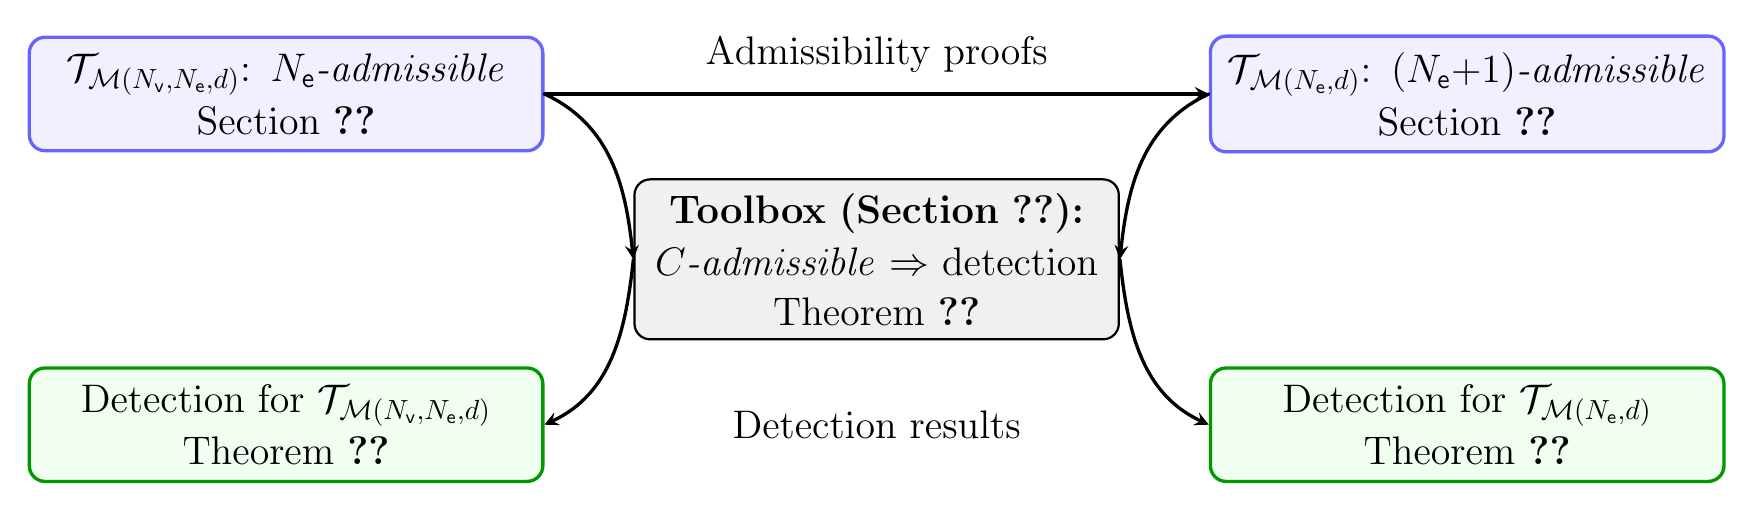
\begin{tikzpicture}[font=\Large, node distance=22mm and 32mm,
  >=stealth,
  nodeA/.style = {rectangle, rounded corners=2mm, draw=blue!60, fill=blue!6,
                  very thick, minimum height=12mm, text width=61mm,
                  align=center, inner sep=6pt},
  nodeD/.style = {rectangle, rounded corners=2mm, draw=green!60!black, fill=green!6,
                  very thick, minimum height=12mm, text width=61mm,
                  align=center, inner sep=6pt},
  toolbox/.style = {rectangle, rounded corners=2mm, draw=black, fill=black!6,
                    thick, minimum height=10mm, text width=58mm,
                    align=center, inner sep=5pt},
  flow/.style = {->, very thick, line cap=round},
  lab/.style  = {font=\scriptsize, text=black!65},
  ttl/.style  = {font=\Large}
]

\node[nodeA] (A1) at (-7.5,  2.1)
{$\mathcal{T}_{\mathcal{M}(N_{\mathsf v},N_{\mathsf e},d)}$: \emph{$N_{\mathsf{e}}$-admissible}\\[1pt] Section~\ref{subsec:bd-degree-specific}};

\node[nodeD] (A2) at (-7.5, -2.1)
{Detection for $\mathcal{T}_{\mathcal{M}(N_{\mathsf v},N_{\mathsf e},d)}$\\[1pt] Theorem~\ref{thm:bd-degree-motif-main}};

\node[nodeA] (D1) at ( 7.5,  2.1)
{$\mathcal{T}_{\mathcal{M}(N_{\mathsf e},d)}$: \emph{$(N_{\mathsf{e}}{+}1)$-admissible}\\[1pt] Section~\ref{subsec:general-bd-degree}};

\node[nodeD] (D2) at ( 7.5, -2.1)
{Detection for $\mathcal{T}_{\mathcal{M}(N_{\mathsf e},d)}$\\[1pt] Theorem~\ref{thm:bd-degree-motif-general}};

\node[ttl] at ($(A1)!0.5!(D1)+(0,5mm)$) {Admissibility proofs};
\node[ttl] at ($(A2)!0.5!(D2)$) {Detection results};

\coordinate (TopMid) at ($(A1)!0.5!(D1)$);
\coordinate (BotMid) at ($(A2)!0.5!(D2)$);
\node[toolbox] (TB) at ($(TopMid)!0.5!(BotMid)$)
{\textbf{Toolbox (Section~\ref{sec:general-motif}):}\\[1pt] \emph{$C$-admissible} $\Rightarrow$ detection\\ Theorem~\ref{thm:admissible}};

\draw[flow] (A1.east) to[out=-25,  in=96, looseness=1.00] (TB.west);
\draw[flow] (TB.west) to[out=264, in=25, looseness=1.00] (A2.east);

\draw[flow] (A1.east) to[out=0, in=180, looseness=1.05] (D1.west);

\draw[flow] (D1.west) to[out=205, in=84,  looseness=1.00] (TB.east);
\draw[flow] (TB.east) to[out=276, in=155, looseness=1.00] (D2.west);

\end{tikzpicture}%
}
\caption{Logical flow from admissibility to detection.}
\label{fig:logic-flow}
\end{figure}









\subsection{Construction of a Specific Bounded Degree Family}\label{subsec:bd-degree-specific}
%\nbr{Be consistent with capital letters in the titles}
For any integers $N_\sfv,N_\sfe$ such that $N_\sfv= \ell(d-1)+4$ and $N_\sfe = \binom{d}{2}\ell+d+1$ for some $\ell,d\in \mathbb N$, let $\maM(N_\sfv,N_\sfe,d)$ denote a special subset of bounded degree motifs with $N_\sfv$ vertices, $N_\sfe$ edges, and maximum degree $d$. Specifically, each motif $\sfM\in \maM(N_\sfv,N_\sfe,d)$ consists of $d-1$ paths of length $\ell$ between  two \emph{central vertices}, with each \emph{central vertex} connecting to an \emph{extremity vertex} of degree 1.
Additionally, there are $\ell$ red edges connecting distinct pairs of vertices between any two paths. The motif family $\maM(N_\sfv,N_\sfe,d)$ consists of all such motifs.
As illustrated in Figure~\ref{fig:bd-degree-graph}, each motif in $\maM(N_\sfv,N_\sfe,d)$ consists of 
$d-1$ paths, each in blue, with $\ell$ vertices of degree $d$. 
Specifically, each path is defined as $P_i\triangleq \sth{{v_{i,1}},v_{i,2},\cdots, v_{i,\ell}}$ for any $1\le i\le d-1$.
There are $\ell$ edges in red connecting distinct pairs of vertices between any two paths. 
Additionally, the \emph{central vertices} are $v_{01}, v_{02}$ and the \emph{extremity vertices} are $v_{00},v_{03}$.
%\nbr{comment or illustrate on special cases with small $d,\ell$?}
%The presence of two \emph{extremity vertices} with degree 1 makes the motifs in $\maM(N_\sfv,N_\sfe,d)$ highly irregular, and decreases the automorphism number for the motif in $\maM(N_\sfv,N_\sfe,d)$.

%Indeed, since there are only two vertices with degree 2 in $\sfM$, our construction can also be regarded as partially labeled graphs (see, e.g.~\citep[Section 3.2]{lovasz2012large}) with two labels on $v_{0,0}$ and $v_{0,3}$. When counting  such bounded degree motifs among $G_1$ and $G_2$, one can strat from such labeled vertices.
Indeed, since there are exactly two vertices of degree $2$ in $\sfM$, we may view $\sfM$ as a partially labeled graph with two distinguished vertices $v_{0,0}$ and $v_{0,3}$ (see, e.g., \citep[Section~3.2]{lovasz2012large}). When counting such bounded degree motifs in $G_1$ and $G_2$, one can start from these labeled vertices and extend along the prescribed paths.
Furthermore, this convention does not affect the statistic: if $\sfM$ admits an automorphism exchanging $v_{0,0}$ and $v_{0,3}$, the partially labeled count equals twice the unlabeled count; otherwise the two counts are identical.
This is equivalent to labeling the two \emph{central vertices} $v_{0,1}$ and $v_{0,2}$ while deleting the \emph{extremity vertices} $v_{0,0}$ and $v_{0,3}$. In the simple case $d=3$ and $\ell=1$, the motif then becomes a partially labeled square with one cross edge, illustrating the basic structure of this family.
%\nbr{Is is also equivalent to labeling $v_{0,1}$ and $v_{0,2}$ and deleting $v_{0,0}$ and $v_{0,3}$? Then $d=3,\ell=1$ is a partially labeled square with one cross edge.}


%\nbr{comments on labeled vertices, see \cite{lovasz2012large} (are they equivalent?)}

\begin{figure}
    \begin{center}
        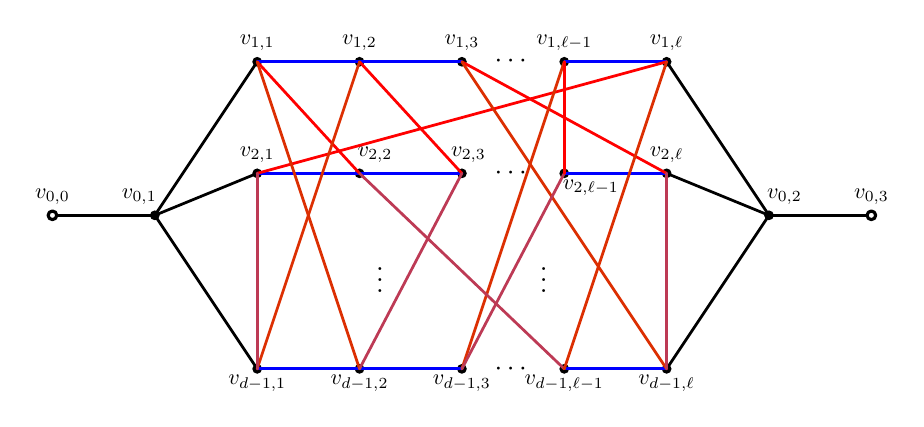
\begin{tikzpicture}[yscale = 1.3, xscale=1.3, line width=0.4mm, line cap=round, line join=round]

            % ---- node styles (match your refined motif figure) ----
            \tikzset{
              bullet/.style={circle, fill=black, inner sep=1.25pt},
              ep/.style={circle, draw=black, fill=white, inner sep=1.1pt}
            }

            % ---- endpoints: hollow circles ----
            \node[ep] (v00) at (-1,0) {};
            \node[ep] (v03) at (7,0) {};

            % ---- labels (keep your placements) ----
            \node[above,scale=0.8,yshift=1] at (v00) {$v_{0,0}$};
            \node[above,scale=0.8,xshift=-7,yshift=1] at (0,0) {$v_{0,1}$};
            \node[above,scale=0.8,yshift=1] at (1,1.5) {$v_{1,1}$};
            \node[above,scale=0.8,yshift=1] at (1,0.41) {$v_{2,1}$};
            \node[below,scale=0.8,yshift=1] at (1,-1.5) {$v_{d-1,1}$};
            \node[above,scale=0.8,yshift=1] at (2,1.5) {$v_{1,2}$};
            \node[above,scale=0.8,xshift=7,yshift=1] at (2,0.41) {$v_{2,2}$};
            \node[below,scale=0.8,yshift=1] at (2,-1.5) {$v_{d-1,2}$};
            \node[above,scale=0.8,yshift=1] at (3,1.5) {$v_{1,3}$};
            \node[above,scale=0.8,xshift=3,yshift=1] at (3,0.41) {$v_{2,3}$};
            \node[below,scale=0.8,yshift=1] at (3,-1.5) {$v_{d-1,3}$};
            \node[above,scale=0.8,yshift=1] at (4,1.5) {$v_{1,\ell-1}$};
            \node[below,scale=0.8,xshift=12,yshift=1] at (4,0.41) {$v_{2,\ell-1}$};
            \node[below,scale=0.8,yshift=1] at (4,-1.5) {$v_{d-1,\ell-1}$};
            \node[above,scale=0.8,yshift=1] at (5,1.5) {$v_{1,\ell}$};
            \node[above,scale=0.8,yshift=1] at (5,0.41) {$v_{2,\ell}$};
            \node[below,scale=0.8,yshift=1] at (5,-1.5) {$v_{d-1,\ell}$};
            \node[above,scale=0.8,yshift=1,xshift=7] at (6,0) {$v_{0,2}$};
            \node[above,scale=0.8,yshift=1] at (v03) {$v_{0,3}$};

            % ---- internal vertices: filled bullets ----
            \foreach \P in {
              (0,0),
              (1,1.5),(1,0.41),(1,-1.5),
              (2,1.5),(2,0.41),(2,-1.5),
              (3,1.5),(3,0.41),(3,-1.5),
              (4,1.5),(4,0.41),(4,-1.5),
              (5,1.5),(5,0.41),(5,-1.5),
              (6,0)
            }{
              \node[bullet] at \P {};
            }
            % NOTE: v00 and v03 already drawn as ep, so no bullet there.

            % ---- edges (unchanged) ----
            \draw[line width=0.35mm] (v00) -- (0,0);
            \draw[line width=0.35mm] (0,0) -- (1,1.5);
            \draw[line width=0.35mm] (0,0) -- (1,0.41);
            \draw[line width=0.35mm] (0,0) -- (1,-1.5);
            \draw[line width=0.35mm] (6,0) -- (v03);
            \draw[line width=0.35mm] (6,0) -- (5,1.5);
            \draw[line width=0.35mm] (6,0) -- (5,0.41);
            \draw[line width=0.35mm] (6,0) -- (5,-1.5);

            \draw[blue, line width=0.35mm] (1,1.5) -- (2,1.5);
            \draw[blue, line width=0.35mm] (2,1.5) -- (3,1.5);
            \draw[blue, line width=0.35mm] (1,0.41) -- (2,0.41);
            \draw[blue, line width=0.35mm] (2,0.41) -- (3,0.41);
            \draw[blue, line width=0.35mm] (1,-1.5) -- (2,-1.5);
            \draw[blue, line width=0.35mm] (2,-1.5) -- (3,-1.5);
            \draw[blue, line width=0.35mm] (4,1.5) -- (5,1.5);
            \draw[blue, line width=0.35mm] (4,0.41) -- (5,0.41);
            \draw[blue, line width=0.35mm] (4,-1.5) -- (5,-1.5);

            \draw (3.5,1.5) node{$\cdots$};
            \draw (3.5,0.41) node{$\cdots$};
            \draw (2.2,-0.55) node{$\vdots$};
            \draw (3.8,-0.55) node{$\vdots$};
            \draw (3.5,-1.5) node{$\cdots$};

            \draw[red1,line width=0.35mm] (1,1.5) -- (2,0.41);
            \draw[red1,line width=0.35mm] (2,1.5) -- (3,0.41);
            \draw[red1,line width=0.35mm] (3,1.5) -- (5,0.41);
            \draw[red1,line width=0.35mm] (5,1.5) -- (1,0.41);

            \draw[red2,line width=0.35mm] (2,1.5) -- (1,-1.5);
            \draw[red2,line width=0.35mm] (1,1.5) -- (2,-1.5);
            \draw[red2,line width=0.35mm] (3,1.5) -- (5,-1.5);
            \draw[red2,line width=0.35mm] (4,1.5) -- (3,-1.5);

            \draw[red3,line width=0.35mm] (1,0.41) -- (1,-1.5);
            \draw[red3,line width=0.35mm] (2,0.41) -- (4,-1.5);
            \draw[red3,line width=0.35mm] (4,0.41) -- (3,-1.5);
            \draw[red3,line width=0.35mm] (5,0.41) -- (5,-1.5);
            \draw[red3,line width=0.35mm] (3,0.41) -- (2,-1.5);

            \draw[red1,line width=0.35mm] (4,1.5) -- (4,0.41);
            \draw[red2,line width=0.35mm] (5,1.5) -- (4,-1.5);

        \end{tikzpicture}
    \end{center}
    \caption{A special bounded degree motif with vertex set size $N_\sfv$, edge set size $N_\sfe$, and maximum degree $d$.}
    \label{fig:bd-degree-graph}
\end{figure}

By Theorem~\ref{thm:admissible}, in order to provide a theoretical guarantee for $\maT_{\maM(N_\sfv,N_\sfe,d)}$, it suffices to verify the four \emph{$N_\sfe$-admissible} Conditions in Definition~\ref{def:admissible}. 
The connectivity for $\sfM\in \maM(N_\sfv,N_\sfe,d)$ yields the Condition~\ref{cond:connect}.
Since the vertices and edges for any $\sfM\in \maM(N_\sfv,N_\sfe,d)$ are bounded by $N_\sfe= \binom{d}{2}\ell+d+1$, Condition~\ref{cond:num} holds. We then verify Conditions~\ref{cond:signal-strength} and~\ref{cond:subgraph}, respectively. For Condition~\ref{cond:signal-strength}, since $\en(\sfM) = \en(\sfM')$ for any $\sfM,\sfM'\in \maM(N_\sfv,N_\sfe,d)$, the \emph{signal score} is characterized by $\sum_{\sfM\in \maM(N_\sfv,N_\sfe,d)}\rho^{2\en(\sfM)} = \rho^{2N_\sfe} |\maM(N_\sfv,N_\sfe,d)|$. The following lemma provides an estimate of $|\maM(N_\sfv,N_\sfe,d)|$.

\begin{lemma}\label{lem:motif-family-lwbd}
    For the motif family $ \maM(N_\sfv,N_\sfe,d)$  with $d\ge 3$, we have\begin{align}\label{eq:motif-family-lwbd}
        \frac{1}{2}\pth{\frac{2(N_\sfe-d-1)}{ed^{\frac{d}{d-2}}(d-1)}}^{\frac{d-2}{d}(N_\sfe-d-1)}\le |\maM(N_\sfv,N_\sfe,d)|\le \pth{\frac{2(N_\sfe-d-1)}{d(d-1)}}^{\frac{d-2}{d}(N_\sfe-d-1)}.
    \end{align}
\end{lemma}
 
The proof of Lemma~\ref{lem:motif-family-lwbd} is deferred to Appendix~\ref{apd:proof-lem-motif-family-lwbd}.
It follows from Lemma~\ref{lem:motif-family-lwbd} that, if $N_\sfe\ge d+1+ C(d) \rho^{-\frac{2d}{d-2}}$ with some constant $C(d)$, then \begin{align*}
    \sum_{\sfM\in \maM(N_\sfv,N_\sfe,d)}\rho^{2\en(\sfM)}&\ge \rho^{2N_\sfe}|\maM(N_\sfv,N_\sfe,d)|\\&\ge \frac{1}{2}\pth{\frac{2\rho^{\frac{2d}{d-2}}(N_\sfe-d-1)}{ed^{\frac{d}{d-2}}(d-1)}}^{\frac{d-2}{d}(N_\sfe-d-1)}\rho^{2d+2}\\&\ge\frac{1}{2}\pth{\frac{2C(d)}{ed^{\frac{d}{d-2}}(d-1)}}^{\frac{d-2}{d}C(d)\rho^{-2d/(d-2)}}\ge 400.
\end{align*} Hence, the requirement on the \emph{signal score} is satisfied. As for Condition~\ref{cond:subgraph}, we have the following Lemma.
\begin{lemma}\label{lem:subgraph}
    For any motif $\sfM\in \maM(N_\sfv,N_\sfe,d)$ and subgraph $\emptyset\neq \sfM'\subseteq \sfM$, we have %\nbr{need non-empty?}
    \begin{align*}
        d\,\vn(\sfM')\ge 2\,\en(\sfM')+1.
    \end{align*}
\end{lemma}

\begin{proof}
% [Proof of Lemma~\ref{lem:subgraph}]

We note that for any $v\in V(\sfM')$, the degree of $v$ is at most $d$. Therefore, we have $d \vn(\sfM')\ge 2 \en(\sfM')$. It remains to prove that the equality cannot be achieved.

    Suppose $d\vn(\sfM') = 2\en(\sfM')$. Then, for any $v\in V(\sfM')$, the degree of $v$ in $\sfM'$ is $d$. If there exists $1\le i\le d-1,1\le j\le \ell$ such that $v_{i,j}\in \sfM'$, since the degree of $v_{i,j}$ in $\sfM'$ is $d$, then $v_{i,{j+1}} \in \sfM'$. Similarly, we obtain that $v_{i,j},v_{i,j+1},\cdots, v_{i,\ell},v_{0,2},v_{0,3}\in V(\sfM')$. Since the degree of $v_{0,3}$ in $\sfM'$ is at most 1 and $d\ge 3$, we have $d\vn(\sfM')>2\en(\sfM')$. If there exists $0\le i\le 3$ such that $v_{0,i}\in V(\sfM')$, we can similarly obtain that $v_{0,0}\in V(\sfM')$ or $v_{0,3}\in V(\sfM')$, and thus $d\vn(\sfM')>2\en(\sfM')$. Therefore, we conclude that $d\vn(\sfM')\ge 2\en(\sfM')+1$ for any $\sfM\in \maM(N_\sfv,N_\sfe,d)$ and $\sfM'\subseteq \sfM$.
\end{proof}

Indeed, the presence of two \emph{extremity vertices} ensures that all motifs in \(\mathcal{M}(N_\sfv, N_\sfe, d)\) are non-regular.
For any connected motif $\mathsf{M}$ with maximum degree d, we have $2\en(\mathsf{M}')  \le d\vn(\mathsf{M}')$ for any subgraph $\mathsf{M}'\subseteq \mathsf{M}$.
The equality cannot hold, as the existence of two \emph{extremity vertices} of degree 1 prevents any subgraph from being $d$-regular.
Hence the inequality is strict, and hence the lemma follows.
By Lemma~\ref{lem:subgraph}, we have $n^{\vn(\sfM')}p^{\en(\sfM')}\ge n^{\frac{2\en(\sfM')+1}{d}}p^{\en(\sfM')}\ge n^{1/d}$ if $p\ge n^{-2/d}$. Taking $\epsilon_0 = \frac{1}{d}$ yields Condition~\ref{cond:subgraph}. Since $\sfM$ is connected and $N_\sfv\le N_\sfe$ by our construction, we obtain that the motif family $\maM(N_\sfv,N_\sfe,d)$ is \emph{$N_\sfe$-admissible}. Consequently, we obtain the following theorem regarding the detection performance of $\maT_{\maM(N_\sfv,N_\sfe,d)}$.
Let $[x]$ denote the greatest integer less than or equal to $x$.


\begin{theorem}\label{thm:bd-degree-motif-main}
     If $p=n^{-a}$ with $0<a\le \frac{2}{3}$ and  $d=\qth{\frac{2}{a}}$, when $N_\sfe=o\pth{\frac{\log n}{\max\pth{\log\log n,-\log\rho}}}$ and $N_\sfe\ge \frac{C_1(d)}{\rho^{2d/(d-2)}}$ for some constant $C_1(d)$ depending on $d$,\begin{align*}
        \maP_0\pth{\maT_{\maM(N_\sfv,N_\sfe,d)}\ge \tau}+\maP_1\pth{\maT_{\maM(N_\sfv,N_\sfe,d)}<\tau}\le 0.05.
    \end{align*}

    If $p=n^{-o(1)}$, then for any constant $\epsilon>0$, when $N_\sfe = o\pth{\frac{\log n}{\max\pth{\log\log n,-\log\rho}}}$ and $N_\sfe\ge \frac{C_2(\epsilon)}{\rho^{2+\epsilon}}$ for some constant $C_2(\epsilon)$ depending on $\epsilon$,\begin{align*}
        \maP_0\pth{\maT_{\maM(N_\sfv,N_\sfe,d)}\ge \tau}+\maP_1\pth{\maT_{\maM(N_\sfv,N_\sfe,d)}<\tau}\le 0.05.
    \end{align*}

    Furthermore, $\maT_{\maM(N_\sfv,N_\sfe,d)}$ is  computable in $O(n^{N_\sfe})$.
\end{theorem}

\begin{proof}
% [Proof of Theorem~\ref{thm:bd-degree-motif-main}]
We first show that $\maT_{\maM(N_\sfv,N_\sfe,d)}$ is computable in time $O(n^{N_\sfe})$. For any $\sfM\in \maM$, since there are $\binom{n}{\vn(\sfM)}(\vn(\sfM)!)$ injections from $V(\sfM)$ to $V(\bar{G}_1)$,
the injective homomorphism number $\inj(\sfM,\bar{G}_1)$ takes $\binom{n}{\vn(\sfM)}(\vn(\sfM)!)\le n^{\vn(\sfM)}$ time for computation. Similarly, the injective homomorphism number $\inj(\sfM,\bar{G}_2)$ can be computed in time $n^{\vn(\sfM)}$. Consequently, the time complexity for ${\maT_{\maM(N_\sfv,N_\sfe,d)}}$ is bounded by $2n^{\vn(\sfM)} |{\maM(N_\sfv,N_\sfe,d)}|$, and we have \begin{align*}
    2n^{\vn(\sfM)} |{\maM(N_\sfv,N_\sfe,d)}|&\overset{\mathrm{(a)}}{\le} 2n^{\ell(d-1)+4} \pth{\frac{2(N_\sfe-d-1)}{d(d-1)}}^{\frac{d-2}{d}\cdot (N_\sfe-d-1)}\\&\overset{\mathrm{(b)}}{\le} 2n^{2(N_\sfe+d-1)/d}(N_\sfe)^{N_\sfe}\overset{\mathrm{(c)}}{\le} n^{N_\sfe},
\end{align*}
where $\mathrm{(a)}$ is due to $\vn(\sfM)=\ell(d-1)+4$ and~\eqref{eq:motif-family-lwbd} in Lemma~\ref{lem:motif-family-lwbd}; $\mathrm{(b)}$ is because $\ell(d-1)+4 = \frac{2(N_\sfe+d-1)}{d}$, $\frac{2(N_\sfe-d-1)}{d(d-1)}\le N_\sfe$, and $\frac{d-2}{d}\cdot (N_\sfe-d-1)\le N_\sfe$; $\mathrm{(c)}$ is because $N_\sfe = o(\frac{\log n}{\log \log n})$ implies $2(N_\sfe)^{N_\sfe} = n^{o(1)}$ and $\frac{2(N_\sfe+d-1)}{d}\le \frac{2N_\sfe}{3}+2<N_\sfe$.

We then show the theoretical guarantee on $\maP_0\pth{\maT_{\maM(N_\sfv,N_\sfe,d)}\ge \tau}+\maP_1\pth{\maT_{\maM(N_\sfv,N_\sfe,d)}< \tau}$. By Theorem~\ref{thm:admissible}, it suffices to show that $\maM(N_\sfv,N_\sfe,d)$ is \emph{$C$-admissible}. Since $N_\sfv\le N_\sfe$ and $N_\sfe = o\pth{\frac{\log n}{\max \pth{\log \log n, -\log \rho}}}$, taking $C = N_\sfe$ yields Condition~\ref{cond:num}. By Lemma~\ref{lem:subgraph}, for all $\sfM\in \maM(N_\sfv,N_\sfe,d)$ and $\sfM'\subseteq \sfM$, we have \begin{align*}
    n^{\vn(\sfM')}p^{\en(\sfM')}\ge n^{(2\en(\sfM')+1)/d}p^{\en(\sfM')}\ge n^{1/d},
\end{align*}
where the last inequality is because $np^{d/2}\ge 1$ by the choice of $d$. Pick $\epsilon_0 = 1/d$, we conclude the Condition~\ref{cond:subgraph} in Definition~\ref{def:admissible}. Since all $\sfM\in \maM(N_\sfv,N_\sfe,d)$ are connected, it remains to verify the Condition~\ref{cond:signal-strength} $\sum_{\sfM\in \maM}\rho^{2\en(\sfM)}\ge 400$.

We first focus on the case $p = n^{-a}$ with $0<a\le \frac{2}{3}$. By Lemma~\ref{lem:motif-family-lwbd}, \begin{align*}
    \sum_{\sfM\in \maM(N_\sfv,N_\sfe,d)}\rho^{2\en(\sfM)}\ge \frac{1}{2}\pth{\frac{2(N_\sfe-d-1)}{ed^{\frac{d}{d-2}}(d-1)}}^{\frac{d-2}{d}(N_\sfe-d-1)}\rho^{2d+2}.
\end{align*}
We first prove that there exists a constant $C(d)$ depending on $d$ such that \begin{align*}
    \frac{1}{2}(C(d))^{\frac{d-2}{d}\rho^{-2d/(d-2)}}\rho^{2d+2}\ge 400
\end{align*}
for any $0\le \rho\le 1$ and integer $d\ge 3$.
Pick $C(d) = \exp\pth{3\log 800+\frac{d(2d+2)}{d-2}}$. Then, \begin{align*}
    &~\frac{d-2}{d}\rho^{-\frac{2d}{d-2}}\log (C(d))+(2d+2)\log\rho \\=&~ \frac{d-2}{d}\rho^{-\frac{2d}{d-2}}\pth{3\log 800+\frac{d(2d+2)}{d-2}}+(2d+2)\log\rho\\\overset{\mathrm{(a)}}{\ge}&~ \frac{3(d-2)\log(800)}{d}+(2d+2)\pth{\frac{1}{\rho^2}+\log \rho}\overset{\mathrm{(b)}}{\ge}   \log 800,
\end{align*}
where $\mathrm{(a)}$ is because $\rho\le 1$ and $\frac{2d}{d-2}\ge 2$; $\mathrm{(b)}$ follows from $\log x+\frac{1}{x^2}\ge 0$ for any $x>0$ and $\frac{3(d-2)}{d}\ge 1$ for any $d\ge 3$. Therefore, we obtain $\frac{1}{2}(C(d))^{\frac{d-2}{d}\rho^{-2d/(d-2)}} \rho^{2d+2}\ge 400$. Let $C_1(d)\triangleq d+1+\frac{1}{2}e d^{d/(d-2)} (d-1) C(d)$. When $N_\sfe\ge \frac{C_1(d)}{\rho^{2d/(d-2)}}$, we have \begin{align*}
    \frac{2(N_\sfe-d-1)\rho^{2d/(d-2)}}{ed^{d/(d-2)}(d-1)} &\ge \frac{2C_1(d) - 2(d+1) \rho^{2d/(d-2)}}{ed^{d/(d-2)}(d-1)} \ge \frac{2C_1(d) - 2(d+1)}{ed^{d/(d-2)}(d-1)} = C(d)
\end{align*}
and \begin{align*}
    \frac{d-2}{d}\cdot (N_\sfe-d-1) \ge \frac{d-2}{d}\cdot\pth{\frac{d+1}{\rho^{2d/(d-2)}}-d-1} \ge \frac{d-2}{d} \rho^{-\frac{2d}{d-2}}.
\end{align*}
Therefore, \begin{align*}
    \sum_{\sfM\in \maM(N_\sfv,N_\sfe,d)}\rho^{2\en(\sfM)} &\ge \frac{1}{2} \pth{\frac{2(N_\sfe-d-1)\rho^{2d/(d-2)}}{ed^{d/(d-2)}(d-1)}}^{\frac{d-2}{d}\cdot (N_\sfe-d-1)}\rho^{2d+2}\\&\ge \frac{1}{2}(C(d))^{\frac{d-2}{d}\rho^{-2d/(d-2)}} \rho^{2d+2}\ge 400.
\end{align*} 

We then focus on the case $p = n^{o(1)}$. For any $\epsilon>0$, pick $d = \qth{\frac{4}{\epsilon}}+3$. Then $\frac{2d}{d-2}<2+\epsilon$. Let $C_2(\epsilon)\triangleq C_1\pth{\qth{\frac{4}{\epsilon}}+3}$. We have shown that when $N_\sfe\ge \frac{C_1(d)}{\rho^{2d/(d-2)}}$, we have $\sum_{\sfM\in \maM(N_\sfv,N_\sfe,d)}\rho^{2\en(\sfM)}\ge 400$.
Since $\frac{C_1(d)}{\rho^{2d/(d-2)}} \le \frac{C_2(\epsilon)}{\rho^{2+\epsilon}}$, we also have $\sum_{\sfM\in \maM(N_\sfv,N_\sfe,d)}\rho^{2\en(\sfM)}\ge 400$.
Consequently, $\maM(N_\sfv,N_\sfe,d)$ is \emph{$N_\sfe$-admissible}. By Theorem~\ref{thm:admissible}, we obtain that \begin{equation*}
\maP_0\pth{\maT_{\maM(N_\sfv,N_\sfe,d)}\ge \tau}+\maP_1\pth{\maT_{\maM(N_\sfv,N_\sfe,d)}< \tau}\le 0.05.\qedhere
\end{equation*}
\end{proof}

%The proof of Theorem~\ref{thm:bd-degree-motif-main} is deferred to Appendix~\ref{apd:proof-thm-speci}.
By Lemmas~\ref{lem:motif-family-lwbd} and~\ref{lem:subgraph}, the bounded degree motif family $\maM(N_\sfv,N_\sfe,d)$ is \emph{$N_\sfe$-admissible}.
In view of Theorem~\ref{thm:bd-degree-motif-main}, if $\rho$ is a constant, one can choose a constant $N_\sfe$ when $p \ge n^{-2/3}$, making the test statistic computable in polynomial time. Although the test statistic $\maT_{\maM(N_\sfv,N_\sfe,d)}$ suffices for correlation detection, the motifs in $\maM(N_\sfv,N_\sfe,d)$ are highly specialized and uncommon in practical scenarios; for instance, triangles and quadrilaterals are not included in this family. To obtain a more broadly applicable motif-counting statistic, we will show in Section~\ref{subsec:general-bd-degree} that counting all bounded degree motifs also suffices for correlation detection. 
%Consequently, the polynomial-time test statistic $\maT_{\maM(N_\sfv,N_\sfe,d)}$ succeeds for detection for any constant correlation $\rho$ when $p\ge n^{-2/3}$.


\subsection{A General Admissible Statistic}\label{subsec:general-bd-degree}
In this subsection, we consider an implementable test statistic $\maT_{\maM(N_\sfe,d)}$, where $\maM(N_\sfe,d)$ denotes the set of all connected motifs with $N_\sfe$ edges and maximum degree at most $d$. In order to provide theoretical guarantee, we show that $\maT_{\maM(N_\sfe,d)}$ is  \emph{$(N_\sfe{+}1)$-admissible}. We then verify the conditions in Definition~\ref{def:admissible}:\begin{enumerate}
    \item Since all $\sfM\in \maM(N_\sfe,d)$ are connected, we have  $\vn(\sfM)\le \en(\sfM)+1\le N_\sfe+1$, where the equality holds when $\sfM$ is a tree;
    \item Since $\maM(N_\sfv,N_\sfe,d)\subseteq \maM(N_\sfe,d)$, we have $$\sum_{\sfM\in \maM(N_\sfe,d)} \rho^{2\en(\sfM)}\ge \sum_{\sfM\in \maM(N_\sfv,N_\sfe,d)} \rho^{2\en(\sfM)}\ge 400;$$
    \item For all $\sfM\in\maM(N_\sfe,d)$ and subgraph $\sfM'\subseteq \sfM$, since the maximum degree of $\sfM'$ is bounded by $d$, we have $\en(\sfM')\le \frac{d}{2}\vn(\sfM')$. Consequently, when $p\ge n^{-a}$ for some constant $a<\frac{2}{3}$, one can pick $d\ge 3$  such that $1-\frac{da}{2}>0$, yielding $n^{\vn(\sfM')} p^{\en(\sfM')}\ge (np^{d/2})^{\vn(\sfM')}\ge n^{1-\frac{da}{2}}$.
    \item For all $\sfM\in \maM(N_\sfe,d)$, $\sfM$ is connected.
\end{enumerate}


%Indeed, for any $\sfM'\subseteq \sfM$ and $\sfM\in \maM(N_\sfe,d)$, since the maximum degree of $\sfM'$ is bounded by $d$, we have $\en(\sfM')\le \frac{d}{2}\vn(\sfM')$. Consequently, when $p\ge n^{-a}$ for some constant $a<\frac{2}{3}$, one can pick $d\ge 3$  such that $1-\frac{da}{2}>0$, yielding $n^{\vn(\sfM')} p^{\en(\sfM')}\ge (np^{d/2})^{\vn(\sfM')}\ge n^{1-\frac{da}{2}}$. For the \emph{signal score}, note that $\maM(N_\sfv,N_\sfe,d)\subseteq \maM(N_\sfe,d)$, which implies
%\begin{align*}
%    \sum_{\sfM\in \maM(N_\sfe,d)} \rho^{2\en(\sfM)}\ge \sum_{\sfM\in \maM(N_\sfv,N_\sfe,d)} \rho^{2\en(\sfM)}.
%\end{align*}
Therefore, the bounded degree motif counting statistic $\maT_{\maM(N_\sfe,d)}$ is \emph{$(N_\sfe{+}1)$-admissible} whenever $\maT_{\maM(N_\sfv,N_\sfe,d)}$ is \emph{$N_\sfe$-admissible} and $p\ge n^{-a}$ for some constant $a<\frac{2}{3}$. Specifically, we have the following Theorem.
\begin{theorem}\label{thm:bd-degree-motif-general}
      If $p=n^{-a}$ with constant $0<a< \frac{2}{3}$, then for $d=3\cdot \indc{\frac{2}{5}<a<\frac{2}{3}}+\pth{\qth{\frac{2}{a}}-1}\cdot \indc{0<a\le \frac{2}{5}}$, when $N_\sfe=o\pth{\frac{\log n}{\max\pth{\log\log n,-\log\rho}}}$ and $N_\sfe\ge \frac{C_1(d)}{\rho^{2d/(d-2)}}$ for some constant $C_1(d)$ depending on $d$,\begin{align*}
        \maP_0\pth{\maT_{\maM(N_\sfe,d)}\ge \tau}+\maP_1\pth{\maT_{\maM(N_\sfe,d)}<\tau}\le 0.05.
    \end{align*}

    If $p=n^{-o(1)}$, then for any constant $\epsilon>0$, when $N_\sfe = o\pth{\frac{\log n}{\max\pth{\log\log n,-\log\rho}}}$ and $N_\sfe\ge \frac{C_2(\epsilon)}{\rho^{2+\epsilon}}$ for some constant $C_2(\epsilon)$ depending on $\epsilon$,\begin{align*}
        \maP_0\pth{\maT_{\maM(N_\sfe,d)}\ge \tau}+\maP_1\pth{\maT_{\maM(N_\sfe,d)}<\tau}\le 0.05.
    \end{align*}

    Furthermore, $\maT_{\maM(N_\sfe,d)}$ is  computable in time $O(n^{N_\sfe+1+o(1)})$.
\end{theorem}
\begin{proof}
% [Proof of Theorem~\ref{thm:bd-degree-motif-general}]

We first show that the statistic $\maT_{\maM(N_\sfv,N_\sfe,d)}$ is computable in time $O(n^{N_\sfe+1+o(1)})$. Recall that the injective homomorphism number $\inj(\sfM,\bar{G}_1),\inj(\sfM,\bar{G}_2)$ can be computed in time $2n^{\vn(\sfM)}$. Since for connected  motif $\sfM$ with $N_\sfe$ edges, the number of vertices is bounded by $N_\sfe+1$, the total computation time is then bounded by $2n^{N_\sfe+1}|\maM(N_\sfe,d)|$. We then upper bound $|\maM(N_\sfe,d)|$. We note that \begin{align*}
    |\maM(N_\sfe,d)|
\le \sum_{N_\sfv=1}^{N_\sfe+1}\binom{\binom{N_\sfv}{2}}{N_\sfe}
\le (N_\sfe+1)\binom{\binom{N_\sfe+1}{2}}{N_\sfe}
\le (N_\sfe+1)\pth{\frac{e(N_\sfe+1)}{2}}^{N_\sfe},
\end{align*}
where the first inequality is because $1\le N_\sfv\le N_\sfe+1$ and there are at most $\binom{N_\sfv}{2}$ edges with $N_\sfv$ vertices; the last inequality is because $\binom{m_1}{m_2}\le\pth{\frac{em_1}{m_2}}^{m_2}$ for all $m_1,m_2\in \mathbb{N}$. Since $N_e = o\pth{\frac{\log n}{\log \log n}}$, we have $(N_\sfe+1)\pth{\frac{e(N_\sfe+1)}{2}}^{N_\sfe} = n^{o(1)}$. Consequently, the overall computation time is $n^{N_\sfe+1+o(1)}$.


We then show the theoretical guarantee. We prove that $\maM(N_\sfe,d)$ is \emph{$(N_\sfe{+}1)$-admissible}.
For Condition~\ref{cond:num}, since there are at most $N_\sfe+1$ vertices in a connected motif with $N_\sfe$ edges, choosing $C = N_\sfe +1$ satisfies the Condition~\ref{cond:num}. Since $\maM(N_\sfv,N_\sfe,d)\subseteq \maM(N_\sfe,d)$ and $\maM(N_\sfv,N_\sfe,d)$ is \emph{$N_\sfe$-admissible}, we have \begin{align*}
    \sum_{\sfM\in \maM(N_\sfe,d)}\rho^{2\en(\sfM)}\ge  \sum_{\sfM\in \maM(N_\sfv, N_\sfe,d)}\rho^{2\en(\sfM)}\ge 400.
\end{align*}
For Condition~\ref{cond:subgraph}, since the maximum degree of all $\sfM\in\maM$ is bounded by $d$, we have $\en(\sfM')\le \frac{d}{2}\vn(\sfM')$ for all $\sfM'\subseteq \sfM$. When $p=n^{o(1)}$, we have $n^{\vn(\sfM')}p^{\en(\sfM')}\ge n^{1/2}$.
When $p = n^{-a}$ with constant $0<a\le \frac{2}{5}$, we pick $d = \qth{\frac{2}{a}}-1$. Since $d\le \frac{2}{a}-1$,  we have \begin{align*}
    n^{\vn(\sfM')}p^{\en(\sfM')}&\ge n^{\vn(\sfM')}p^{d\vn(\sfM')/2}\ge (np^{(2/a-1)/2})^{\vn(\sfM')}\\&=(n^{a/2})^{\vn(\sfM')}\ge n^{a/2}.
\end{align*}
When $p=n^{-a}$ with constant $\frac{2}{5}<a<\frac{2}{3}$, we pick $d=3$.
Consequently, 
\begin{align*}
    n^{\vn(\sfM')}p^{\en(\sfM')}&\ge n^{\vn(\sfM')}p^{d\vn(\sfM')/2}\\&=(n^{1-3a/2})^{\vn(\sfM')}\ge n^{1-3a/2}.
\end{align*}
Picking $\epsilon_0 = \min\pth{\frac{a}{2},1-\frac{3a}{2}}$ yields the Condition~\ref{cond:subgraph} in Definition~\ref{def:admissible}. Since all $\sfM\in \maM(N_\sfe,d)$ are connected, we conclude that $\maM(N_\sfe,d)$ is \emph{$C$-admissible}. By Theorem~\ref{thm:admissible}, we have \begin{equation*}
    \maP_0(\maT_{\maM(N_\sfe,d)}\ge\tau)+\maP_1(\maT_{\maM(N_\sfe,d)}<\tau)\le 0.05.\qedhere
\end{equation*}
\end{proof}
%The proof of Theorem~\ref{thm:bd-degree-motif-general} is deferred to Appendix~\ref{apd:proof-thm-general}.
In view of Theorem~\ref{thm:bd-degree-motif-general}, we have shown that the bounded degree motif counting statistic $\maT_{\maM(N_\sfe,d)}$ is sufficient for detection when $p \ge n^{-a}$ for some constant $0 < a < \frac{2}{3}$. 
The parameter $d$ is selected to ensure the Condition~\ref{cond:subgraph} in Definition~\ref{def:admissible}.
Moreover, for constant correlation $\rho$, one can choose a constant $N_\sfe$ satisfying the required conditions, making the test statistic computable in polynomial time $O(n^{N_\sfe+1+o(1)})$. %\nbr{check polynomial order}.
Compared with the statistic $\maT_{\maM(N_\sfv,N_\sfe,d)}$ in Theorem~\ref{thm:bd-degree-motif-main}, the theoretical guarantee for $\maT_{\maM(N_\sfe,d)}$ requires a slightly stronger condition on the edge probability, namely $p \ge n^{-a}$ with $0<a<\frac{2}{3}$. Nevertheless, $\maT_{\maM(N_\sfe,d)}$ is better aligned with applications, as the bounded degree motif family $\maM(N_\sfe,d)$ includes many commonly occurring motifs. 
Although the condition $p \ge n^{-2/3}$ plays an important role in the analysis of the motif-counting statistics $\maT_{\maM(N_\sfv, N_\sfe,d)}$ and $\maT_{\maM(N_\sfe,d)}$, it is not a necessary requirement for admissible motif families. In fact, for sparser graphs with $p < n^{-2/3}$, \cite{mao2024testing} showed that tree counting remains successful for detection under an additional constraint $\rho^2 \ge \alpha \approx 0.338$; moreover, the corresponding tree-counting statistic is also admissible. More generally, in such sparser regimes, detection remains feasible as long as the admissibility is satisfied.

Indeed, one could consider a larger motif family than $\maM(N_\sfe,d)$, such as the family containing all bounded degree motifs with at most $N_\sfe$ edges rather than exactly $N_\sfe$. While this would increase the signal and the theoretical guarantee could be established similarly, such a choice may introduce practical challenges.
Recall that we select the weight $\omega_\sfM = \frac{\rho^{\en(\sfM)} (n-\vn(\sfM))!}{n!\,(p(1-p))^{\en(\sfM)}\aut(\sfM)}.$
Since the correlation parameter $\rho$ is challenging to estimate in practice, it is natural to restrict attention to motifs with the same number of edges. Notably, the family $\maM(N_\sfe,d)$ satisfies this property and remains practical. We will demonstrate in Section~\ref{sec:num-results} that the statistic $\maT_{\maM(N_\sfe,d)}$ performs well on synthetic data.



%\subsection{Interpretations of the results}

 
%We then present the theoretical guarantee in the \ER model. By selecting bounded degree motif counting estimator, we give an upper bound on the sum of Type I and Type II errors. Specifically, we show that $\E_{\maP_1}\qth{\maT} - \E_{\maP_0}\qth{\maT} \ge C\max\sth{\sqrt{\var_\maP(\maT)},\sqrt{\var_{\maP_0}(\maT)}}$ for some sufficiently large constant $C$. By setting the threshold as $\tau = \frac{1}{2}\pth{\E_{\maP_0}(\maT)+\E_{\maP_1}(\maT)}$, we can control the sum of Type I and Type II errors using Chebyshev's inequality.


%\begin{theorem}\label{thm:main}
%If $p=n^{-a }$ with $0<a\le \frac{2}{3}$, then for any constant $c>0$ and $d=\qth{\frac{2}{\alpha}}$, when $\en(\maM) = o(\frac{\log n}{\max\sth{\log \log n,-\log \rho}})$ and $\en(\maM)\ge \frac{C_1\pth{c,d}}{\rho^{ {2d/(d-2)}}}$, there exists an estimator $\maT$ computable in time $n^{\en(\maM)}$ and a threshold $\tau$ such that,
%\begin{align*}
%    \maP\pth{\maT< \tau}+{\maP_0}\pth{\maT\ge \tau}\le c,
%\end{align*}
%where $C_1(c,d)$ is a constant depending on $c$ and $d$.

%If $p=n^{-o(1)}$,
%then for any constants $c,\epsilon>0$, when  $\en(\maM) = o(\frac{\log n}{\max\sth{\log \log n,-\log \rho}})$ and $\en(\maM) \ge \frac{C_2(c,\epsilon)}{\rho^{2+\epsilon}}$, there exists an estimator $\maT$ computable in  time  $n^{\en(\maM)}$ and a threshold $\tau$ such that,
%\begin{align*}
%    \maP\pth{\maT< \tau}+{\maP_0}\pth{\maT\ge \tau}\le c,
%\end{align*}
%where $C_2(c,\epsilon)$ is a constant depending on $c$ and $\epsilon$.
%\end{theorem}

Theorems~\ref{thm:bd-degree-motif-main} and~\ref{thm:bd-degree-motif-general} provide sufficient conditions for detection, leading to a  degree-$O(\rho^{-2d/(d-2)})$ algorithm  when $p = n^{-a}$ for any $0<a\le \tfrac{2}{3}$. When $p=n^{-o(1)}$, there exists a degree-$O(\rho^{-2-\epsilon})$ algorithm for any $\epsilon>0$.
When the maximum degree satisfies $d \le 2$, the  connected motifs reduce to paths and cycles, which provide limited structural information for detection. Hence, we consider bounded degree motifs with $d \ge 3$; this choice underlies the coefficient $\tfrac{2}{3}$ appearing in the detection threshold.
Indeed, the size of the motif family $\maM$ plays a crucial role in controlling errors. Specifically, in order to achieve detection for any constant $\rho$, it is necessary that $|\maM|\asymp \en(\maM)^{\en(\maM)}$. As a result, it is natural to consider the motifs with maximum degree $d\ge 3$. 
The condition  $\en(\maM) = o(\frac{\log n}{\max\sth{\log \log n,-\log \rho}})$, $\en(\maM)\ge \frac{C_1\pth{d}}{\rho^{ {2d/(d-2)}}}$, and $\en(\maM)\ge \frac{C_2(\epsilon)}{\rho^{2+\epsilon}}$ implies a necessary constraint on the correlation coefficient, namely, $\rho \gtrsim \frac{1}{\log n}$. In fact, counting motifs with $\en(\maM)$ edges in $\bar{G}_1$ and $\bar{G}_2$ corresponds to a degree-$\en(\maM)$ polynomial algorithm.
In particular, when $\rho$ is a constant, the time complexity remains polynomial. 
For  $p\ge n^{-1/3}$ and any constant $\rho$, \cite{barak2019nearly}
achieved detection criteria by counting balanced graphs, whereas~\cite{mao2024testing} succeeded when $p\ge n^{-1+o(1)}$ and $\rho \ge \sqrt{\alpha}$ by counting trees.
Our bounded degree counting method bridges the gap between these regimes by establishing detection for $p\in [n^{-2/3},n^{-1/3}]$ with constant $\rho <\sqrt{\alpha}$.
Beyond motif counting approaches, \cite{ding2023polynomial} proposed an iterative method that can be applied to both detection and the recovery of $\pi$ under $\maH_1$, achieving reliable performance for any constant $\rho$ when $p \ge n^{-1+\delta}$ with a small constant $\delta$. We will show in Section~\ref{sec:refined-results} that detection remains achievable in this regime via a more refined construction.

%\nbr{How about the iterative algorithm \cite{ding2023polynomial}?}
%\nbr{add refs on previous algorithms with $n^{-1/3}$?} 
%See Figure~\ref{fig:phase-diagram} for further details.

Indeed, our results align with computational hardness conjectures in this problem.
It has been postulated in~\cite{hopkins2017efficient,hopkins2018statistical} that the framework of low-degree polynomial algorithms  captures the hardness of detecting and recovering latent structures. Based on the low-degree conjecture, \cite{ding2023low} showed that any degree-$O(\rho^{-1})$ polynomial algorithm fails for detection with vanishing error when $p = n^{-\alpha}$ for any constant $\alpha\in (0,1)$. The more recent work~\cite{li2025algorithmic} provided evidence on the detection problem and conjectured that any degree-$o(\rho^{-1})$ polynomial algorithm fails for detection with constant error. In summary, our bounded degree motif counting statistic provides a polynomial-time algorithm that aligns with the low-degree conjecture, achieving a gap of $\frac{2d}{d-2}$ in the sparse regime and a gap of $2+\epsilon$ in the dense regime in terms of the exponent of $1/\rho$.







\begin{remark}[Trade-off between computation and statistical efficiency]
As shown in Theorems~\ref{thm:bd-degree-motif-main} and~\ref{thm:bd-degree-motif-general}, there exist conditions on $N_\sfe$ to satisfy the detection criterion $0.05$. %Specifically, the constants $C_1(d)$ and $C_2(\epsilon)$ both decrease as $c$ decreases. 
To achieve stronger statistical efficiency, it is necessary to count motifs with a larger number of edges. However, if the detection criterion satisfies $$\limsup_{n\to\infty}\qth{\maP_0(\maT\ge \tau)+\maP_1(\maT<\tau)} = o(1),$$ then $N_\sfe = \omega(1)$ as $n \to \infty$, and the corresponding test statistic is no longer computable in polynomial time. Consequently, there exists a trade-off between computation time and statistical efficiency.
\end{remark}

%\begin{remark}[Generalization to other graph models]
%    Apart from the correlated \ER model, another important model is the Gaussian Wigner model, where the correlated edges follow a standard normal distribution with correlation $\rho$ and the independent edges follow independent standard normal distributions. In this setting, the bounded degree motif counting estimator $\maT_{\maM(N_\sfe,d)}$ suffices for detection in Gaussian Wigner model when the correlation $\rho$ is a constant, and it is also a polynomial-time algorithm. The main proof for controlling the Type I and Type II errors follows a similar structure.
%\end{remark}



\section{Extension to the Sparser Regime via Refined Motif Classes}\label{sec:refined-results}

In Section~\ref{sec:bd-sub-count}, we show that counting a bounded degree motif family suffices for correlation detection for any constant $\rho=\Omega(1)$ when $p\ge n^{-2/3}$; see Theorem~\ref{thm:bd-degree-motif-main}. This exponent $2/3$ is not intrinsic. Indeed, it stems from the technical Condition~\ref{cond:subgraph} in Definition~\ref{def:admissible}, which requires $n^{\vn(\sfM')}p^{\en(\sfM')}\ge n^{\epsilon_0}$ for all $\sfM\in\maM$ and all nonempty subgraphs $\emptyset\neq \sfM'\subseteq \sfM$. When choosing $\maM(N_\sfv,N_\sfe,d)$ (or $\maM(N_\sfe,d)$), we can only control the density ratio $\en(\sfM')/\vn(\sfM')$ by a constant close to $3/2$. Consequently, enforcing Condition~\ref{cond:subgraph} yields the constraint $p\ge n^{-2/3}$. On the other hand, it follows from~\cite{ding2023low} that when $p=n^{-1+o(1)}$, there is evidence from the low-degree perspective that the correlation constraint $\rho^2\ge \alpha\approx 0.338$ is tight. It is then natural to ask:
\begin{center}
\emph{Can we design a finer motif family so that motif counting succeeds when $p\ge n^{-1+\delta}$?}
\end{center}


To extend the regime $p\ge n^{-2/3}$ to the sparser regime $p\ge n^{-1+\delta}$ for any given constant $\delta>0$, we need to construct a motif family $\maM$ such that, for every $\sfM\in\maM$ and every nonempty subgraph $\emptyset\neq \sfM'\subseteq \sfM$, the edge--vertex density satisfies $\en(\sfM')/\vn(\sfM')\le 1/(1-\delta)$, while keeping the family size at most $(c_1 N_\sfe)^{c_2 N_\sfe}$. Recall the construction in Figure~\ref{fig:bd-degree-graph} for $d=3$. There, most vertices have degree $3$, which leads to a relatively large edge--vertex density. In what follows, we construct a new motif family in which degree-$3$ vertices are rare. In fact, their proportion is controlled by $\delta$ and all remaining vertices have degree $1$ or $2$.

We then introduce the construction for $\overline{\maM}(N_\sfv,N_\sfe,3)$ such that $N_\sfv = t(6\ell -1)-2\ell+3$ and $N_\sfe= t(6\ell-1)+2$, where $t,\ell\ge 1$ are integers.
See Figure~\ref{fig:refined-motif}.
For simplicity, we denote the dashed edge by a path of $t+1$ vertices connecting two vertices. For instance, there are $t-1$ vertices between $v_{1,1}$ and $v_{1,2}$. For each $\overline{\maM}(N_\sfv,N_\sfe,3)$, the construction consists of the following three steps:\begin{enumerate}
    \item Construct $\ell$ cycles of length $4t$ (in red color), with $4\ell$ special vertex $v_{i,1},v_{i,2},v_{i,3},v_{i,4}$ for $1\le i\le \ell$ and remaining normal vertices. The special vertices will be of degree 3 and the remaining vertices will be of degree 2. There are $t-1$ vertices between $(v_{i,1},v_{i,2}),(v_{i,2},v_{i,3}),(v_{i,3},v_{i,4}),(v_{i,4},v_{i,1})$, respectively. 
    \item Connect $v_{i,3}$ and $v_{i+1,1}$ with a dashed edge (i.e., there are $t-1$ vertices between them) and connect $(v_{0,0},v_{1,1}),(v_{\ell,3},v_{0,1})$, where $v_{0,0},v_{0,1}$ are two extremity vertices.
    \item\label{item:refined-step3} Arbitrarily select a permutation $\sigma:[\ell]\mapsto [\ell]$. Connect $v_{i,2}$ to $v_{\sigma(i),4}$ with a dashed edge (in blue color) for all $1\le i\le \ell$.
\end{enumerate}




\begin{figure}[htbp]
  \begin{center}
    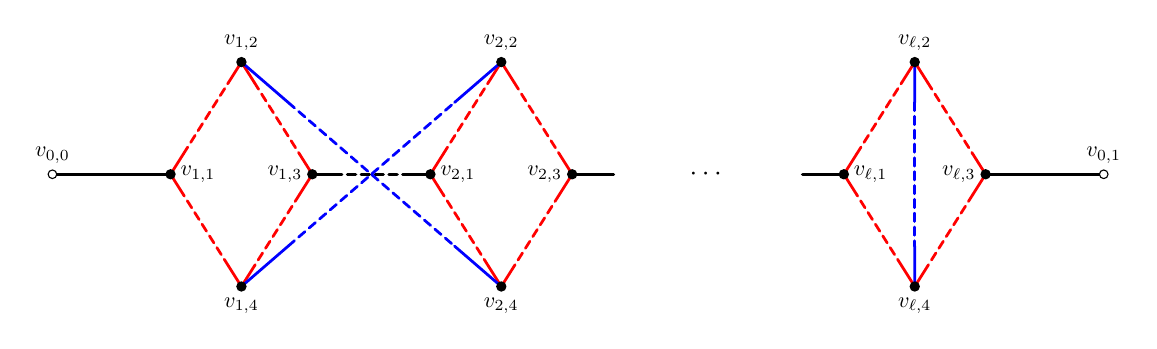
\begin{tikzpicture}[yscale=1.5, xscale=1.5, line cap=round, line join=round]

      % ---- stub--dashed helpers (local) ----
      \def\stubfrac{0.18}
      \newcommand{\stubdashed}[2]{%
        \draw[line width=0.4mm]
          (#1) -- ($(#1)!\stubfrac!(#2)$);
        \draw[densely dashed, line width=0.4mm]
          ($(#1)!\stubfrac!(#2)$) -- ($(#2)!\stubfrac!(#1)$);
        \draw[line width=0.4mm]
          ($(#2)!\stubfrac!(#1)$) -- (#2);
      }
      \newcommand{\redstubdashed}[2]{%
        \draw[red, line width=0.35mm]
          (#1) -- ($(#1)!\stubfrac!(#2)$);
        \draw[red, densely dashed, line width=0.35mm]
          ($(#1)!\stubfrac!(#2)$) -- ($(#2)!\stubfrac!(#1)$);
        \draw[red, line width=0.35mm]
          ($(#2)!\stubfrac!(#1)$) -- (#2);
      }
      \newcommand{\bluestubdashed}[2]{%
        \draw[blue, line width=0.35mm]
          (#1) -- ($(#1)!\stubfrac!(#2)$);
        \draw[blue, densely dashed, line width=0.35mm]
          ($(#1)!\stubfrac!(#2)$) -- ($(#2)!\stubfrac!(#1)$);
        \draw[blue, line width=0.35mm]
          ($(#2)!\stubfrac!(#1)$) -- (#2);
      }

      % =========================
      % Coordinates (compact)
      % =========================
      \coordinate (L) at (0,0);
      \coordinate (R) at (8.9,0); % equal tail length: 1.0 on both sides

      % Diamond 1
      \coordinate (D1l) at (1.0,0);
      \coordinate (D1t) at (1.6,0.95);
      \coordinate (D1r) at (2.2,0);
      \coordinate (D1b) at (1.6,-0.95);

      % Diamond 2
      \coordinate (D2l) at (3.2,0);
      \coordinate (D2t) at (3.8,0.95);
      \coordinate (D2r) at (4.4,0);
      \coordinate (D2b) at (3.8,-0.95);

      % Diamond 3 (last)
      \coordinate (D3l) at (6.7,0);
      \coordinate (D3t) at (7.3,0.95);
      \coordinate (D3r) at (7.9,0);
      \coordinate (D3b) at (7.3,-0.95);

      % =========================
      % Labels (placed in blank space)
      % Endpoints: v_{0,0}, v_{0,1}
      % Each diamond (left, top, right, bottom):
      %   Diamond 1: v_{1,1}, v_{1,2}, v_{1,3}, v_{1,4}
      %   Diamond 2: v_{2,1}, v_{2,2}, v_{2,3}, v_{2,4}
      %   Diamond 3: v_{\ell,1}, v_{\ell,2}, v_{\ell,3}, v_{\ell,4}
      % =========================
      \node[above,scale=0.8,yshift=1.5pt] at (L) {$v_{0,0}$};
      \node[above,scale=0.8,yshift=1.5pt] at (R) {$v_{0,1}$};

      \node[right, scale=0.8, xshift=1pt] at (D1l) {$v_{1,1}$};
      \node[above,scale=0.8, yshift=1.5pt] at (D1t) {$v_{1,2}$};
      \node[left,scale=0.8, xshift=-1pt] at (D1r) {$v_{1,3}$};
      \node[below,scale=0.8, yshift=-1.5pt] at (D1b) {$v_{1,4}$};

      \node[right, scale=0.8, xshift=1pt] at (D2l) {$v_{2,1}$};
      \node[above,scale=0.8, yshift=1.5pt] at (D2t) {$v_{2,2}$};
      \node[left,scale=0.8, xshift=-1pt] at (D2r) {$v_{2,3}$};
      \node[below,scale=0.8, yshift=-1.5pt] at (D2b) {$v_{2,4}$};

      \node[right, scale=0.8, xshift=1pt] at (D3l) {$v_{\ell,1}$};
      \node[above,scale=0.8, yshift=1.5pt] at (D3t) {$v_{\ell,2}$};
      \node[left,scale=0.8, xshift=-1pt] at (D3r) {$v_{\ell,3}$};
      \node[below,scale=0.8, yshift=-1.5pt] at (D3b) {$v_{\ell,4}$};

      % =========================
      % Edges FIRST
      % =========================
      \draw[line width=0.4mm] (L) -- (D1l);
      \draw[line width=0.4mm] (D3r) -- (R);

      % Diamond 1 edges (red stub--dashed)
      \redstubdashed{D1l}{D1t}
      \redstubdashed{D1t}{D1r}
      \redstubdashed{D1r}{D1b}
      \redstubdashed{D1b}{D1l}

      % Connection between diamond 1 and 2 (black stub--dashed)
      \stubdashed{D1r}{D2l}

      % Diamond 2 edges (red stub--dashed)
      \redstubdashed{D2l}{D2t}
      \redstubdashed{D2t}{D2r}
      \redstubdashed{D2r}{D2b}
      \redstubdashed{D2b}{D2l}

      % Ellipsis between diamond 2 and 3
      \node at ($(D2r)!0.5!(D3l)$) {$\cdots$};

      % two short black edges at the circled vertices (outward stubs)
      \draw[line width=0.4mm] (D2r) -- ++(0.35,0);
      \draw[line width=0.4mm] (D3l) -- ++(-0.35,0);

      % Diamond 3 edges (red stub--dashed)
      \redstubdashed{D3l}{D3t}
      \redstubdashed{D3t}{D3r}
      \redstubdashed{D3r}{D3b}
      \redstubdashed{D3b}{D3l}

      % Blue edges (stub--dashed like red)
      \bluestubdashed{D1t}{D2b}
      \bluestubdashed{D1b}{D2t}
      \bluestubdashed{D3t}{D3b}

      % =========================
      % Nodes LAST (on top of colored lines)
      % =========================
      \draw (L) node[circle,draw,fill=white,inner sep=1.1pt]{};
      \draw (R) node[circle,draw,fill=white,inner sep=1.1pt]{};

      \foreach \p in {D1l,D1t,D1r,D1b,D2l,D2t,D2r,D2b,D3l,D3t,D3r,D3b}{
        \fill (\p) circle (1.25pt);
      }

    \end{tikzpicture}
  \end{center}
  \caption{A special motif family $\overline{\maM}(N_\sfv,N_\sfe,d)\subseteq \maM(N_\sfe,d)$ with $d=3.$ Each dashed edge denotes a path including $t-1$ nodes.}
  \label{fig:refined-motif}
\end{figure}


By Step~\ref{item:refined-step3}, there are at most $\ell!$ choices of $\sfM\in \overline{\maM}(N_\sfv,N_\sfe,3)$. To lower bound $|\overline{\maM}(N_\sfv,N_\sfe,3)|$, it remains to estimate the number of automorphisms for $\sfM\in \overline{\maM}(N_\sfv,N_\sfe,3)$. We provide a lower bound using an argument similar to the proof of Lemma~\ref{lem:motif-family-lwbd}. 
Indeed, once $\{v_{i,1},v_{i,2},v_{i,3}\}_{1\le i\le \ell}$ and $v_{0,0},v_{0,1}$ are specified, the vertices $\{v_{i,4}\}_{1\le i\le \ell}$ are uniquely determined, since $v_{i,1}$ and $v_{i,3}$ have degree $3$, and the only remaining degree-$3$ vertex adjacent to both of them is $v_{i,4}$. Therefore, it suffices to count the possible images of $\{v_{i,1},v_{i,2},v_{i,3}\}_{1\le i\le \ell}$ together with $v_{0,0},v_{0,1}$. Note that there are exactly two degree-$1$ vertices, hence there are only two choices for the images of $v_{0,0}$ and $v_{0,1}$. Moreover, for each $v_{i,j}$ with $1\le i\le \ell$ and $1\le j\le 3$, the image of the successor vertex (i.e., $v_{i,j+1}$ for $j=1,2$ and $v_{i+1,1}$ for $j=3$) has at most two possible choices. Consequently, each $\sfM\in\overline{\maM}(N_\sfv,N_\sfe,3)$ has at most $2^{3\ell+1}$ automorphisms. Since $(\ell/e)^{\ell}\le \ell!\le \ell^\ell$, we conclude that
\begin{align}\label{eq:refined-construct}
    \frac{1}{2}\Big(\frac{\ell}{8e}\Big)^{\ell}\le \frac{\ell!}{2^{3\ell+1}}\le |\overline{\maM}(N_\sfv,N_\sfe,3)|\le \ell!\le \ell^\ell.
\end{align}
Pick $t=\lfloor \delta^{-1}\rfloor+1$, where $\lfloor x\rfloor$ denotes the greatest integer less than or equal to $x$. We first introduce the following lemma on $\en(\sfM')/\vn(\sfM')$.
\begin{lemma}\label{lem:refined-aut-lwbd}
    For any $\emptyset\neq \sfM'\subseteq \sfM$ and $\sfM\in \overline{\maM}(N_\sfv,N_\sfe,3)$,  $\en(\sfM')/\vn(\sfM')\le 1+\delta$.
\end{lemma}
\begin{proof}
% [Proof of Lemma~\ref{lem:refined-aut-lwbd}]
    We separate it into two cases.

    \textbf{Case 1: $\sfM'$ is a tree.} We note that for any tree $\sfM'$, we have $\en(\sfM') = \vn(\sfM')-1$, and thus $\en(\sfM')/\vn(\sfM')<1<1+\delta$.

    \textbf{Case 2: $\sfM'$ contains at least one cycle.}
    If $\sfM'$ is disconnected, we may ignore all tree components since they satisfy $\en/\vn<1$ and can only decrease the ratio $\en(\sfM')/\vn(\sfM')$.
    Therefore, it suffices to consider the connected component of $\sfM'$ that contains a cycle, and we may assume without loss of generality that $\sfM'$ is connected and contains a cycle.  
    
    Let $\maV\triangleq \sth{v_{i,j}:1\le i\le \ell,1\le j\le 4}$.
    By construction, any two  vertices in $\maV$ are well separated: along any path connecting them, there are at least $t-1$ intermediate vertices (equivalently, their graph distance is at least $t$). Consequently, any cycle must contain at least 3 vertices in $\maV$, and the segments between consecutive such vertices contribute at least $t$ vertices each, so the shortest possible cycle has length at least $3t$, and thus $\vn(\sfM')\ge 3t$. Moreover, in any subgraph $\sfM'\subseteq \sfM$, each degree-$3$ vertex requires at least $t$ vertices (itself plus at least $t-1$ separating vertices), hence the number of degree-$3$ vertices in $\sfM'$ is at most $\lfloor \vn(\sfM')/t\rfloor+1$. Since $2\en(\sfM') = \sum_{v\in V(\sfM')}\operatorname{deg}(v)$, where $\operatorname{deg}(v)$ denotes the degree of vertex $v$, we then have \begin{align*}
        2\en(\sfM') = \sum_{v\in V(\sfM')}\operatorname{deg}(v)\le  \sum_{v\in V(\sfM')}(2+\indc{\operatorname{deg}(v)=3})\le 2\vn(\sfM')+\vn(\sfM')/t+1, 
    \end{align*}
    where the last inequality uses $\sum_{v\in V(\sfM')}\indc{\operatorname{deg}(v)=3}\le \lfloor \vn(\sfM')/t\rfloor+1\le  \vn(\sfM')/t+1$. Since $\vn(\sfM')\ge 3t$, we then obtain \begin{align*}
        \frac{\en(\sfM')}{\vn(\sfM')}\le 1+\frac{1}{2t}+\frac{1}{2\vn(\sfM')}\le 1+\frac{1}{2t}+\frac{1}{6t} = 1+\frac{2}{3t}\le 1+\delta,
    \end{align*}
    where the last inequality is because $t = \lfloor \delta^{-1}\rfloor+1\ge \delta^{-1}$.
\end{proof}
We are now ready to prove the main theorem in this section, which also implies Theorem~\ref{thm:main}.
\begin{theorem}\label{thm:refined-main-thm}
    Assume that $p\ge n^{-1+\delta}$ with some constant $\delta>0$. When $N_\sfe = o\pth{\frac{\log n}{\max(\log\log n,-\log \rho)}}$ and $N_\sfe \ge \frac{C(\delta)}{\rho^{24/\delta}}$ for a constant $C(\delta)$, then there exists a threshold $\tau$ such that 
    \begin{align*}
        \maP_0(\maT_{\overline{\maM}(N_\sfv,N_\sfe,3)}\ge \tau)+\maP_1(\maT_{\overline{\maM}(N_\sfv,N_\sfe,3)}< \tau)\le 0.05.
    \end{align*}
\end{theorem}


\begin{proof}
% [Proof of Theorem~\ref{thm:refined-main-thm}]
    By Theorem~\ref{thm:admissible}, it suffices to show that $\overline{\maM}(N_\sfv,N_\sfe,3)$ is \emph{$C-$admissible}. Conditions~\ref{cond:connect} and~\ref{cond:num} follow from the construction of $\overline{\maM}(N_\sfv,N_\sfe,3)$ and $N_\sfv\le N_\sfe =o\pth{\frac{\log n}{\max(\log\log n,-\log \rho)}}$.
    By Lemma~\ref{lem:refined-aut-lwbd}, for all $\sfM\in \maM$ and $\emptyset\neq \sfM'\subseteq \sfM$, we have \begin{align*}
        n^{\vn(\sfM')}p^{\en(\sfM')}\ge n^{\vn(\sfM')}p^{(1+\delta)\vn(\sfM')}\ge n^{\vn(\sfM')\delta^2}\ge n^{\delta^2}.
    \end{align*}
    Taking $\epsilon_0 = \delta^2$ yields Condition~\ref{cond:subgraph}. It remains to verify Condition~\ref{cond:signal-strength}. Recall that $N_\sfe = t(6\ell-1)+2$ and $t = \lfloor \delta^{-1}\rfloor+1$. Thus $\ell\ge \frac{N_\sfe}{6t}\ge \frac{\delta N_\sfe}{12}$. By~\eqref{eq:refined-construct},\begin{align*}
        \sum_{\sfM\in \overline{\maM}(N_\sfv,N_\sfe,3)} \rho^{2\en(\sfM)}\ge |\overline{\maM}(N_\sfv,N_\sfe,3)|\rho^{2N_\sfe}\ge \frac{1}{2}\pth{\frac{\delta N_\sfe}{96 e}}^{\delta N_\sfe /12}\rho^{2N_\sfe} = \frac{1}{2}\Big[\Big(\frac{\delta N_\sfe}{96e}\Big)^{\delta /12}\rho^2\Big]^{N_\sfe}.
    \end{align*}
    Consequently, when $N_\sfe\ge (800/\rho^2)^{12/\delta}\cdot 96e/\delta$, we have $\sum_{\sfM\in \overline{\maM}(N_\sfv,N_\sfe,3)} \rho^{2\en(\sfM)}\ge 400$, which yields Condition~\ref{cond:signal-strength}. We then prove the theorem.
\end{proof}

In view of Theorem~\ref{thm:refined-main-thm}, we obtain a polynomial-time test for any constant $\rho=\Omega(1)$ when $p\ge n^{-1+\delta}$. Moreover, while keeping $N_{\sfe}$ as a fixed constant, the numerical constant $0.05$ in the risk bound can be replaced by any prescribed constant. To drive the testing error to $o(1)$ as $n\to\infty$, however, one would need to take $N_{\sfe}=\omega(1)$; the resulting procedure is no longer polynomial-time, since the running time scales as $O(n^{N_{\sfe}})$. There is substantial evidence suggesting that this limitation is intrinsic to our construction. We briefly summarize two such pieces of evidence below.

%The treewidth of a motif $\sfM$, denoted by $\operatorname{tw}(\sfM)$, quantifies how tree-like $\sfM$ is: $\operatorname{tw}(\sfM)=1$ for forests, and bounded $\operatorname{tw}(\sfM)$ means that $\sfM$ admits a tree-decomposition with uniformly bounded bag size. 
The treewidth of a motif $\sfM$, denoted by $\operatorname{tw}(\sfM)$, is a standard measure of how tree-like $\sfM$ is (in particular, $\operatorname{tw}(\sfM)=1$ for forests). 
Many subgraph-counting algorithms (e.g., color-coding with dynamic programming on a tree-decomposition) have running time polynomial in $n$ only when $\operatorname{tw}(\sfM)=O(1)$. In our setting, $N_{\sfe}=\omega(1)$ implies $\ell=\omega(1)$, and the motifs in Figures~\ref{fig:bd-degree-graph} and~\ref{fig:refined-motif} satisfy $\operatorname{tw}(\sfM)\to\infty$. This is consistent with general hardness evidence for parameterized subgraph counting when the pattern treewidth is unbounded (see, e.g.,~\cite{meeks2016challenges}).

On the other hand, ~\cite{flum2004parameterized} proved that counting $k$-cycles parameterized by $k$ is $\#\mathrm{W}[1]$-hard, providing evidence against substantially faster exact counting algorithms of the form $f(k)\cdot n^{O(1)}$. In our setting, $N_{\sfe}=\omega(1)$ implies $\ell=\omega(1)$. Moreover, for a uniformly random permutation $\sigma\in S_\ell$, the longest cycle has length $\Theta(\ell)$ with high probability (see, e.g.,~\cite{shepp1966ordered}), so with probability $1-o(1)$ the orbit decomposition of $\sigma$ contains a cycle of length $\omega(1)$. Consequently, our construction in Figure~\ref{fig:refined-motif} typically contains long cyclic structures when $\ell=\omega(1)$, which further aligns with the above hardness evidence for accelerating exact counting in this regime.

Finally, it is natural to ask why we focus on \emph{$C$-admissible} bounded degree motifs rather than broader bounded-treewidth families, since color-coding applies to bounded-treewidth patterns. Our motivation is that, beyond polynomial-time computability, our analysis crucially exploits the availability of a large motif family (of size roughly $(c_1N_{\sfe})^{c_2N_{\sfe}}$) to amplify signal via motif multiplicity (see Condition~\ref{cond:signal-strength}). In contrast, the number of non-isomorphic patterns in bounded-treewidth classes may grow only exponentially in $N_{\sfe}$; one instance is the family of trees, whose cardinality is governed by Otter's constant~\cite{otter1948number} and hence is of order $c^{N_{\sfe}}$. 
This family-size bottleneck therefore limits how far bounded-treewidth motif classes can amplify the signal in the regime $p\ge n^{-1+\delta}$ with constant $\rho=\Omega(1)$.

%This ``family-size bottleneck'' limits the extent to which bounded-treewidth motif classes can replicate the signal amplification mechanism underlying our results in the regime $p\ge n^{-1+\delta}$ for constant $\rho=\Omega(1)$.



 



\section{Numerical Results}\label{sec:num-results} 

%\subsection{Simulation Studies}
In this section, we present numerical results on synthetic data to verify our theoretical results.
Specifically, we generate 100 pairs of graphs that are independent $\maG(n,p)$, and another 100 pairs of graphs from the correlated \ER model $\maG(n,p,\rho)$. We then evaluate the performance of our test statistic  $\maT_{\maM(N_\sfe,d)}$ on the synthetic data.
%\nbr{How do other plots such as boxplot or violinplot look like? You may present some if that visualizes better.}

Fixing $n=100$, $p=0.05$, and $\rho=0.99$, we evaluate the statistic
$\maT_{\maM(N_\sfe,d)}$ with $N_\sfe=d=4$ on 100 pairs of graphs under each model.
Figure~\ref{fig:histogram} displays the empirical distributions: the histogram (left)
and the boxplots (right) reveal a clear shift under the correlated model relative to the
independent model, indicating separated behavior under $\maH_0$ and $\maH_1$.



\begin{figure}[ht]
\centering

\subfloat{%
  \includegraphics[width=0.4\linewidth]{hist_rho0.99_p0.05.png}%
}\hspace{0.03\linewidth}
\subfloat{%
  \raisebox{1.2ex}{\includegraphics[width=0.4\linewidth]{box_rho0.99_p0.05.png}}%
}

\caption{Histograms (left) and boxplots (right) of the bounded degree motif
counting statistic $\maT_{\maM(N_\sfe,d)}$ with $N_\sfe=d=4$ for $n=100$,
$p=0.05$, and $\rho=0.99$.}
\label{fig:histogram}
\end{figure}


To compare our test statistic across settings, we plot receiver operating characteristic (ROC) curves by sweeping the detection threshold and reporting the true positive rate (one minus Type II error) against the false positive rate (Type I error) under different parameter choices. We also report the area under the ROC curve (AUC): a random classifier yields AUC = 0.5, whereas AUC = 1 corresponds to complete separation. Hence, larger AUC values indicate better discriminative performance of our statistic.

\begin{figure}[htbp] % 若要跨双栏，改成 figure*
\centering

\subfloat{%
  \includegraphics[width=0.4\linewidth]{roc_by_rho_seed2025_p0.01_n100_m100_N100_E4.pdf}%
}\hspace{0.03\linewidth}
\subfloat{%
  \includegraphics[width=0.4\linewidth]{roc_by_rho_seed2025_p0.05_n100_m100_N100_E4.pdf}%
}

\subfloat{%
  \includegraphics[width=0.4\linewidth]{roc_by_rho_seed2025_p0.20_n100_m100_N100_E4.pdf}%
}\hspace{0.03\linewidth}
\subfloat{%
  \includegraphics[width=0.4\linewidth]{roc_by_rho_seed2025_p0.50_n100_m100_N100_E4.pdf}%
}

\caption{Comparison of the proposed test statistic $\maT_{\maM(N_\sfe,d)}$ with $N_\sfe = d = 4$ for fixed $p$ and varying correlation parameter $\rho\in \sth{0.6,0.7,0.8,0.9,0.99}$.}
\label{fig:ROC-E4-byrho}
\end{figure}

In Figure~\ref{fig:ROC-E4-byrho}, for each plot, we fix $n = 100, N_\sfe = d=4$ and $p\in \sth{0.01, 0.05, 0.2,0.5}$, and vary $\rho \in \sth{0.6,0.7,0.8,0.9,0.99}$. As $\rho$ increases from $0.6$ to 0.99, the ROC curves bend further toward the ideal upper-left corner (0,1) and uniformly dominate those at smaller $\rho$. Consequently, the area under the curve (AUC) grows monotonically with $\rho$ in all four settings. 
%Notably, even at the weakest level $\rho=0.6$, the ROC curves lie appreciably above the diagonal over a broad range of false-positive rates, yielding AUCs clearly exceeding 0.5.
This pattern reflects improved separability of the test statistic between the null and alternative as correlation strengthens, with performance gains visible across all values of $p$ (the dashed diagonal shows the random-classifier baseline). We also plot the ROC curve for $N_\sfe=d=3$ in Figure~\ref{fig:ROC-E3-byrho}. 
Compared with the \(N_{\sfe}=3\) setting, the overall performance for $N_\sfe = 4$
exhibits noticeable improvement—most curves achieve higher true-positive rates, and the average AUCs across panels are larger—suggesting that incorporating 4-edge motifs enhances the discriminative power of the test statistic under comparable sample sizes.

%In Figure~\ref{fig:ROC-E4-byrho}, for each plot, we fix $n = 100, N_\sfe = d=4$ and $p\in \sth{0.01, 0.05, 0.2,0.5}$, and vary $\rho \in \sth{0.6,0.7,0.8,0.9,0.99}$. 
%The qualitative behavior closely resembles that in Figure~\ref{fig:ROC-E3-byrho}: as $\rho$ increases, the ROC curves generally shift toward the ideal upper-left corner (0,1), and the AUC values increase accordingly. Compared with the \(N_{\sfe}=3\) setting, the overall performance exhibits noticeable improvement—most curves achieve higher true-positive rates, and the average AUCs across panels are larger—suggesting that incorporating 4-edge motifs enhances the discriminative power of the test statistic under comparable sample sizes. 

\begin{figure}[htbp]
  \centering

  \subfloat{%
    \includegraphics[width=0.4\linewidth]{roc_by_rho_seed2025_p0.01_n100_m100_N100_E3.pdf}%
  }\hspace{0.03\linewidth}
  \subfloat{%
    \includegraphics[width=0.4\linewidth]{roc_by_rho_seed2025_p0.05_n100_m100_N100_E3.pdf}%
  }

\subfloat{%
    \includegraphics[width=0.4\linewidth]{roc_by_rho_seed2025_p0.20_n100_m100_N100_E3.pdf}%
  }\hspace{0.03\linewidth}
  \subfloat{%
    \includegraphics[width=0.4\linewidth]{roc_by_rho_seed2025_p0.50_n100_m100_N100_E3.pdf}%
  }

  \caption{Comparison of the proposed test statistic $\maT_{\maM(N_\sfe,d)}$ with $N_\sfe = d = 3$ for fixed $p$ and varying correlation parameter $\rho\in \{0.6,0.7,0.8,0.9,0.99\}$.}
  \label{fig:ROC-E3-byrho}
\end{figure}

In Figure~\ref{fig:ROC-E3-byrho}, for each plot, we fix $n = 100, N_\sfe = d=4$ and $p\in \sth{0.01, 0.05, 0.2,0.5}$, and vary $\rho \in \sth{0.6,0.7,0.8,0.9,0.99}$. The qualitative behavior closely resembles that in Figure~\ref{fig:ROC-E3-byrho}: as $\rho$ increases, the ROC curves generally shift toward the ideal upper-left corner (0,1), and the AUC values increase accordingly. 
In Figure~\ref{fig:ROC-E4-byp}, we fix $n = 100$, \(N_{\sfe} = d = 4\), and $\rho \in \{0.7, 0.8, 0.9, 0.99\}$, while varying $p \in \{0.01, 0.05, 0.2, 0.5\}$. We observe that our test statistic performs consistently well for $p \in \{0.05, 0.2, 0.5\}$, whereas its performance slightly deteriorates when $p = 0.01$. This behavior is consistent with our theoretical conditions: when $n = 100$, we have $n^{-2/3} \approx 0.046$, implying that $p = 0.01$ falls below the regime $p \ge n^{-2/3}$ required in Theorems~\ref{thm:bd-degree-motif-main} and~\ref{thm:bd-degree-motif-general}. In contrast, the other three cases satisfy this condition and thus exhibit stronger empirical power, aligning well with the theoretical predictions.
\begin{figure}[htbp] % 若要跨双栏，改成 figure*
  \centering

  \subfloat{%
    \includegraphics[width=0.4\linewidth]{roc_by_p_seed2025_rho0.70_n100_m100_N100_E4.pdf}%
  }\hspace{0.03\linewidth}
  \subfloat{%
    \includegraphics[width=0.4\linewidth]{roc_by_p_seed2025_rho0.80_n100_m100_N100_E4.pdf}%
  }

  \subfloat{%
    \includegraphics[width=0.4\linewidth]{roc_by_p_seed2025_rho0.90_n100_m100_N100_E4.pdf}%
  }\hspace{0.03\linewidth}
  \subfloat{%
    \includegraphics[width=0.4\linewidth]{roc_by_p_seed2025_rho0.99_n100_m100_N100_E4.pdf}%
  }

  \caption{Comparison of the proposed test statistic $\maT_{\maM(N_\sfe,d)}$ with $N_\sfe = d = 4$ for fixed $\rho$ and varying parameter $p\in \{0.01,0.05,0.2,0.5\}$.}
  \label{fig:ROC-E4-byp}
\end{figure}


We benchmark our statistic $\maT_{\maM(N_\sfe,d)}$ against simple subgraph counting baselines (cycle counts and tree counts).
In Figure~\ref{fig:baseline_syn}, we fix $n=100$ and consider $p\in\{0.01,0.05,0.2,0.5\}$ while varying $\rho\in\{0.6,0.7,0.8,0.9,0.99\}$.
For each configuration, we compute ROC curves and report the AUC.
Across all $p$, AUC generally increases with $\rho$. Our bounded degree motif statistic consistently matches or outperforms the cycle counting and tree counting baselines in most regimes, with the advantage most pronounced at moderate to high correlations (e.g., $\rho\ge 0.8$) and for denser graphs ($p\in\{0.2,0.5\}$). These results indicate that aggregating information from bounded degree motifs yields higher detection power than relying on a single family of small subgraphs.

\begin{figure}[htbp] % 若要跨双栏，改成 figure*
\centering

\subfloat{%
  \includegraphics[width=0.4\linewidth]{auc_vs_rho_p0.01.pdf}%
}\hspace{0.03\linewidth}
\subfloat{%
  \includegraphics[width=0.4\linewidth]{auc_vs_rho_p0.05.pdf}%
}

\subfloat{%
  \includegraphics[width=0.4\linewidth]{auc_vs_rho_p0.20.pdf}%
}\hspace{0.03\linewidth}
\subfloat{%
  \includegraphics[width=0.4\linewidth]{auc_vs_rho_p0.50.pdf}%
}

\caption{Comparison with counting-based baselines on synthetic graphs.}
\label{fig:baseline_syn}
\end{figure}



%\nbr{those sets of figures look similar. any other interesting experimental results that you want to present here? you may look at other papers to get some ideas}


%\nbr{any possible baseline comparison? e.g., embedding, classical graph distances, etc.}






\section{Discussions and Future Directions}\label{sec:discussion}

This paper considers the hypothesis testing problem for the correlated \ER model, where under the null hypothesis two \ER graphs are independent, and under the alternative hypothesis, they are correlated through a latent permutation. We propose a polynomial-time algorithm based on counting motifs with bounded degree. Our main contributions are summarized as follows.
\begin{itemize}
\item \emph{Homomorphism number and bounded degree motifs.}
Since the homomorphism number effectively captures graph properties, we consider computing the injective homomorphism number as the test statistic. We establish the connection between homomorphism numbers and motif counting, which naturally motivates the idea of counting motifs. Instead of focusing on tree structures, which are crucial in the \ER model, we consider a more general family: bounded degree motifs. These structures frequently appear not only in graph models but also in real-world data. Notably, these motifs admit provable detection guarantees: they overcome the tree-counting barrier (which requires $\rho^2 \ge \alpha \approx 0.338$) and enable detection for any fixed constant $\rho>0$ in the regime $p \ge n^{-1+\delta}$.
\item \emph{Polynomial-time algorithm and computational hardness.}
We propose a polynomial-time algorithm that succeeds in detection for any constant $\rho $ and $p\ge n^{-1+\delta}$. This result overcomes the limitation that the correlation coefficient $\rho \ge \sqrt{\alpha}$ where $\alpha$ is the Otter's constant in tree-counting methods, as discussed in~\cite{mao2024testing}.
The bounded degree motif counting statistic achieves detection with a computational complexity of $n^{\en(\maM)}$. Moreover, our algorithm aligns with the hardness conjecture within the framework of low-degree polynomial algorithms, which conjectures that any degree-$o(\rho^{-1})$ polynomial algorithm fails for detection~\citep{ding2023low,li2025algorithmic}.
\end{itemize}
%In comparison with previous tree-counting algorithm \cite{mao2024testing}, our algorithm overcomes the limitation that the correlation $\rho\ge \sqrt{\alpha}$ where  $\alpha$ is the Otter's constant, extending it to any constant $\rho$ through a simpler construction.
%We construct a specific family of motifs with bounded degree and prove that they suffice for detection.  Our algorithm achieves detection with a computational complexity of $n^{N_\sfe}$, where $N_\sfe\asymp \rho^{-2d/(d-2)}$ for sparse graph and $N_\sfe\asymp \rho^{-2-\epsilon}$ for dense graph. This result aligns with the hardness conjecture by the low-degree framework, which conjectures that any  polynomial algorithm with degree $o(\rho^{-1})$ fails for detection~\citep{ding2023low,li2025algorithmic}.
%Moreover, the bounded degree motif counting estimator may be of broader interest for general graph models. 

Beyond the main results, several important directions merit further investigation:
\begin{itemize}
    \item \emph{Recovery problem.} The bounded degree motif counting statistic can also be applied to the recovery problem, where two \ER graphs are assumed to be correlated through some latent permutation. Exploring this extension could lead to new insights into both exact and partial recovery guarantees.
    \item \emph{Optimal degree.} We show that our motif counting algorithm  with degree $\Theta\pth{\frac{1}{\rho^{-2d/(d-2)}}}$ achieves detection. In contrast,  it is conjectured that any algorithm with degree $o\pth{\frac{1}{\rho}}$ fails for detection~\citep{ding2023low,li2025algorithmic}. An interesting open question is determining the optimal degree for a polynomial-time algorithm in the detection problem.
    \item \emph{General graph model.} Although there have been many analyses of the correlated \ER graph, a key limitation is that the model is idealized and does not fully capture the characteristics of real-world networks. To address the generality of the model, recent works have explored various other random graph models, including partially correlated \ER model~\citep{huang2024information}, inhomogeneous model~\citep{ding2023efficiently}, correlated random geometric model~\citep{wang2022random,gong2024umeyama}, correlated stochastic block model~\citep{chen2024computational,chen2025detecting}, planted structure model~\citep{mao2024informationtheoretic}, multiple correlated \ER model~\citep{ameen2024exact}, and corrupted model~\citep{ameen2024robust}. It is of interest to explore whether our results can be extended to more general graph models.
    %\item \emph{Sparse graph and general graph model.} In this paper, we assume $p\ge n^{-2/3}$ in Theorem~\ref{thm:bd-degree-motif-main} and $p\ge n^{-a}$ with constant $0<a<\frac{2}{3}$ in Theorem~\ref{thm:bd-degree-motif-general}. A natural question is whether the bounded degree motif counting estimator remains effective for sparser graphs. Additionally, although there have been many analyses of the correlated \ER graph, a key limitation is that the model is idealized and does not fully capture the characteristics of real-world networks. To address the generality of the model, recent works have explored various other random graph models, including partially correlated \ER model~\citep{huang2024information}, inhomogeneous model~\citep{ding2023efficiently,song2023independence,racz2023matching}, correlated random geometric model~\citep{wang2022random,sentenac2023online,bangachev2024detection,gong2024umeyama}, correlated stochastic block model~\citep{chen2024computational,chen2025detecting}, planted structure model~\citep{mao2023detection,mao2024informationtheoretic,dhawan2025detection}, multiple correlated \ER model~\citep{ameen2024exact}, and corrupted model~\citep{ameen2024robust}. It is of interest to explore whether our results can be extended to more general graph models.
\end{itemize}

%\begin{funding}
%P. Yang is supported in part by National Key R\&D Program of China 2024YFA1015800, Tsinghua
%University Dushi Program 2025Z11DSZ001, and High Performance Computing Center, Tsinghua University.
%\end{funding}


%there are many polynomial-time algorithms, including  methods based on motif counting~\citep{mao2023random}, neighborhood statistics~\citep{dai2019analysis, ding2021efficient,mao2021random}, spectral methods~\citep{umeyama1988eigendecomposition, singh2008global,fan2019spectral}, convex relaxation~\citep{aflalo2015convex, vogelstein2015fast}, greedy algorithm~\citep{du2025algorithmic}, and iterative algorithm~\citep{piccioli2022aligning,ding2023polynomial,ganassali2024statistical}.


%It is proved in~\cite{wu2023testing} that the sharp threshold---at which the optimal testing error probability exhibits a phase transition phenomenon from zero to one---can be characterized by analyzing the maximum likelihood estimator (MLE) for dense \ER graphs  with edge connection probability $p = n^{-o(1)}$, and the threshold up to a constant factor is also derived for sparse graphs where $p = n^{-\Omega(1)}$. The recent work~\cite{ding2023detection} sharpened the threshold for sparse graphs by analyzing the densest subgraphs. However, these tests remain computationally intractable, as they require maximizing the test statistic over all possible vertex permutations. In this work, we propose a polynomial-time algorithm for correlation detection which succeeds for any constant correlation $\rho$ under the condition $p\ge n^{-2/3}$.

%It is shown in~\cite{barak2019nearly} that a polynomial-time algorithm based on counting balanced graphs succeeds in the correlation detection when $p\in [n^{-1+\epsilon},n^{-1+1/153}]\cup [n^{-1/3},n^{-\epsilon}]$ for any small constant $\epsilon>0$ and $\rho$ is a constant, where a balanced graph refers to a graph that is denser than its subgraphs. The recent work~\cite{mao2024testing} proposed a polynomial-time algorithm based on counting trees, which succeeds in detection when $p\ge n^{-1+o(1)}$ and $\rho^2>\alpha\approx 0.338$, where $\alpha$ is the Otter's constant introduced in~\cite{otter1948number}.

%In this paper, we propose a polynomial-time algorithm based on counting general bounded degree structures, which overcomes the limitation imposed by Otter’s constant and achieves detection for any constant $\rho$ when $p\ge n^{-2/3}$.

%A problem related to correlation detection in random graphs is the graph matching problem, which refers to finding a node correspondence that maximizes the edge correlation given a pair of correlated graphs~\citep{conte2004thirty}. There are many polynomial-time algorithms for the graph matching problem, including methods based on subgraph counting~\citep{mao2023random}, neighborhood statistics~\citep{dai2019analysis, ding2021efficient,mao2021random}, spectral methods~\citep{umeyama1988eigendecomposition, singh2008global,fan2019spectral}, convex relaxation~\citep{aflalo2015convex, vogelstein2015fast}, greedy algorithm~\citep{du2025algorithmic}, and iterative algorithm~\citep{piccioli2022aligning,ding2023polynomial,ganassali2024statistical}. 

%Inspired by the sum-of-squares framework, the low-degree conjecture is widely believed to provide a framework for establishing computational lower bounds across various high-dimensional statistical problems~\citep{hopkins2017efficient,hopkins2018statistical,schramm2022computational,sohn2025sharp}. Specifically, in order to analyze the computational upper bound of a hypothesis testing problem, a natural strategy is to identify a low-degree polynomial $f$ that effectively separates two distributions $\maP$ and ${\maP_0}$, where the key quantity is the signal-to-noise ratio $\frac{\E_{\maP_1}\qth{f}}{\sqrt{\E_{\maP_0}\qth{f^2}}}$. The low-degree conjecture suggests that, if the signal-to-noise ratio remains universally bounded for all polynomials of degree $O(\log n)$, then no polynomial-time algorithm can strongly distinguish $\maP$ and ${\maP_0}$. The conjecture has led to tight hardness results for various problems, including planted clique, planted dense subgraph, community detection, tensor-PCA and sparse-PCA~\citep{hopkins2017efficient,hopkins2017power,hopkins2018statistical,bandeira2019computational,schramm2022computational,kunisky2024tensor,dhawan2025detection}. Moreover, for any constant $d$, if the signal-to-noise ratio is $1+o(1)$ for all polynomials $f$ with degree $d$, then it suggests that polynomial-based algorithms with degree below $d$ fail for detection between $\maP$ and ${\maP_0}$. Based on this conjecture, \cite{ding2023low,li2025algorithmic} provided evidence that any degree-$o(\rho^{-1})$ polynomial algorithm fails for detection.



%%%%%%%%%%%%%%%%%%%%%%%%%%%%%%%%%%%%%%%%%%%%%%
%% Example with multiple Appendixes:        %%
%%%%%%%%%%%%%%%%%%%%%%%%%%%%%%%%%%%%%%%%%%%%%%


\appendix
%\section{Proof of Theorems}





 





\section{Proof of Propositions}

\subsection{Proof of Proposition~\ref{prop:TypeI-admissible}}\label{apd:proof-prop-admi-typeI}

Recall that $\bar{G}$ defines the weighted graph with weighted edge $\beta_{uv}(\bar{G}) = \indc{uv\in E(G)} - p$ for $G\sim \maG(n,p)$ and $\inj(\sfM,\bar{G})$ defined in~\eqref{eq:def_of_inj}. Under the null hypothesis distribution $\maP_0$, $\bar{G}_1$ and $\bar{G}_2$ are independent. Therefore, for any $\sfM\in \maM$, we have \begin{align*}
    \mathbb{E}_{\maP_0} \qth{\inj(\sfM,\bar{G}_1) \inj(\sfM,\bar{G}_2)} &= \mathbb{E}_{\maP_0}\qth{\inj(\sfM,\bar{G}_1)} \mathbb{E}_{\maP_0}\qth{\inj(\sfM,\bar{G}_2)}. 
\end{align*}
    Since $\mathbb{E}_{\maP_0}\qth{\beta_e(\bar{G}_i)} = 0$ for any $e\in E(\bar{G}_i)$ and $i\in \sth{1,2}$, we have \begin{align*}
\mathbb{E}_{\maP_0}\qth{\inj(\sfM,\bar{G}_1)} &= \sum_{\substack{\varphi:V(\sfM)\mapsto V(\bar{G}_1)\\\varphi\text{ injective}}} \mathbb{E}_{\maP_0}\qth{\prod_{e\in E(\sfM)} \beta_{\varphi(e)}(\bar{G}_1)}\\&=\sum_{\substack{\varphi:V(\sfM)\mapsto V(\bar{G}_1)\\\varphi\text{ injective}}}\prod_{e\in E(\sfM)} \mathbb{E}_{\maP_0}\qth{\beta_{ \varphi(e)}(\bar{G}_1)}=0,\\
\mathbb{E}_{\maP_0}\qth{\inj(\sfM,\bar{G}_2)} &= \sum_{\substack{\varphi:V(\sfM)\mapsto V(\bar{G}_2)\\\varphi\text{ injective}}} \mathbb{E}_{\maP_0}\qth{\prod_{e\in E(\sfM)} \beta_{\varphi(e)}(\bar{G}_2)}\\&=\sum_{\substack{\varphi:V(\sfM)\mapsto V(\bar{G}_2)\\\varphi\text{ injective}}}\prod_{e\in E(\sfM)} \mathbb{E}_{\maP_0}\qth{\beta_{ \varphi(e)}(\bar{G}_1)}=0,
    \end{align*}
    where $\varphi(e)\triangleq \varphi(u)\varphi(v)$ for any edge $e=uv$. Therefore, $$\mathbb{E}_{\maP_0}\qth{\maT_{\maM}}=\sum_{\sfM\in \maM} \omega_\sfM\mathbb{E}_{\maP_0}\qth{\inj(\sfM,\bar{G}_1) \inj(\sfM,\bar{G}_2)}=0.$$ 
By Chebyshev's inequality, we have \begin{align}\label{eq:typeI-chebyshev}
  {\maP_0}\pth{\maT_{\maM}\ge \tau}= {\maP_0}\pth{\maT_{\maM}-\mathbb{E}_{\maP_0}\qth{\maT_{\maM}}\ge \tau }\le \frac{\var_{\maP_0}\qth{\maT_{\maM}}}{\tau^2}=\frac{4\var_{\maP_0}\qth{\maT_{\maM}}}{\pth{\E_{\maP_1}\qth{\maT_{\maM}}}^2}.
    \end{align}

It remains to compute $\E_{\maP_1}\qth{\maT_{\maM}}$ and $\var_{\maP_0}\qth{\maT_{\maM}}$. We first compute $\E_{\maP_1}\qth{\maT_{\maM}}$. Recall the test statistic $\maT_\maM$ defined in~\eqref{eq:est-sub-count}.
We note that \begin{align*}
    &~\E_{\maP_1}\qth{\maT_{\maM}} = \E_{\pi}\E_{\maP_1|\pi}\qth{\maT_{\maM}}\\
    =&~\sum_{\sfM\in \maM} \omega_\sfM \E_\pi\E_{\maP_1|\pi}\qth{\inj(\sfM,\bar{G}_1) \inj(\sfM,\bar{G}_2)}\\
    =&~\sum_{\sfM\in \maM}\omega_\sfM\sum_{\substack{\varphi_1:V(\sfM)\mapsto V(\bar{G}_1)\\\varphi_1\text{  injective}}}\sum_{\substack{\varphi_2:V(\sfM)\mapsto V(\bar{G}_2)\\\varphi_2\text{ injective}}} \E_\pi\E_{\maP_1|\pi}\qth{\prod_{e\in E(\sfM)} \beta_{\varphi_1(e)}(\bar{G}_1)\prod_{e\in E(\sfM)} \beta_{\varphi_2(e)}(\bar{G}_2)}.
\end{align*}
We note that for a correlated pair $(e,\pi(e))$, $\E_{\maP_1|\pi} \qth{\beta_e(\bar{G}_1)\beta_{\pi(e)}(\bar{G}_2)} = \rho p (1-p)$, otherwise we have $\E_{\maP_1|\pi} \qth{\beta_e(\bar{G}_1)\beta_{e'}(\bar{G}_2)} = 0$. Therefore, for any injections $\vp_1:V(\sfM)\mapsto V(\bar{G}_1)$ and $\vp_2:V(\sfM)\mapsto V(\bar{G}_2)$, we have \begin{align}
    \nonumber \nonumber&~\E_\pi\E_{\maP_1|\pi}\qth{\prod_{e\in E(\sfM)} \beta_{\vp_1(e)}(\bar{G}_1)\prod_{e\in E(\sfM)} \beta_{\vp_2(e)}(\bar{G}_2)} \\\nonumber =&~ \pth{\rho p (1-p)}^{\en(\sfM)}\prob{\pi\circ \vp_1(E(\sfM)) = \vp_2(E(\sfM))}\\\label{eq:Epvarphi12} 
    =&~\pth{\rho p (1-p)}^{\en(\sfM)}\cdot \frac{\aut(\sfM)(n-\vn(\sfM))!}{n!},
\end{align}
where $\vp(E(\sfM))\triangleq \sth{\vp(e):e\in E(\sfM)}$ and the last equality holds because of the following three facts: (1) $\sfM$ is connected; (2) there are $\aut(\sfM)$ options for $\pi$ on $\vp_1(V(\sfM))$ when fixing $\pi(\vp_1(V(\sfM))) = \vp_2(V(\sfM))$; and (3) there are $(n-\vn(\sfM))!$ options for mapping $V(\bar{G}_1)\backslash \vp_1(V(\sfM))$ to $V(\bar{G}_2\backslash \pi\circ\vp_1(V(\sfM)))$. We then obtain
\begin{align}
    \nonumber &~\E_{\maP_1}\qth{\maT_{\maM}}\\\nonumber =&~\sum_{\sfM\in \maM}\omega_\sfM\sum_{\substack{\varphi_1:V(\sfM)\mapsto V(\bar{G}_1)\\\varphi_1\text{ injective}}}\sum_{\substack{\varphi_2:V(\sfM)\mapsto V(\bar{G}_2)\\\varphi_2\text{ injective}}} \E_\pi\E_{\maP_1|\pi}\qth{\prod_{e\in E(\sfM)} \beta_{\varphi_1(e)}(\bar{G}_1)\prod_{e\in E(\sfM)} \beta_{\varphi_2(e)}(\bar{G}_2)}\\\nonumber 
    =&~\sum_{\sfM\in \maM}\omega_\sfM\sum_{\substack{\varphi_1:V(\sfM)\mapsto V(\bar{G}_1)\\\varphi_1\text{ injective}}}\sum_{\substack{\varphi_2:V(\sfM)\mapsto V(\bar{G}_2)\\\varphi_2\text{ injective}}} \pth{\rho p (1-p)}^{\en(\sfM)}\cdot \frac{\aut(\sfM)(n-\vn(\sfM))!}{n!}\\ \label{eq:EPmaT}=&~ \sum_{\sfM\in \maM} \omega_\sfM\, \frac{(\rho p (1-p))^{\en(\sfM)}\aut(\sfM) n!}{(n-\vn(\sfM))!},
\end{align}
where the last equality follows from the fact that there are $\frac{n!}{(n-\vn(\sfM))!}$ injections $\vp_1:V(\sfM)\mapsto V(\bar{G}_1)$ and $\frac{n!}{(n-\vn(\sfM))!}$ injections $\vp_2:V(\sfM)\mapsto V(\bar{G}_2)$.

We then compute $\var_{{\maP_0}}\qth{\maT_{\maM}}$.
Since $\E_{\maP_0}\qth{\maT_{\maM}}=0$, it is equivalent to computing $\E_{\maP_0}\qth{\maT_{\maM}^2}$. We note that \begin{align}
    \nonumber \E_{\maP_0}\qth{\maT_{\maM}^2} &= \sum_{\sfM_1,\sfM_2\in \maM} \omega_{\sfM_1}\omega_{\sfM_2} \E_{\maP_0}\qth{\inj(\sfM_1,\bar{G}_1) \inj(\sfM_1,\bar{G}_2) \inj(\sfM_2,\bar{G}_1)\inj(\sfM_2,\bar{G}_2)}\\\label{eq:varQ-HH'}
    &=\sum_{\sfM_1,\sfM_2\in \maM} \omega_{\sfM_1}\omega_{\sfM_2} \E^2_{\maP_0}\qth{\inj(\sfM_1,\bar{G}_1)\inj(\sfM_2,\bar{G}_1)} ,
\end{align}
where the last equality is because $\bar{G}_1$ and $\bar{G}_2$ are i.i.d. under ${\maP_0}$.
For any motifs $\sfM_1,\sfM_2$ with  $E(\sfM_1)\neq E(\sfM_2)$, we have $E(\sfM_1)\triangle E(\sfM_2)\neq \emptyset$. Consequently,
\begin{align*}
    &~\E_{\maP_0}\qth{\prod_{e\in E(\sfM_1)} \beta_e(\bar{G})\prod_{e\in E(\sfM_2)} \beta_e(\bar{G})}\\ =&~ \E_{\maP_0}\qth{\prod_{e\in E(\sfM_1)\triangle E(\sfM_2)} \beta_e(\bar{G})} \E_{\maP_0}\qth{\prod_{e\in E(\sfM_1)\cap E(\sfM_2)} \beta_e^2(\bar{G})} = 0,
\end{align*}
where the last equality is because $\E_{\maP_0}\qth{\prod_{e\in E(\sfM_1)\triangle E(\sfM_2)} \beta_e(\bar{G})} = 0$.
For any $\sfM_1\neq \sfM_2\in \maM$ and injective mappings $\vp_i:V(\sfM_i)\mapsto V(\bar{G}_1)$ with $i\in \sth{1,2}$, we note that $\vp_1(E(\sfM_1))\neq \vp_2(E(\sfM_2))$.
Therefore, for any $\sfM_1\neq \sfM_2\in \maM$, 
\begin{align*}
    &~\E_{\maP_0}\qth{\inj(\sfM_1,\bar{G}_1)\inj(\sfM_2,\bar{G}_1)} \\=&~ \sum_{\substack{\varphi_1:V(\sfM_1)\mapsto V(\bar{G}_1)\\\varphi_1\text{ injective}}}\sum_{\substack{\varphi_2:V(\sfM_2)\mapsto V(\bar{G}_1)\\\varphi_2\text{ injective}}} \E_{\maP_0}\qth{\prod_{e\in E(\sfM_1)} \beta_{\vp_1(e)}(\bar{G}_1)\prod_{e\in E(\sfM_2)}\beta_{\vp_2(e)}(\bar{G}_1)}\\=&~ \sum_{\substack{\varphi_1:V(\sfM_1)\mapsto V(\bar{G}_1)\\\varphi_1\text{ injective}}}\sum_{\substack{\varphi_2:V(\sfM_2)\mapsto V(\bar{G}_1)\\\varphi_2\text{ injective}}}\\&~~~~~~ \E_{\maP_0}\qth{\prod_{e\in \pth{\vp_1(E(\sfM_1))\triangle \vp_2(E(\sfM_2))}}\beta_e(\bar{G}_1)\prod_{e\in \pth{\vp_1(E(\sfM_1))\cap \vp_2(E(\sfM_2))}}\beta_e^2(\bar{G}_1)} =0
\end{align*}


For any $\sfM_1 = \sfM_2\in \maM$, \begin{align*}
    &~\E_{\maP_0}\qth{\inj(\sfM_1,\bar{G}_1)\inj(\sfM_2,\bar{G}_1)} \\=&~ \sum_{\substack{\varphi_1:V(\sfM_1)\mapsto V(\bar{G}_1)\\\varphi_1\text{ injective}}}\sum_{\substack{\varphi_2:V(\sfM_2)\mapsto V(\bar{G}_1)\\\varphi_2\text{ injective}}} \E_{\maP_0}\qth{\prod_{e\in E(\sfM_1)} \beta_{\vp_1(e)}(\bar{G}_1)\prod_{e\in E(\sfM_2)}\beta_{\vp_2(e)}(\bar{G}_1)}\\
    \overset{\mathrm{(a)}}{=} &~\sum_{\substack{\varphi_1:V(\sfM_1)\mapsto V(\bar{G}_1)\\\varphi_1\text{ injective}}}\sum_{\substack{\varphi_2:V(\sfM_2)\mapsto V(\bar{G}_1)\\\varphi_2\text{ injective}}} (p(1-p))^{\en(\sfM_1)}\indc{\vp_1(E(\sfM_1)) = \vp_2(E(\sfM_2))} \\\overset{\mathrm{(b)}}{=}&~\sum_{\substack{\varphi_1:V(\sfM_1)\mapsto V(\bar{G}_1)\\\varphi_1\text{ injective}}} (p(1-p))^{\en(\sfM_1)} \aut(\sfM_1)=\frac{(p(1-p))^{\en(\sfM_1)} \aut(\sfM_1) n!}{(n-\vn(\sfM_1))!},
\end{align*}
where $\mathrm(a)$ follows from $\E_{\maP_0}\qth{{\prod_{e\in E(\sfM_1)} \beta_{\vp_1(e)}(\bar{G}_1)\prod_{e\in E(\sfM_2)}\beta_{\vp_2(e)}(\bar{G}_1)}}=0$ for any $\vp_1(E(\sfM_1))\neq \vp_2(E(\sfM_2))$; $\mathrm{(b)}$ is because there are $\aut(\sfM_1)$ injective mappings for $\vp_1(E(\sfM_1)) = \vp_2(E(\sfM_2))$ given $\vp_1$.
Combining this with~\eqref{eq:varQ-HH'}, we obtain that \begin{align*}
    \E_{\maP_0}\qth{\maT_{\maM}^2} = \sum_{\sfM\in\maM}\pth{\frac{\omega_\sfM(p(1-p))^{\en(\sfM)} \aut(\sfM) n!}{(n-\vn(\sfM))!}}^2.
\end{align*}
Recall~\eqref{eq:EPmaT}. By picking $\omega_\sfM = \frac{\rho^{\en(\sfM)} (n-\vn(\sfM))!}{(p(1-p))^{\en(\sfM)}\aut(\sfM) n!}$, %\nbr{Check the location of $\aut(\sfM)$ which is inconsistent with the main article. There are more instances in the proofs.}
we have \begin{align}\label{eq:EPvarQ}
    \E_{\maP_1}\qth{\maT_{\maM}} = \var_{\maP_0}\qth{\maT_{\maM}} = \sum_{\sfM\in \maM} \rho^{2\en(\sfM)}.
\end{align}
Combining this with~\eqref{eq:typeI-chebyshev}, we obtain that \begin{align*}
    {\maP_0}\pth{\maT_{\maM}\ge \tau}\le \frac{4}{\sum_{\sfM\in \maM} \rho^{2\en(\sfM)}}.
\end{align*}



\subsection{Proof of Proposition~\ref{prop:admissible-TypeII}}\label{apd:proof-prop-admi-typeII}

By Chebyshev's inequality, the Type II error is controlled by \begin{align*}
    \maP_1\pth{\maT_{\maM}<\tau}&\le \maP_1\pth{\pth{\maT_{\maM}-\E_{\maP_1}\qth{\maT_{\maM}}}^2 >\frac{\pth{\E_{\maP_1}\qth{\maT_{\maM}}}^2}{4}}\le \frac{4\var_{\maP_1}\qth{\maT_{\maM}}}{\pth{\E_{\maP_1}\qth{\maT_{\maM}}}^2}.
\end{align*}
By selecting the weight $\omega_\sfM = \frac{\rho^{\en(\sfM)} (n-\vn(\sfM))! }{n! (p(1-p))^{\en(\sfM)}\aut(\sfM)}$, we have shown in~\eqref{eq:EPvarQ} that  $\E_{\maP_1}\qth{\maT_{\maM}}$ is characterized by the \emph{signal score} $\sum_{\sfM\in \maM}\rho^{2\en(\sfM)}$. It remains to estimate the second moment $\E_{\maP_1}\qth{\maT_{\maM}^2}$. 

Given two bounded degree motifs $\sfM_1$ and $\sfM_2$, we define a homomorphism matrix $\vp\triangleq \begin{bmatrix}\varphi_{11},\varphi_{12}\\\varphi_{21},\varphi_{22}\end{bmatrix}$, where $\vp_{ij}:V(\sfM_i)\mapsto V(\bar{G}_j)$. Let $\Phi$ be the set of homomorphism matrices $\vp$ such that $\vp_{ij}$ are injective for any $1\le i,j\le 2$. Recall that the motif counting statistic defined in~\eqref{eq:est-sub-count}.
The second moment under $\maP_1$ is given by \begin{align}\label{eq:second-moment-P}
   \E_{\maP_1}\qth{\maT_{\maM}^2}= \sum_{\sfM_1,\sfM_2\in \maM} \omega_{\sfM_1}\omega_{\sfM_2} \sum_{\vp\in \Phi}\E_{\maP_1}\qth{\prod_{i,j}\hom_{\vp_{ij}}(\sfM_i,\bar{G}_j)}.
\end{align}
Given a homomorphism matrix $\vp\in \Phi$, we define the motif $\sfH_{ij}$ induced by $\vp_{ij}$ as\begin{align}\label{eq:Hij}
    V(\sfH_{ij})\triangleq \sth{\vp_{ij}(u):u\in V(\sfM_i)},\quad E(\sfH_{ij}) = \sth{\vp_{ij}(u)\vp_{ij}(v):uv\in E(\sfM_i)}.
\end{align}
The number of node overlap on the graph $\bar{G}_j$ is defined as $\sfn_j\triangleq |V(\sfH_{1j})\cap V(\sfH_{2j})|$. The injective homomorphism matrix can be partitioned into three types according to the node overlap size:%\nbr{in the remaining proofs you may use the disjoint union $\Phi=\Phi_D\cup \Phi_B \cup \Phi_N$. You can use notations like $\sum_{\varphi\in \Phi_B}$}
\begin{itemize}
\item \emph{Discrepant overlap:} $\Phi_D\triangleq \sth{\vp\in \Phi:\sfn_1\notin [\sfn_2/2,2\sfn_2]}$.
    \item \emph{Balanced overlap:} $\Phi_B\triangleq \sth{\vp\in \Phi:\sfn_1\in [\sfn_2/2,2\sfn_2],\sfn_2>0}$.
    \item \emph{Null overlap:} $\Phi_N\triangleq \sth{\vp\in \Phi:\sfn_1 = \sfn_2 = 0}$.
\end{itemize}

By~\eqref{eq:second-moment-P}, a key quantity for the second moment is $\E_{\maP_1}\qth{\prod_{i,j}\hom_{\vp_{ij}}(\sfM_i,\bar{G}_j)}$, which will be characterized by different node overlap types by the following Lemma.

\begin{lemma}\label{lem:varphi-bound}
Assume $\maM$ is \emph{$C$-admissible} with constant $\epsilon_0$ for Condition~\ref{cond:subgraph} in Definition~\ref{def:admissible}. For any $\vp\in \Phi$, let $F(\vp)\triangleq \E_{\maP_1}\qth{\prod_{i,j=1}^2\frac{\hom_{\vp_{ij}}(\sfM_i,\bar{G}_j)}{\sqrt{(p(1-p))^{\en(\sfM_i)}}}}$.
\begin{itemize}
    \item If $\vp\in \Phi_D$, then   
    \begin{align}\label{eq:lem-vp-term3}
    F(\vp) = 0;
    \end{align}
    \item If $\vp\in \Phi_B$, then 
    \begin{align}\label{eq:lem-vp-term2}
     F(\vp)\le&~ \pth{\frac{2C}{n}}^{\vn(\sfM_1)+\vn(\sfM_2)-\sfn_1-\sfn_2}\qth{\indc{\sfH_{11}=\sfH_{21},\sfH_{12} = \sfH_{22}}+3n^{-\epsilon_0/2}\pth{4C}^{2C}};
    \end{align}
    \item  If $\vp\in \Phi_N$, then %\nbr{proof also uses $=$ instead of $\cong$. Be consistent} 
\begin{align}\label{eq:lem-vp-term1}
    F(\vp)
= \frac{1+\indc{\sfM_1= \sfM_2}}{n!}(n-\vn(\sfM_1)-\vn(\sfM_2))!\aut(\sfM_1)\aut(\sfM_2)\rho^{\en(\sfM_1)+\en(\sfM_2)}.
    \end{align}
\end{itemize}
%if $\vp\in \Phi_D$, then
%    \begin{align}\label{eq:lem-vp-term3}
%     \E_{\maP_1}\qth{\prod_{i,j=1}^2\hom_{\vp_{ij}}(\sfM_i,\bar{G}_j)} = 0;
%    \end{align}
 % if $\vp\in \Phi_B$, then 
  %  \begin{align}\label{eq:lem-vp-term2}
  %   \E_{\maP_1}\qth{\prod_{i,j=1}^2\frac{\hom_{\vp_{ij}}(\sfM_i,\bar{G}_j)}{\sqrt{(p(1-p))^{\en(\sfM_i)}}}}\le \pth{\frac{2C}{n}}^{\vn(\sfM_1)+\vn(\sfM_2)-\sfn_1-\sfn_2}\pth{\indc{\sfH_{11}=\sfH_{21},\sfH_{12} = \sfH_{22}}+3n^{-\frac{1}{2d}}\pth{\frac{16K}{d}}^{2K}};
  %  \end{align}
 %if $\vp\in \Phi_N$, then \begin{align}\label{eq:lem-vp-term1}
  %  \E_{\maP_1}\qth{\prod_{i,j=1}^2\frac{\hom_{\vp_{ij}}(\sfM_i,\bar{G}_j)}{\sqrt{(p(1-p))^{\en(\sfM_i)}}}}
%= \frac{1+\indc{\sfM_1\cong \sfM_2}}{n!}(n-\vn(\sfM_1)-\vn(\sfM_2))!\aut(\sfM_1)\aut(\sfM_2)\rho^{\en(\sfM_1)+\en(\sfM_2)}.
 %   \end{align}
\end{lemma}
The proof of Lemma~\ref{lem:varphi-bound} is deferred to Appendix~\ref{apd:proof-lemma-varphi-bound}. By~\eqref{eq:lem-vp-term3} in Lemma~\ref{lem:varphi-bound}, if suffices to consider $\vp \in \Phi_B$ and $\vp\in \Phi_N$.

\textbf{Balanced overlap: $\vp\in \Phi_B$.\ \ }For any $\vp\in\Phi_B$, we have $\sfn_1\in [\sfn_2/2,2\sfn_2]$ and $\sfn_2>0$,
where $\sfn_j = |V(\sfH_{1j})\cap V(\sfH_{2j})|$ and the motif $\sfH_{ij}$ induced by $\vp_{ij}$ defined in~\eqref{eq:Hij}.
We note that \begin{align}
    \nonumber \sum_{\vp_{11},\vp_{21}}\indc{\sfn_1=i} &\overset{\mathrm{(a)}}{=} \frac{n!}{(n-\vn(\sfM_1))!}\binom{\vn(\sfM_1)}{i}\binom{\vn(\sfM_2)}{i} \frac{i!(n-\vn(\sfM_1))!}{(n-\vn(\sfM_1)-\vn(\sfM_2)+i)!}\\\label{eq:sum-indc-V1V2}&\overset{\mathrm{(b)}}{\le} \frac{n!}{(n-\vn(\sfM_1))!} \vn(\sfM_1)^{2i} n^{\vn(\sfM_1)-i},
\end{align}
where $\mathrm{(a)}$ is because there are $\frac{n!}{(n-\vn(\sfM_1))!}$ choices for $\vp_{11}$, and when given $\vp_{11}$, there are $\binom{\vn(\sfM_1)}{i}\binom{\vn(\sfM_2)}{i}i!$ choices for mapping $i$ vertices from $V(\sfM_2)$ to $V(\sfH_{11})$ and $\frac{(n-\vn(\sfM_1))!}{(n-\vn(\sfM_1)-\vn(\sfM_2)+i)!}$ choices for mapping the remaining $\vn(\sfM_2)-i$ vertices to $V(\bar{G}_1)\backslash V(\sfH_{11})$; $\mathrm{(b)}$ applies $\vn(\sfM_1) = \vn(\sfM_2)$, $\binom{\vn(\sfM_1)}{i}\binom{\vn(\sfM_2)}{i}i!\le (\vn(\sfM_1))^{2i}$ and $\frac{(n-\vn(\sfM_1))!}{(n-\vn(\sfM_1)-\vn(\sfM_2)+i)!}\le n^{\vn(\sfM_1)-i}$.
Similarly, \begin{align}\label{eq:sum-indc-V3V4}
    \sum_{\vp_{12},\vp_{22}}\indc{\sfn_2=i}\le \frac{n!}{(n-\vn(\sfM_1))!} \vn(\sfM_1)^{2i} n^{\vn(\sfM_1)-i}.
\end{align}

Let  \begin{align*}
    f(\sfn_1,\sfn_2)\triangleq 3n^{-\epsilon_0/2}(p(1-p))^{\en(\sfM_1)+\en(\sfM_2)} \pth{\frac{2C}{n}}^{\vn(\sfM_1)+\vn(\sfM_2)-\sfn_1-\sfn_2} \pth{4C}^{2C}.
\end{align*}
By~\eqref{eq:lem-vp-term2} in  Lemma~\ref{lem:varphi-bound}, since $\vn(\sfM_1) = \sfn_1$ and $\vn(\sfM_2) = \sfn_2$ when $\sfH_{11} = \sfH_{21}$ and $\sfH_{12} = \sfH_{22}$, we have \begin{align}
    \nonumber &~\omega_{\sfM_1}\omega_{\sfM_2}\sum_{\vp\in \Phi_B}  \E_{\maP_1}\qth{\prod_{i,j}\hom_{\vp_{ij}}(\sfM_i,\bar{G}_j)}\\\nonumber =&~\omega_{\sfM_1}\omega_{\sfM_2}\sum_{\vp\in \Phi} \indc{0<\frac{1}{2}\sfn_2\le \sfn_1\le 2\sfn_2} \E_{\maP_1}\qth{\prod_{i,j}\hom_{\vp_{ij}}(\sfM_i,\bar{G}_j)}\\\label{eq:prop2-sum-1}\le&~\omega_{\sfM_1}\omega_{\sfM_2}  \sum_{\vp\in \Phi} \indc{0<\frac{1}{2}\sfn_2\le \sfn_1\le 2\sfn_2} f(\sfn_1,\sfn_2)\\\label{eq:prop2-sum-2}
    &+\omega_{\sfM_1}\omega_{\sfM_2} (p(1-p))^{\en(\sfM_1)+\en(\sfM_2)} \sum_{\vp\in \Phi} \indc{\sfH_{11} = \sfH_{21}} \indc{\sfH_{12} = \sfH_{22}} .
\end{align}
 We note that \begin{align*}
    \sum_{\vp\in \Phi} \indc{\sfH_{11}= \sfH_{21}}\indc{\sfH_{12} = \sfH_{22}} &= \sum_{\vp_{11},\vp_{21}}\indc{\sfH_{11} = \sfH_{21}} \sum_{\vp_{12},\vp_{22}}  \indc{\sfH_{12} = \sfH_{22}}\\ &= \pth{\frac{n! \aut(\sfM_1)}{(n-\vn(\sfM_1))!}}^2 \indc{\sfM_1=\sfM_2},
\end{align*}
where the last equality holds because $\sfH_{11} = \sfH_{21}$ implies $\sfM_1 = \sfM_2$, yielding $\frac{n!\aut(\sfM_1)}{(n-\vn(\sfM_1))!}$ choices for $\vp_{11}$ and $\vp_{21}$, and similarly $\sfH_{12} = \sfH_{22}$ implies $\sfM_1 = \sfM_2$, also yielding $\frac{n! \aut(\sfM_1)}{(n-\vn(\sfM_1))!}$ choices. 
Recall that $\omega_{\sfM_1}=\frac{\rho^{\en(\sfM_1)} (n-\vn(\sfM_1))!}{n! (p(1-p))^{\en(\sfM_1)}\aut(\sfM_1)}$ and $\omega_{\sfM_2}=\frac{\rho^{\en(\sfM_2)} (n-\vn(\sfM_2))!}{n! (p(1-p))^{\en(\sfM_2)}\aut(\sfM_2)}$.
Therefore,\begin{align}\label{eq:prop2-sum-3}
    \omega_{\sfM_1}\omega_{\sfM_2} (p(1-p))^{\en(\sfM_1)+\en(\sfM_2)} \sum_{\vp\in \Phi} \indc{\sfH_{11} = \sfH_{21}} \indc{\sfH_{12} = \sfH_{22}} = \rho^{2\en(\sfM_1)}\indc{\sfM_1 = \sfM_2}.
\end{align}
We then bound the term~\eqref{eq:prop2-sum-1}: \begin{align}
    \nonumber &~\omega_{\sfM_1}\omega_{\sfM_2}\sum_{\vp\in \Phi} \indc{0<\frac{1}{2}\sfn_2\le \sfn_1\le 2\sfn_2} f(\sfn_1,\sfn_2)\\ \nonumber=&~ \omega_{\sfM_1}\omega_{\sfM_2}\sum_{\vp\in \Phi}\sum_{i=1}^{\vn(\sfM_1)} \sum_{j=i/2}^{\min\sth{2i,\vn(\sfM_2)}} \indc{\sfn_1=i}\indc{\sfn_2=j} f(i,j)\\ \nonumber
    =&~\omega_{\sfM_1}\omega_{\sfM_2}\sum_{i=1}^{\vn(\sfM_1)} \sum_{j=i/2}^{\min\sth{2i,\vn(\sfM_2)}} f(i,j)\sum_{\vp\in \Phi}\indc{\sfn_1=i}\indc{\sfn_2=j}\\ \nonumber
    \overset{\mathrm{(a)}}{\le}&~\omega_{\sfM_1}\omega_{\sfM_2}\sum_{i=1}^{\vn(\sfM_1)} \sum_{j=i/2}^{\min\sth{2i,\vn(\sfM_2)}} f(i,j) \frac{n!\vn(\sfM_1)^{2i}n^{\vn(\sfM_1)-i}}{(n-\vn(\sfM_1))!}\frac{n!\vn(\sfM_2)^{2j}n^{\vn(\sfM_2)-j}}{(n-\vn(\sfM_2))!}\\\label{eq:prop2-sum-4}=&~\rho^{\en(\sfM_1)+\en(\sfM_2)}\pth{ 3n^{-\tfrac{\epsilon_0}{2}}\sum_{i=1}^{\vn(\sfM_1)}\sum_{j=i/2}^{\min\sth{2i,\vn(\sfM_2)}} \pth{2C}^{\vn(\sfM_1)+\vn(\sfM_2)-i-j}  \pth{4C}^{2C} \frac{\vn(\sfM_1)^{2i}\vn(\sfM_2)^{2j}}{\aut(\sfM_1)\aut(\sfM_2)}},
\end{align}
where $\mathrm{(a)}$ follows from~\eqref{eq:sum-indc-V1V2} and~\eqref{eq:sum-indc-V3V4}.
We note that \begin{align*}
    &~\sum_{i=1}^{\vn(\sfM_1)}\sum_{j=i/2}^{\min\sth{2i,\vn(\sfM_2)}} \pth{2C}^{\vn(\sfM_1)+\vn(\sfM_2)-i-j}  \pth{4C}^{2C} \frac{\vn(\sfM_1)^{2i}\vn(\sfM_2)^{2j}}{\aut(\sfM_1)\aut(\sfM_2)} \\
    \overset{\mathrm{(a)}}{\le}&~\sum_{i=1}^{\vn(\sfM_1)}\sum_{j=i/2}^{\min\sth{2i,\vn(\sfM_2)}}\pth{4C}^{\vn(\sfM_1)+\vn(\sfM_2)-i-j}\pth{4C}^{2C} \pth{4C}^{2i+2j}\\
    \overset{\mathrm{(b)}}{\le}&~\vn(\sfM_1)\vn(\sfM_2)\pth{4C}^{\vn(\sfM_1)+\vn(\sfM_2)+2C+\vn(\sfM_1)+\vn(\sfM_2)}\\
    \overset{\mathrm{(c)}}{\le}&~  \pth{4C}^{2\vn(\sfM_1)+2\vn(\sfM_2)+2C+2}\overset{\mathrm{(d)}}{\le} (4C)^{8C},
\end{align*}
where $\mathrm{(a)}$ is because  $\aut(\sfM_1)\ge 1$,  $\aut(\sfM_2)\ge 1$, and $\vn(\sfM_1),\vn(\sfM_2)\le C\le 4C$; $\mathrm{(b)}$ is because $i+j\le \vn(\sfM_1)+\vn(\sfM_2)$; $\mathrm{(c)}$ is because $\vn(\sfM_1)\vn(\sfM_2) \le C^2\le \pth{4C}^2$; $\mathrm{(d)}$ follows from $2\vn(\sfM_1)+2\vn(\sfM_2)+2C+2\le 8C$. Combining this with~\eqref{eq:prop2-sum-1}, \eqref{eq:prop2-sum-2}, \eqref{eq:prop2-sum-3}, and \eqref{eq:prop2-sum-4}, we obtain \begin{align}
    \nonumber &~\sum_{\sfM_1,\sfM_2\in \maM}\omega_{\sfM_1}\omega_{\sfM_2}\sum_{\vp\in \Phi_B} \E_{\maP_1}\qth{\prod_{i,j}\hom_{\vp_{ij}}(\sfM_i,\bar{G}_j)}\\\nonumber =&~\sum_{\sfM_1,\sfM_2\in \maM}\omega_{\sfM_1}\omega_{\sfM_2}\sum_{\vp\in \Phi} \indc{0<\frac{1}{2}\sfn_2\le \sfn_1\le 2\sfn_2} \E_{\maP_1}\qth{\prod_{i,j}\hom_{\vp_{ij}}(\sfM_i,\bar{G}_j)}\\\nonumber \le&~\sum_{\sfM_1,\sfM_2\in \maM} \rho^{\en(\sfM_1)+\en(\sfM_2)}\pth{3n^{-\epsilon_0/2} (4C)^{8C}+\indc{\sfM_1 = \sfM_2}} \\\label{eq:term2}=&~ 3n^{-\epsilon_0/2} (4C)^{8C} \pth{\sum_{\sfM\in \maM} \rho^{\en(\sfM)}}^2+\sum_{\sfM\in\maM} \rho^{2\en(\sfM)}. 
\end{align}

\textbf{Null overlap: $\vp\in \Phi_N$.\ \ }For any $\vp \in \Phi_N$, we have $\sfn_1 = \sfn_2 = 0$, where $\sfn_j = |V(\sfH_{1j})\cap V(\sfH_{2j})|$ and the motif $\sfH_{ij}$ induced by $\vp_{ij}$ defined in~\eqref{eq:Hij}.
% We then consider the case where $\sfn_1= \sfn_2=0$.  
%Let \begin{align*}
  %  \E_{\maP_1}\qth{\vp_1,\vp_3} &\triangleq \E_{\maP_1}\qth{\hom_{\vp_1}(H,\bar{G}_1)\hom_{\vp_3}(H,\bar{G}_1)},\quad \E_{\maP_1}\qth{\vp_2,\vp_4} \triangleq \E_{\maP_1}\qth{\hom_{\vp_2}(H',\bar{G}_2)\hom_{\vp_4}(H',\bar{G}_2)}.
%\end{align*}
Recall~\eqref{eq:Epvarphi12}. For $i=1,2$, 
\begin{align*}
    \E_{\maP_1}\qth{\prod_{j}\hom_{\vp_{ij}}(\sfM_i,\bar{G}_j)} &= \pth{\rho p (1-p)}^{\en(\sfM_i)} \frac{\aut(\sfM_i) (n-\vn(\sfM_i))!}{n!}.
\end{align*}
Combining this with~\eqref{eq:lem-vp-term3} in Lemma~\ref{lem:varphi-bound}, when $\sfn_1 = \sfn_2 = 0$, we have \begin{align}
    \nonumber &~\frac{\E_{\maP_1}\qth{\prod_{i,j}\hom_{\vp_{ij}}(\sfM_i,\bar{G}_j)}}{\prod_{i}\E_{\maP_1}\qth{\prod_{j}\hom_{\vp_{ij}}(\sfM_i,\bar{G}_j)} }\\\nonumber=&~ (1+\indc{\sfM_1 = \sfM_2}) \frac{n!(n-\vn(\sfM_1)-\vn(\sfM_2))! }{(n-\vn(\sfM_1))!(n-\vn(\sfM_2))!}\\\nonumber =&~(1+\indc{\sfM_1 = \sfM_2}) \prod_{i=n-\vn(\sfM_1)-\vn(\sfM_2)+1}^{n-\vn(\sfM_1)} \frac{i+\vn(\sfM_1)}{i}\\\nonumber 
    \le&~(1+\indc{\sfM_1 = \sfM_2})\prod_{i=n-\vn(\sfM_1)-\vn(\sfM_2)+1}^{n-\vn(\sfM_1)} \exp\pth{ \frac{\vn(\sfM_1)}{n-\vn(\sfM_1)-\vn(\sfM_2)+1}}\\\nonumber =&~(1+\indc{\sfM_1 = \sfM_2})\exp\pth{\frac{\vn(\sfM_1)\vn(\sfM_2)}{n-\vn(\sfM_1)-\vn(\sfM_2)+1}},
\end{align} 
where the inequality follows from $i\ge n-\vn(\sfM_1)-\vn(\sfM_2)+1$ and $1+x\le \exp(x)$ for any $x\ge 0$. Let $\kappa =\exp\pth{\frac{C^2}{n-2C+1}}$. 
For any $\sfM_1,\sfM_2\in \maM$, since $\vn(\sfM_1), \vn(\sfM_2)\le C$ for any $\sfM\in \maM$, we have 
\begin{align}\label{eq:prop2-pf-term2-1}
    \frac{\E_{\maP_1}\qth{\prod_{i,j}\hom_{\vp_{ij}}(\sfM_i,\bar{G}_j)}}{\prod_{i}\E_{\maP_1}\qth{\prod_{j}\hom_{\vp_{ij}}(\sfM_i,\bar{G}_j)} }\le \kappa (1+\indc{\sfM_1=\sfM_2}).
\end{align}
Recall that $ \E_{\maP_1}\qth{\maT_{\maM}} = \sum_{\sfM\in \maM}\rho^{2\en(\sfM)}$.
Then, \begin{align}
    \nonumber &~\sum_{\sfM_1,\sfM_2\in \maM}\omega_{\sfM_1}\omega_{\sfM_2}\sum_{\vp\in \Phi_N} \E_{\maP_1}\qth{\prod_{i,j}\hom_{\vp_{ij}}(\sfM_i,\bar{G}_j)} \\\nonumber =&~\sum_{\sfM_1,\sfM_2\in \maM}\omega_{\sfM_1}\omega_{\sfM_2}\sum_{\vp\in \Phi} \indc{\sfn_1 = \sfn_2 = 0} \E_{\maP_1}\qth{\prod_{i,j}\hom_{\vp_{ij}}(\sfM_i,\bar{G}_j)} \\\nonumber\overset{\mathrm{(a)}}{\le}&~\sum_{\sfM_1,\sfM_2\in \maM}\omega_{\sfM_1}\omega_{\sfM_2}\sum_{\vp\in \Phi} \kappa (1+\indc{\sfM_1 = \sfM_2})  \prod_{i=1}^2\E_{\maP_1}\qth{\prod_{j}\hom_{\vp_{ij}}(\sfM_i,\bar{G}_j)}\\\nonumber=&~\kappa \pth{\E_{\maP_1}\qth{\maT_{\maM}}}^2+\kappa \sum_{\sfM_1\in \maM} \omega_{\sfM_1}^2 \sum_{\vp\in \Phi} \pth{\E_{\maP_1}\qth{\prod_{j}\hom_{\vp_{1j}}(\sfM_1,\bar{G}_j)}}^2\\\label{eq:term3}=&~\kappa \pth{\sum_{\sfM\in \maM} \rho^{2\en(\sfM)}}^2+\kappa \sum_{\sfM\in \maM} \rho^{4\en(\sfM)},
\end{align}
where $\mathrm{(a)}$ follows from~\eqref{eq:prop2-pf-term2-1}; the last equality is because  $\E_{\maP_1}\qth{\prod_{j}\hom_{\vp_{1j}}(\sfM_1,\bar{G}_j)} = (\rho p (1-p))^{\en(\sfM_1)} \frac{\aut(\sfM_1) (n-\vn(\sfM_1))!}{n!}$, $|\Phi|=\pth{\frac{n!}{(n-\vn(\sfM_1))!}}^4$ and $\omega_{\sfM_1} = \frac{\rho^{\en(\sfM_1)}(n-\vn(\sfM_1))!\aut(\sfM_1)}{n!(p(1-p))^{\en(\sfM_1)}}$.
By Lemma~\ref{lem:varphi-bound}, \begin{align*}
    \sum_{\sfM_1,\sfM_2\in \maM}\omega_{\sfM_1}\omega_{\sfM_2}\sum_{\vp\in \Phi_D}  \E_{\maP_1}\qth{\prod_{i,j}\hom_{\vp_{ij}}(\sfM_i,\bar{G}_j)}=0.
\end{align*}
Combining this with~\eqref{eq:term2} and~\eqref{eq:term3}, and noting that $\Phi$ decomposes as the disjoint union
 $\Phi = \Phi_D\cup \Phi_B\cup \Phi_N$,
we obtain  \begin{align*}
    \E_{\maP_1}\qth{\maT_{\maM}^2} =&  \sum_{\sfM_1,\sfM_2\in \maM}\omega_{\sfM_1}\omega_{\sfM_2}\sum_{\vp\in \Phi_D} \E_{\maP_1}\qth{\prod_{i,j}\hom_{\vp_{ij}}(\sfM_i,\bar{G}_j)}\\&\quad+\sum_{\sfM_1,\sfM_2\in \maM}\omega_{\sfM_1}\omega_{\sfM_2}\sum_{\vp\in \Phi_B}  \E_{\maP_1}\qth{\prod_{i,j}\hom_{\vp_{ij}}(\sfM_i,\bar{G}_j)}\\&\quad+\sum_{\sfM_1,\sfM_2\in \maM}\omega_{\sfM_1}\omega_{\sfM_2}\sum_{\vp\in \Phi_N} \E_{\maP_1}\qth{\prod_{i,j}\hom_{\vp_{ij}}(\sfM_i,\bar{G}_j)}\\
    \le&~  3n^{-\epsilon_0/2} (4C)^{8C} \pth{\sum_{\sfM\in \maM} \rho^{\en(\sfM)}}^2+\sum_{\sfM\in\maM} \rho^{2\en(\sfM)}\\&\quad+\kappa \pth{\sum_{\sfM\in \maM} \rho^{2\en(\sfM)}}^2+\kappa \sum_{\sfM\in \maM} \rho^{4\en(\sfM)}.
\end{align*}
Therefore, we conclude that \begin{align*}
    &~\maP_1\pth{\maT_{\maM} <\tau }\le \frac{4\var_{\maP_1}\qth{\maT_{\maM}}}{\pth{\E_{\maP_1}\qth{\maT_{\maM}}}^2} \\=&~ \frac{4\pth{\E_{\maP_1}\qth{\maT_{\maM}^2}-\pth{\E_{\maP_1}\qth{\maT_{\maM}}}^2}}{\pth{\E_{\maP_1}\qth{\maT_{\maM}}}^2} \\
    \le&~ \frac{4\pth{3n^{-\frac{\epsilon_0}{2}} (4C)^{8C} \pth{\sum_{\sfM\in \maM} \rho^{\en(\sfM)}}^2+\sum_{\sfM\in\maM} \rho^{2\en(\sfM)}}}{\pth{\sum_{\sfM\in \maM} \rho^{2\en(\sfM)}}^2}\\&+\frac{4\pth{(\kappa-1) \pth{\sum_{\sfM\in \maM} \rho^{2\en(\sfM)}}^2+\kappa \sum_{\sfM\in \maM} \rho^{4\en(\sfM)}}}{\pth{\sum_{\sfM\in \maM} \rho^{2\en(\sfM)}}^2} \\
    \overset{\mathrm{(a)}}{\le}&~  4\Bigg(3n^{-\frac{\epsilon_0}{2}} (4C)^{8C} \Big(\frac{\sum_{\sfM\in \maM} \rho^{\en(\sfM)}}{\sum_{\sfM\in \maM} \rho^{2\en(\sfM)}}\Big)^2+\frac{\exp\big(\frac{C^2}{n-2C+1}\big)+1}{\sum_{\sfM\in \maM} \rho^{2\en(\sfM)}}+\exp\Big(\frac{C^2}{n-2C+1}\Big)-1\Bigg)\\
    \overset{\mathrm{(b)}}{\le}&~4\Bigg(3n^{-\frac{\epsilon_0}{2}} (4C)^{8C} \rho^{-2C}+\frac{\exp\big(\frac{C^2}{n-2C+1}\big)+1}{\sum_{\sfM\in \maM} \rho^{2\en(\sfM)}}+\exp\Big(\frac{C^2}{n-2C+1}\Big)-1\Bigg),
\end{align*}
where $\mathrm{(a)}$ follows from $\sum_{\sfM\in \maM} \rho^{4\en(\sfM)}\le \sum_{\sfM\in \maM} \rho^{2\en(\sfM)}$; $\mathrm{(b)}$ is because $\frac{\rho^{\en(\sfM)}}{\rho^{2\en(\sfM)}}\le \rho^{-C}$ for all $\sfM\in \maM$ implies $\pth{\frac{\sum_{\sfM\in \maM} \rho^{\en(\sfM)}}{\sum_{\sfM\in \maM} \rho^{2\en(\sfM)}}}^2\le \rho^{-2C}$.



\section{Proof of Lemmas}

\subsection{Proof of Lemma~\ref{lem:motif-family-lwbd}}\label{apd:proof-lem-motif-family-lwbd}

We first upper bound the automorphism numbers for any $\sfM\in \maM(N_\sfv,N_\sfe,d)$. Given any $\sfM\in \maM(N_\sfv,N_\sfe,d)$, let $\maX(\sfM)$ be the automorphism group of $\sfM$:
\[
\maX(\sfM)\triangleq \sth{\varphi\text{ bijection}:V(\sfM)\mapsto V(\sfM):uv\in E(\sfM)\iff \varphi(u)\varphi(v)\in E(\sfM)}.
\]

%Write the two central vertices as $c_0:=v_{0,1}$ and $c_1:=v_{0,2}$, and 

%Let
%\[
%I:=\{(i,j):1\le i\le d-1,\ 1\le j\le \ell\},\qquad V_{\mathrm{path}}:=\{v_{i,j}:(i,j)\in I\}.
%\]
Let $V_0(\sfM)\triangleq \sth{v_{0,0},v_{0,1},v_{0,2},v_{0,3}}$.
For $b\in\{1,2\}$, define $\mathcal{Y}_b(\sfM)$ to be the set of bijective mapping $\psi:V(\sfM)\backslash V_0(\sfM)\mapsto V(\sfM)\backslash V_0(\sfM)$  such that for every $1\le i\le d-1$,
\[
\psi(v_{i,1})\in \maN(v_{0,b})\quad\text{and}\quad \psi(v_{i,j})\in \maN(\psi(v_{i,j-1}))\ \text{for all }2\le j\le \ell,
\]
where $\maN(v)$ denotes the neighbor set of $v$ in $\sfM$. Set $\mathcal{Y}(\sfM)\triangleq \mathcal{Y}_1(\sfM)\cup\mathcal{Y}_2(\sfM)$.
We note that $\deg(v)\le d$ for all $v\in V(\sfM)$, where $\deg(v)$ denotes the degree of $v$.
We conclude that each path contributes at most $d^\ell$ possibilities, hence
\[
|\mathcal{Y}_1(\sfM)|, |\mathcal{Y}_2(\sfM)|\le d^{(d-1)\ell}\quad\text{and}\quad |\mathcal{Y}(\sfM)|\le 2d^{(d-1)\ell}.
\]
Define the restriction map
\[
\Pi:\ \mathcal{X}(\sfM)\longrightarrow \mathcal{Y}(\sfM)=\mathcal{Y}_1(\sfM)\cup\mathcal{Y}_2(\sfM),\qquad
\Pi(\varphi):=\varphi\!\restriction_{V(M)\backslash V_0(M)}.
\]
This map is well-defined because any automorphism preserves adjacency, hence the image
of each path $P_i$ under $\varphi$ satisfies the constraints in the definition of $\mathcal{Y}_b(\sfM)$,
with $b\in\{1,2\}$ determined by whether $\varphi(v_{0,1})=v_{0,b}$.

We claim that $\Pi$ is injective.
Indeed, if $\Pi(\varphi_1)=\Pi(\varphi_2)$, then $\varphi_1$ and $\varphi_2$ agree on all path
vertices $V(\sfM)\backslash V_0(\sfM)$ and induce the same choice of $b$ for the central pair
$\{v_{0,1},v_{0,2}\}$. The remaining two special vertices $v_{0,0}$ and $v_{0,3}$ are uniquely
determined by adjacency (they are the extremity vertices). Hence $\varphi_1=\varphi_2$.
Therefore,
\[
\aut(\sfM)=|\mathcal{X}(\sfM)|\le |\mathcal{Y}(\sfM)|\le 2d^{(d-1)\ell}.
\]
In particular, every $\sfM\in\mathcal{M}(N_v,N_e,d)$ satisfies
\(
\aut(\sfM)\le 2d^{(d-1)\ell}.
\)



%It suffices to bound the number of vertex mappings. For any automorphism, let the edge-preserved mapping be defined as $\varphi: V(\sfM)\mapsto V(\sfM)$. We note that $v_{0,0}$ and $v_{0,3}$ are the only two vertices with degree 1, and thus we must have $\varphi(v_{0,0})=v_{0,0},\varphi(v_{0,3}) = v_{0,3}$ or $\varphi(v_{0,0})=v_{0,3},\varphi(v_{0,3}) = v_{0,0}$. Since the only edge connecting $v_{0,0}$ and $v_{0,3}$ are $e=v_{0,0}v_{0,1}$ and $e=v_{0,2}v_{0,3}$, respectively, $\varphi(v_{0,1})$ and $\varphi(v_{0,2})$ are also confirmed after defining $\varphi(v_{0,0})$ and $\varphi(v_{0,3})$. It remains to mapping the vertices on paths $P_1,\cdots,P_{d-1}$.

%For any $1\le i\le d-1$, the path $P_i$ constitutes of $\ell$ vertices $\sth{v_{i,1},v_{i,2},\cdots, v_{i,\ell}}$. Since $v_{0,1}v_{i,1}\in E(\sfM)$ and the degree of $\varphi(v_{0,1})$ is at most $d$, then we have at most $d$ options for $\varphi(v_{i,1})$ given $\varphi(v_{0,1})$. Similarly, for any $2\le j\le \ell$, since $v_{i,j-1}v_{i,j}\in E(\sfM)$, we obtain that $\varphi(v_{i,j-1})\varphi(v_{i,j})\in E(\sfM)$. Then we have at most $d$ options for $\varphi(v_{i,j})$ given $\varphi(v_{i,j-1})$. Therefore, for any path $P_i$, we have at most $d^{\ell}$ options when mapping $\sth{\varphi(v_{i,1}),\cdots, \varphi(v_{i,\ell})}$, and thus we have at most $d^{(d-1)\ell}$ options for mapping $\sth{\varphi(v_{i,j}):1\le i\le d-1,1\le j\le \ell}$. Recall that there are two options for $\sth{\varphi(v_{0,0}),\varphi(v_{0,1}),\varphi(v_{0,2}),\varphi(v_{0,3})}$, we conclude that $\aut(\sfM)\le 2d^{(d-1)\ell}$.
%\nbr{missing one step in the argument.  In the above two sets are defined: $\calX$ is all motifs with automorphism, $\calY$ is the set of $\binom{d}{2}$ permutations between $[\ell]$. Argue that there exists a surjective mapping from $\calX$ to $\calY$ or injective mapping from $\calY$ to $\calX$.  Then $|\calX|\ge |\calY|$.}


We then derive the lower bound for $|\maM(N_\sfv,N_\sfe,d)|$. For any $1\le i<j\le d-1$, there are $\ell$ edges between paths $P_i$ and $P_j$, with distinct vertices at each point. It is equivalent to picking a bijective mapping between two vertices sets $\sth{v_{i,1},\cdots, v_{i,\ell}}$ and $\sth{v_{j,1},\cdots, v_{j,\ell}}$, where we have $\ell!$ options. 
Hence, there are $(\ell !)^{\binom{d-1}{2}}$ labeled constructions in total. 
Let $S_{\ell}$ be the set of permutations from $[\ell]$ to $[\ell]$. Define $\mathcal{Z}\triangleq\prod_{1\le i<j\le d-1} S_{\ell}$. Then $|\maZ| =(\ell!)^{\binom{d-1}{2}}$.
Let $\widetilde{\mathcal{M}}$ be the set of labeled motifs on the fixed labels
\(
\{v_{i,t}: i=1,\dots,d-1,\ t=1,\dots,\ell\}\ \cup\ \{v_{0,0},v_{0,1},v_{0,2},v_{0,3}\}.
\)
For $z=(\pi_{i,j})_{i<j}\in\mathcal Z$, define $\Phi_{\mathcal Z}(z)=H(z)\in\widetilde{\mathcal M}$ on labels
$\{v_{i,t}: i=1,\dots,d-1,\ t=1,\dots,\ell\}\cup\{v_{0,0},v_{0,1},v_{0,2},v_{0,3}\}$ with
\[
E(H(z))=E_{\mathrm{core}}\cup E_{\mathrm{path}}\cup E_{\mathrm{att}}\cup E_{\mathrm{cross}}(z),
\]
where
\begin{align*}
    E_{\mathrm{core}}&=\{v_{0,0}v_{0,1},\ v_{0,2}v_{0,3}\},\\
E_{\mathrm{path}}&=\{v_{i,t}v_{i,t+1}: i=1,\dots,d-1,\ t=1,\dots,\ell-1\},\\
E_{\mathrm{att}}&=\{v_{0,b}v_{i,1}: i=1,\dots,d-1\}\ \text{with fixed }b\in\{1,2\},\\
E_{\mathrm{cross}}(z)&=\{v_{i,t}v_{j,\pi_{i,j}(t)}: 1\le i<j\le d-1,\ t\in[\ell]\}.
\end{align*}
If $\Phi_{\mathcal{Z}}(z_1)=\Phi_{\mathcal{Z}}(z_2)$, then for every pair $(i,j)$ with $1\le i<j\le d-1$, the induced
subgraphs on $\{v_{i,1},\dots,v_{i,\ell}\}\cup\{v_{j,1},\dots,v_{j,\ell}\}$ are  same, which uniquely recovers $\pi_{i,j}$. Hence $\Phi_{\mathcal{Z}}$ is injective and
$|\Phi_{\mathcal{Z}}(\mathcal{Z})|=|\mathcal{Z}|$.

For any $\sfM\in\mathcal{M}(N_\sfv,N_\sfe,d)$, let
$\mathsf{Num}(\sfM)$ be the number of labeled realizations of $\sfM$ inside $\Phi_{\mathcal{Z}}(\mathcal{Z})$.
Two such labelings differ by an automorphism of $\sfM$, so
\[
\mathsf{Num}(\sfM)\le\aut(\sfM)\le 2d^{(d-1)\ell}.
\]
Therefore,
\[
(\ell!)^{\binom{d-1}{2}}\le |\mathcal{Z}|=|\Phi_{\mathcal{Z}}(\mathcal{Z})|
=\sum_{\sfM\in\mathcal{M}(N_\sfv,N_\sfe,d)} \mathsf{Num}(\sfM)\le\ 2d^{(d-1)\ell}\,|\mathcal{M}(N_\sfv,N_\sfe,d)|.
\]
%Since each unlabeled motif has at most $|\aut(\sfM)|\le 2d^{(d-1)\ell}$ labeled preimages, dividing the labeled count by this bound yields
%Therefore, we have $\pth{\ell!}^{\binom{d-1}{2}}$ options for constructing motifs in $\maM(N_\sfv,N_\sfe,d)$. 
%Indeed, this is the labeled count for motifs.
%We have shown that  $\aut(\sfM)\le 2d^{(d-1)\ell}$ for any $\sfM\in \maM(N_\sfv,N_\sfe,d)$. 
%Each unlabeled motif has at most $|\aut(\sfM)|\le 2d^{(d-1)\ell}$ labeled preimages; dividing the labeled count $(\ell !)^{\binom{d-1}{2}}$ by this bound yields the following estimation on $|\maM(N_\sfv,N_\sfe,d)|$.
%we obtain that
%\nbr{the previous comment was on the first inequality below}
Consequently,
\begin{align*}  |\maM(N_\sfv,N_\sfe,d)|\ge \frac{1}{2d^{(d-1)\ell}} \pth{\ell!}^{\binom{d-1}{2}}&\overset{\mathrm{(a)}}{\ge}\frac{1}{2d^{(d-1)\ell}} \pth{\frac{\ell}{e}}^{\ell\binom{d-1}{2}}\\&\overset{\mathrm{(b)}}{=}\frac{1}{2}\pth{\frac{2(N_\sfe-d-1)}{ed^{d/(d-2)}(d-1)}}^{\frac{d-2}{d}\cdot (N_\sfe-d-1)},
\end{align*}
where $\mathrm{(a)}$ is because $\ell!\ge \pth{\frac{\ell}{e}}^{\ell}$ by Stirling's approximation; $\mathrm{(b)}$ follows from $\ell = \frac{N_\sfe-d-1}{\binom{d}{2}}$.

On the other hand, the upper bound of $|\maM(N_\sfv,N_\sfe,d)|$ can be directly derived by \begin{align*}
    |\maM(N_\sfv,N_\sfe,d)|\le (\ell!)^{\binom{d-1}{2}}\overset{\mathrm{(a)}}{\le} \ell^{\ell\binom{d-1}{2}}\overset{\mathrm{(b)}}{=}\pth{\frac{2(N_\sfe-d-1)}{d(d-1)}}^{\frac{d-2}{d}\cdot(N_\sfe-d-1)}, 
\end{align*}
where $\mathrm{(a)}$ follows from $\ell!\le \ell^\ell$ and $\mathrm{(b)}$ is because $\ell = \frac{N_\sfe-d-1}{\binom{d}{2}}$.

\subsection{Proof of Lemma~\ref{lem:varphi-bound}}\label{apd:proof-lemma-varphi-bound}

\textbf{Case 1: Discrepant overlap\ \ }We first consider $\vp \in \Phi_D$. Recall the motif $\sfH_{ij}$ induced by $\vp$ defined in~\eqref{eq:Hij} and $G\cap G',G\triangle G'$ defined in~\eqref{eq:intersec-graph} and~\eqref{eq:triangle-graph}.
    Let   \begin{align}\label{eq:def_of_T1T2}
        \sfI_j = \sfH_{1j}\cap \sfH_{2j},\quad \sfT_j = \sfH_{1j}\triangle \sfH_{2j},\quad \text{for any }j\in \sth{1,2}.
    \end{align}
    We note that \begin{align*}
        \E_{\maP_1}\qth{\prod_{i,j}\hom_{\vp_{ij}}(\sfM_i,\bar{G}_j)}  =\E_\pi \E_{\maP_1|\pi}\qth{\prod_{j}\pth{\prod_{e\in E(\sfI_j)} \beta_e^2(\bar{G}_j) \prod_{e\in E(\sfT_j)} \beta_e(\bar{G}_j)} }.
    \end{align*}
Given any $\pi:V(\bar{G}_1)\mapsto V(\bar{G}_2)$,   for any $e_0\in E(\sfT_1)$, if $\pi(e_0)\notin E(\sfI_2\cup \sfT_2)$, since $\E_{\maP_1|\pi}\qth{\beta_{e_0}(\bar{G}_1)} = 0$ and $\beta_{e_0}(\bar{G}_1)$ is independent with \begin{align*}
         \prod_{e\in E(\sfI_1)} \beta_e^2(\bar{G}_1) \prod_{e\in E(\sfT_1)\backslash e_0} \beta_e(\bar{G}_1)\prod_{e\in E(\sfI_2)}\beta_e^2(\bar{G}_2)\prod_{e\in E(\sfT_2) }\beta_e(\bar{G}_2),
    \end{align*}
    then $\E_{\maP_1|\pi}\qth{\prod_{j}\pth{\prod_{e\in E(\sfI_j)} \beta_e^2(\bar{G}_j) \prod_{e\in E(\sfT_j)} \beta_e(\bar{G}_j)} }=0$. 
    Therefore,  two necessary conditions for $\E_{\maP_1|\pi}\qth{\prod_{j}\pth{\prod_{e\in E(\sfI_j)} \beta_e^2(\bar{G}_j) \prod_{e\in E(\sfT_j)} \beta_e(\bar{G}_j)} }\neq 0$ are $\pi(V(\sfT_1))\subseteq V(\sfI_2\cup \sfT_2)$ and $\pi^{-1}(V(\sfT_2))\subseteq V(\sfI_1\cup \sfT_1)$. 
    Since \begin{align*}
        |\pi(V(\sfT_1))| &= |V(\sfH_{11}\triangle \sfH_{21})|\\ &= \vn(\sfM_1)+\vn(\sfM_2)-2|V(\sfH_{11})\cap V(\sfH_{21})|\\&~~~~+|V(\sfH_{11}\triangle \sfH_{21})\cap (V(\sfH_{11})\cap V(\sfH_{21}))|\\&\ge \vn(\sfM_1)+\vn(\sfM_2)-2\sfn_1\end{align*} and \begin{align*} \vn(\sfI_2\cup \sfT_2) = \vn(\sfH_{12}\cup\sfH_{22}) =  \vn(\sfH_{12})+\vn(\sfH_{22})-\sfn_2,
    \end{align*}
when $2\sfn_1<\sfn_2$, we have $|\pi(V(\sfT_1))|>\vn(\sfI_2\cup\sfT_2)$, and thus $\pi(V(\sfT_1))\nsubseteq V(\sfI_2\cup \sfT_2)$. Similarly, when $2\sfn_2<\sfn_1$, we have $\pi^{-1}(V(\sfT_2))\nsubseteq V(\sfI_1\cup \sfT_1)$. Therefore, for any $\vp\in \Phi_D$, 
\begin{align*}
        \E_{\maP_1}\qth{\prod_{i,j}\hom_{\vp_{ij}}(\sfM_i,\bar{G}_j)} = 0.
    \end{align*}



\textbf{Case 2: Balanced overlap.\ \ }We then focus on $\vp \in \Phi_B$. %It is equivalent to prove \begin{align*}
        %&\E_\pi \E_{\maP|\pi}\qth{\prod_{e\in E(T_1)} \frac{\beta_e^2(\bar{G}_1)}{p(1-p)} \prod_{e\in E(\sfT_1)} \frac{\beta_e(\bar{G}_1)}{\sqrt{p(1-p)}}\prod_{e\in E(T_2)}\frac{\beta_e^2(\bar{G}_2)}{p(1-p)}\prod_{e\in E(\sfT_2) }\frac{\beta_e(\bar{G}_2)}{\sqrt{p(1-p)}}}\\\le&~ \pth{\frac{2C}{n}}^{2\vn(\sfM)-|V(H_1)\cap V(H_2)|-|V(H_3)\cap V(H_4)|} \pth{\indc{H_1=H_2, H_3 = H_4}+n^{-1/2d}}.
%    \end{align*}
For any bijective mapping $\pi:V(\bar{G}_1)\mapsto V(\bar{G}_2)$, let 
\begin{align*}
    \sfE_{i,j}\triangleq\sth{e\in E(\sfH_{11}\cup \sfH_{21}):\sum_{k=1}^2 \indc{e\in E(\sfH_{k1})} = i,\sum_{k=1}^2\indc{\pi(e)\in E(\sfH_{k2})} = j },\quad \forall 0\le i,j\le 2.
\end{align*}
%\begin{align*}
  %  \sfE_{1,1}&\triangleq E(\sfT_1\cap \pi^{-1}(\sfT_2)),\quad E_{1,2}\triangleq E(\sfT_1\cap \pi^{-1}(T_2)),\quad E_{2,1}\triangleq E(T_1\cap \pi^{-1}(\sfT_2)),\\ 
  %  E_{2,2}&\triangleq E(T_1\cap \pi^{-1}(T_2)),\quad E_{0,2}\triangleq E(\pi^{-1}(T_2)\backslash (T_1\cup \sfT_1)),\quad E_{2,0}\triangleq E(T_1\backslash \pi^{-1}(T_2\cup\sfT_2)).
%\end{align*} 
Define $\maS\triangleq \sth{(1,1),(1,2),(2,1),(2,2),(0,2),(2,0)}$. We note that \begin{align}
    \nonumber &~\E_{\maP_1|\pi}\qth{\prod_{i,j}\frac{\hom_{\vp_{ij}}(\sfM_i,\bar{G}_j)}{\sqrt{(p(1-p))^{\en(\sfM_i)}}}}   \\\label{eq:upbd-vp1-4-moment}
    =&~\E_{\maP_1|\pi}\qth{\prod_{(i,j)\in \maS}\prod_{e\in \sfE_{i,j}} \pth{\frac{\beta_e(\bar{G}_1)}{\sqrt{p(1-p)}}}^i\pth{\frac{\beta_{\pi(e)}(\bar{G}_2)}{\sqrt{p(1-p)}}}^{j}} \indc{\pi(\sfT_1)\subseteq \sfI_2\cup \sfT_2,\pi^{-1}(\sfT_2)\subseteq \sfI_1\cup \sfT_1}, 
\end{align}
where the last equality follows from the fact that two necessary conditions for $$\E_{\maP_1|\pi}\qth{\prod_{j}\pth{\prod_{e\in E(\sfI_j)} \beta_e^2(\bar{G}_j) \prod_{e\in E(\sfT_j)} \beta_e(\bar{G}_j)} }\neq 0$$ are $\pi(\sfT_1)\subseteq \sfI_2\cup \sfT_2$ and $\pi^{-1}(\sfT_2)\subseteq \sfI_1\cup \sfT_1$.
For a correlated pair $(e,\pi(e))$, we have $\E_{\maP_1|\pi} \qth{\frac{\beta_{e}(\bar{G}_1)\beta_{\pi(e)}(\bar{G}_2)}{p(1-p)}} = \rho\le 1$ and \begin{align*}
    \E\qth{\frac{\beta_e^2(\bar{G}_1)}{p(1-p)}} = \E\qth{\frac{\beta_{\pi(e)}^2(\bar{G}_2)}{p(1-p)}}=1.
\end{align*}
Combining with~\eqref{eq:upbd-vp1-4-moment} and Lemma~\ref{lem:moment-bound}, we obtain 
%\nbr{add proper parentheses to clarify the product order}
\begin{align}
    \nonumber &~\E_{\maP_1|\pi}\qth{\prod_{(i,j)\in \maS}\prod_{e\in \sfE_{i,j}} \pth{\frac{\beta_e(\bar{G}_1)}{\sqrt{p(1-p)}}}^i\pth{\frac{\beta_{\pi(e)}(\bar{G}_2)}{\sqrt{p(1-p)}}}^{j}} \indc{\pi(\sfT_1)\subseteq \sfI_2\cup \sfT_2,\pi^{-1}(\sfT_2)\subseteq \sfI_1\cup \sfT_1}\\\nonumber
    \le&~ \pth{\pth{\prod_{\substack{(i,j)\in \maS\\ i+j=2}} \prod_{e\in \sfE_{i,j}}1 }\pth{\prod_{\substack{(i,j)\in \maS\\ i+j=3}} \prod_{e\in \sfE_{i,j}} \frac{1}{\sqrt{p}} }\pth{\prod_{e\in \sfE_{2,2}} \frac{1}{p}}} \indc{\pi(\sfT_1)\subseteq \sfI_2\cup \sfT_2,\pi^{-1}(\sfT_2)\subseteq \sfI_1\cup \sfT_1}\\\nonumber
    =&~\pth{\frac{1}{\sqrt{p}}}^{|\sfE_{1,2}|+|\sfE_{2,1}|+2|\sfE_{2,2}|} \indc{\pi(\sfT_1)\subseteq \sfI_2\cup \sfT_2,\pi^{-1}(\sfT_2)\subseteq \sfI_1\cup \sfT_1}\\\label{eq:upbd-vp1-4-sqrtp}=&~\pth{\frac{1}{\sqrt{p}}}^{(|\sfE_{1,2}|+| \sfE_{2,2}|)+(|\sfE_{2,1}|+ |\sfE_{2,2}|)} \indc{\pi(\sfT_1)\subseteq \sfI_2\cup \sfT_2,\pi^{-1}(\sfT_2)\subseteq \sfI_1\cup \sfT_1}.
\end{align}
 

Let $\sfS_1 = \sfI_1\cap \pth{\pi^{-1}(\sfI_2\cup \sfT_2)}$ and $\sfS_2 = \pi(\sfI_1\cup \sfT_1) \cap \sfI_2$. Since $E(\sfI_1)\cap E(\sfT_1)=E(\sfI_2)\cap E(\sfT_2) = \emptyset$, we have \begin{align*}
    |\sfE_{2,1}|+ |\sfE_{2,2}| = \en(\sfS_1),\quad |\sfE_{1,2}|+|\sfE_{2,2}| = \en(\sfS_2).
\end{align*}
We then verify $\pi(\sfS_1\cup \sfT_1) = \sfS_2\cup\sfT_2$ when $\pi(\sfT_1)\subseteq \sfI_2\cup \sfT_2$ and $\pi^{-1}(\sfT_2)\subseteq \sfI_1\cup \sfT_1$. Since $\pi(\sfT_1)\subseteq \sfI_2\cup \sfT_2$, we have $\pi(\sfT_1)\cap  (\sfI_2\cup \sfT_2 )= \pi(\sfT_1)$.%\nbr{add parentheses}. 
Therefore, \begin{align*}
    \pi(\sfS_1\cup \sfT_1) &= \pth{\pi(\sfI_1)\cap (\sfI_2\cup\sfT_2)} \cup (\pi(\sfT_1))\\ &= \pth{\pi(\sfI_1)\cap (\sfI_2\cup\sfT_2)}\cup \pth{\pi(\sfT_1)\cap (\sfI_2\cup\sfT_2)}=\pi(\sfI_1\cup \sfT_1) \cap (\sfI_2\cup \sfT_2).
\end{align*}
Similarly, $\sfS_2\cup \sfT_2 = \pi(\sfI_1\cup \sfT_1) \cap (\sfI_2\cup \sfT_2)$, and thus we have $\pi(\sfS_1\cup \sfT_1)= \sfS_2\cup \sfT_2 $ when $\pi(\sfT_1)\subseteq \sfI_2\cup \sfT_2$ and $\pi^{-1}(\sfT_2)\subseteq \sfI_1\cup \sfT_1$. Combining this with~\eqref{eq:upbd-vp1-4-moment} and~\eqref{eq:upbd-vp1-4-sqrtp}, we obtain that \begin{align}
    \nonumber &~\E_\pi\E_{\maP_1|\pi}\qth{\prod_{i,j}\frac{\hom_{\vp_{ij}}(\sfM_i,\bar{G}_j)}{\sqrt{(p(1-p))^{\en(\sfM_i)}}}}\\\nonumber\le&~ \E_\pi\qth{\pth{\frac{1}{\sqrt{p}}}^{\en(\sfS_1)+\en(\sfS_2)}\indc{\pi(\sfS_1\cup\sfT_1) = \sfS_2\cup \sfT_2}}\\\nonumber
    \overset{\mathrm{(a)}}{\le}&~\E_\pi\qth{\max_{\ti{\sfS}_1\subseteq \sfI_1,\ti{\sfS}_2\subseteq \sfI_2}\qth{\pth{\frac{1}{\sqrt{p}}}^{\en(\ti{\sfS}_1)+\en(\ti{\sfS}_2)}\indc{\pi(\ti{\sfS}_1\cup\sfT_1) = \ti{\sfS}_2\cup \sfT_2} }}\\\label{eq:sum-prob-pi-p}
    \overset{\mathrm{(b)}}{\le}&~ \sum_{\ti{\sfS}_1\subseteq \sfI_1}\sum_{\ti{\sfS}_2\subseteq \sfI_2} \qth{\pth{\frac{1}{\sqrt{p}}}^{\en(\ti{\sfS}_1)+\en(\ti{\sfS}_2)}\prob{\pi(\ti{\sfS}_1\cup\sfT_1) = \ti{\sfS}_2\cup \sfT_2} },
\end{align}
where $\mathrm{(a)}$ is because $\sfS_1\subseteq \sfI_1$ and $\sfS_2\subseteq \sfI_2$; $\mathrm{(b)}$ applies the union bound.

Recall that $\sfT_1 = \sfH_{11}\triangle \sfH_{21}$ and $\sfT_2 = \sfH_{12}\triangle \sfH_{22}$. 
We note that $\sfH_{ij}$ is connected for all $i,j \in \{1,2\}$, since each $\sfM \in \maM$ is connected.
Since $\ti{\sfS}_i\subseteq \sfI_i = \sfH_{1i}\cap \sfH_{2i}$ for $i\in \sth{1,2}$, by Lemma~\ref{lem:aux-lem},\begin{align*}
    |V(\ti{\sfS}_1\cup \sfT_1)|&\ge \vn(\sfM_1)+\vn(\sfM_2) -2\sfn_1+\vn(\ti{\sfS}_1)+\indc{\ti{\sfS}_1=\emptyset, \sfH_{11}\neq \sfH_{21}},\\
    |V(\ti{\sfS}_2\cup \sfT_2)|&\ge \vn(\sfM_1)+\vn(\sfM_2)-2\sfn_2+\vn(\ti{\sfS}_2)+\indc{\ti{\sfS}_2=\emptyset, \sfH_{12}\neq \sfH_{22}},\\
    \prob{\pi(\ti{\sfS}_1\cup \sfT_1) = \ti{\sfS}_2\cup \sfT_2}&\le \pth{\frac{\max\sth{\vn(\ti{\sfS}_1\cup \sfT_1),\vn(\ti{\sfS}_2\cup \sfT_2)}}{n}}^{\frac{\vn(\ti{\sfS}_1\cup \sfT_1)+\vn(\ti{\sfS}_2\cup \sfT_2)}{2}}.
\end{align*}   

We note that $\max\sth{\vn(\ti{\sfS}_1\cup \sfT_1),\vn(\ti{\sfS}_2\cup \sfT_2)}\le \vn(\sfM_1)+\vn(\sfM_2)\le 2C$.  Therefore, we obtain that \begin{align*}
    &~\prob{\pi(\ti{\sfS}_1\cup \sfT_1) = \ti{\sfS}_2\cup \sfT_2}\\\le&~ \pth{\frac{2C}{n}}^{\frac{\vn(\ti{\sfS}_1\cup \sfT_1)+\vn(\ti{\sfS}_2\cup \sfT_2)}{2}}\\\le&~ \pth{\frac{2C}{n}}^{\vn(\sfM_1)+\vn(\sfM_2)-\sfn_1-\sfn_2+\frac{1}{2}\pth{\vn(\ti{\sfS}_1)+\vn(\ti{\sfS}_2)+\indc{\ti{\sfS}_1=\emptyset, \sfH_{11}\neq \sfH_{21}}+\indc{\ti{\sfS}_2=\emptyset, \sfH_{12}\neq \sfH_{22}}}}.
\end{align*}
Combining this with~\eqref{eq:sum-prob-pi-p}, we have \begin{align}
    \nonumber &~\E_\pi\E_{\maP_1|\pi}\qth{\prod_{i,j}\frac{\hom_{\vp_{ij}}(\sfM_i,\bar{G}_j)}{\sqrt{(p(1-p))^{\en(\sfM_i)}}}}
    \\\nonumber \le&~\pth{\frac{2C}{n}}^{\vn(\sfM_1)+\vn(\sfM_2)-\sfn_1-\sfn_2} \\\label{eq:upbd-vp-term-PhiB}&~\cdot\sum_{\ti{\sfS}_1\subseteq \sfI_1}\sum_{\ti{\sfS}_2\subseteq \sfI_2} \pth{\frac{2C}{n}}^{\frac{1}{2}\pth{\vn(\ti{\sfS}_1)+\vn(\ti{\sfS}_2)+\indc{\ti{\sfS}_1=\emptyset, \sfH_{11}\neq \sfH_{21}}+\indc{\ti{\sfS}_2=\emptyset, \sfH_{12}\neq \sfH_{22}}}}\pth{\frac{1}{\sqrt{p}}}^{\en(\ti{\sfS}_1)+\en(\ti{\sfS}_2)},
\end{align}
where \begin{align*}
    &~\sum_{\ti{\sfS}_1\subseteq \sfI_1}\sum_{\ti{\sfS}_2\subseteq \sfI_2} \pth{\frac{2C}{n}}^{\frac{1}{2}\pth{\vn(\ti{\sfS}_1)+\vn(\ti{\sfS}_2)+\indc{\ti{\sfS}_1=\emptyset, \sfH_{11}\neq \sfH_{21}}+\indc{\ti{\sfS}_2=\emptyset, \sfH_{12}\neq \sfH_{22}}}}\pth{\frac{1}{\sqrt{p}}}^{\en(\ti{\sfS}_1)+\en(\ti{\sfS}_2)}\\
    =&~\Bigg[\sum_{\ti{\sfS}_1\subseteq \sfI_1} \pth{\frac{2C}{n}}^{\frac{\vn(\ti{\sfS}_1)+\indc{\ti{\sfS}_1 = \emptyset, \sfH_{11}\neq \sfH_{21}}}{2}} \pth{\frac{1}{\sqrt{p}}}^{\en(\ti{\sfS}_1)}\Bigg]\\&\cdot \Bigg[\sum_{\ti{\sfS}_2\subseteq \sfI_2} \pth{\frac{2C}{n}}^{\frac{\vn(\ti{\sfS}_2)+\indc{\ti{\sfS}_2 = \emptyset, \sfH_{12}\neq \sfH_{22}}}{2}} \pth{\frac{1}{\sqrt{p}}}^{\en(\ti{\sfS}_2)}\Bigg].
\end{align*}

We note that \begin{align*}
    &~\sum_{\ti{\sfS}_1\subseteq \sfI_1} \pth{\frac{2C}{n}}^{\frac{\vn(\ti{\sfS}_1)+\indc{\ti{\sfS}_1 = \emptyset, \sfH_{11}\neq \sfH_{21}}}{2}} \pth{\frac{1}{\sqrt{p}}}^{\en(\ti{\sfS}_1)}\\ =&~ \pth{\frac{2C}{n}}^{\frac{\indc{\sfH_{11}\neq \sfH_{21}}}{2}}+\sum_{\ti{\sfS}_1\subseteq \sfI_1,\ti{\sfS}_1\neq \emptyset} \pth{\frac{2C}{n}}^{\vn(\ti{\sfS}_1)/2}\pth{\frac{1}{\sqrt{p}}}^{\en(\ti{\sfS}_1)}\\
    \overset{\mathrm{(a)}}{\le}&~\pth{\frac{2C}{n}}^{\frac{\indc{\sfH_{11}\neq \sfH_{21}}}{2}}+\sum_{\ti{\sfS}_1\subseteq \sfI_1,\ti{\sfS}_1\neq \emptyset} (2C)^C n^{-\vn(\ti{\sfS}_1)/2}p^{-\en(\ti{\sfS}_1)/2}\\
    \overset{\mathrm{(b)}}{\le}&~\pth{\frac{2C}{n}}^{\frac{\indc{\sfH_{11}\neq \sfH_{21}}}{2}}+\sum_{\ti{\sfS}_1\subseteq \sfI_1,\ti{\sfS}_1\neq \emptyset} (2C)^C n^{-\epsilon_0/2} \\\overset{\mathrm{(c)}}{\le}&~ \indc{\sfH_{11}=\sfH_{21}}+n^{-\epsilon_0/2}(2C)^C(2^C-1)+\pth{\frac{2C}{n}}^{1/2}\\\overset{\mathrm{(d)}}{\le}&~\indc{\sfH_{11}=\sfH_{21}}+n^{-\epsilon_0/2}(4C)^C,
\end{align*}
%\nbr{one term $(2C/n)^{1/2}$ missing in the last step. absorb it into the the second term with $\tilde S_1 =\emptyset$?}
where $\mathrm{(a)}$ is because $\frac{\vn(\ti{\sfS}_1)}{2}\le C$; 
$\mathrm{(b)}$ follows from the Condition~\ref{cond:subgraph} for \emph{$C$-admissible} motif family $\maM$; $\mathrm{(c)}$ is because there are at most $2^C-1$ choices for $\ti{\sfS}_1\subseteq \sfI_1$ with $\ti{\sfS}_1\neq \emptyset$; $\mathrm{(d)}$ follows because choosing $\sfM'$ with $\vn(\sfM')=1$ in Condition~\ref{cond:subgraph} implies $\epsilon_0<1$, and thus $(2C/n)^{1/2}\le n^{-\epsilon_0/2}(2C)^C$ as $C = o\pth{\frac{\log n}{\log\log n}}$. 
Similarly, we have \begin{align*}
    \sum_{\ti{\sfS}_2\subseteq \sfI_2} \pth{\frac{2C}{n}}^{\frac{\vn(\ti{\sfS}_2)+\indc{\ti{\sfS}_2 = \emptyset, \sfH_{12}\neq \sfH_{22}}}{2}} \pth{\frac{1}{\sqrt{p}}}^{\en(\ti{\sfS}_2)}\le \indc{\sfH_{12} = \sfH_{22}}+n^{-\epsilon_0/2}(4C)^C.
\end{align*}
Combining this with~\eqref{eq:upbd-vp-term-PhiB}, we obtain \begin{align*}
    &~\E_{\maP}\qth{\prod_{i,j}\frac{\hom_{\vp_{ij}}(\sfM_i,\bar{G}_j)}{\sqrt{(p(1-p))^{\en(\sfM_i)}}}}
    \\\nonumber \le&~\pth{\frac{2C}{n}}^{\vn(\sfM_1)+\vn(\sfM_2)-\sfn_1-\sfn_2} \pth{\indc{\sfH_{11} = \sfH_{21}}+n^{-\epsilon_0/2}(4C)^C}\pth{\indc{\sfH_{12} = \sfH_{22}}+n^{-\epsilon_0/2}(4C)^C}\\
    \le&~\pth{\frac{2C}{n}}^{\vn(\sfM_1)+\vn(\sfM_2)-\sfn_1-\sfn_2}\pth{\indc{\sfH_{11}=\sfH_{21},\sfH_{12} = \sfH_{22}}+2n^{-\epsilon_0/2}\pth{4C}^C+n^{-\epsilon_0}\pth{4C}^{2C}}\\
    \le&~\pth{\frac{2C}{n}}^{\vn(\sfM_1)+\vn(\sfM_2)-\sfn_1-\sfn_2}\pth{\indc{\sfH_{11}=\sfH_{21},\sfH_{12} = \sfH_{22}}+3n^{-\epsilon_0/2}\pth{4C}^{2C}}.
\end{align*}


\textbf{Case 3: Null overlap.\ \ }We finally consider the case $\vp\in \Phi_N$, where $\sfn_1=\sfn_2 =0$. 
We note that $\sfH_{11}\cap \sfH_{21}=\sfH_{12}\cap \sfH_{22}= \emptyset$ under this case. Therefore,\begin{align*}
        &~\E_{\maP_1}\qth{\prod_{i,j}\frac{\hom_{\vp_{ij}}(\sfM_i,\bar{G}_j)}{\sqrt{(p(1-p))^{\en(\sfM_i)}}}}\\ =&~ \E_\pi \E_{\maP_1|\pi}\qth{  \prod_{e\in E(\sfH_{11}\cup \sfH_{21})} \frac{\beta_e(\bar{G}_1)}{\sqrt{p(1-p)}} \prod_{e\in E(\sfH_{12}\cup \sfH_{22}) }\frac{\beta_e(\bar{G}_2)}{\sqrt{p(1-p)}}}\\=&~\E_\pi \qth{\rho^{\en(\sfM_1)+\en(\sfM_2)}\indc{\pi(E(\sfH_{11}\cup \sfH_{21})) = E(\sfH_{12}\cup \sfH_{22})}}.
    \end{align*}
We note that for any $\sfM_1,\sfM_2\in \maM$, the motifs $\sfM_1,\sfM_2$ are connected. Consequently, four motifs $\sfH_{11},\sfH_{12},\sfH_{21}$, and $\sfH_{22}$ induced by $\sfM_1$ and $\sfM_2$ are all connected. 
Given $\pi(E(\sfH_{11}\cup \sfH_{21})) = E(\sfH_{12}\cup \sfH_{22})$ and $\sfM_1 = \sfM_2$, we must have $\pi(E(\sfH_{11})) = E(\sfH_{12}),\pi(E(\sfH_{21}))=E(\sfH_{22})$ or $\pi(E(\sfH_{11})) = E(\sfH_{22}),\pi(E(\sfH_{21})=E(\sfH_{12})$. When $\pi(E(\sfH_{11}\cup \sfH_{21})) = E(\sfH_{12}\cup \sfH_{22})$ and $\sfM_1 \neq \sfM_2$, we only have $\pi(E(\sfH_{11})) = E(\sfH_{12}),\pi(E(\sfH_{21}))=E(\sfH_{22})$.
For two connected motifs $\sfH$ and $\sfH'$, we note that $\pi(E(\sfH)) = \pi(E(\sfH'))$ is equivalent to $\pi(\sfH) = \pi(\sfH')$.
Therefore,\begin{align*}
    &\E_{\maP_1}\qth{\prod_{i,j}\frac{\hom_{\vp_{ij}}(\sfM_i,\bar{G}_j)}{\sqrt{(p(1-p))^{\en(\sfM_i)}}}}\\
    =&~\E_\pi \qth{\rho^{\en(\sfM_1)+\en(\sfM_2)}\indc{\pi(E(\sfH_{11}\cup \sfH_{21})) = E(\sfH_{12}\cup \sfH_{22})}}\\
    =&~\rho^{\en(\sfM_1)+\en(\sfM_2)}\prob{\pi(\sfH_{11}) = \sfH_{12},\pi(\sfH_{21})=\sfH_{22}}\\&\quad+\rho^{\en(\sfM_1)+\en(\sfM_2)}\prob{\pi(\sfH_{11}) = \sfH_{22},\pi(\sfH_{21})=\sfH_{12}}\indc{\sfM_1 = \sfM_2}\\
    =&~\rho^{\en(\sfM_1)+\en(\sfM_2)}\pth{\frac{(n-\vn(\sfM_1)-\vn(\sfM_2))! \aut(\sfM_1)\aut(\sfM_2)}{n!}}(1+\indc{\sfM_1=\sfM_2}).
\end{align*}

\section{Auxiliary results}

\begin{lemma}\label{lem:moment-bound}
    For any bijective mapping $\pi:V(\bar{G}_1)\mapsto V(\bar{G}_2)$ and a correlated pair $(e,\pi(e))$, where $e\in V(\bar{G}_1)$, we have \begin{align*}
        \E_{\maP_1|\pi} \qth{\beta_e^2(\bar{G}_1) \beta_{\pi(e)}(\bar{G}_2)} = \E_{\maP_1|\pi} \qth{\beta_e(\bar{G}_1) \beta_{\pi(e)}^2(\bar{G}_2)}&\le \pth{p(1-p)}^{3/2}\cdot \sqrt{\frac{1}{p}},\\
        \E_{\maP_1|\pi}\qth{\beta_e^2(\bar{G}_1) \beta_{\pi(e)}^2(\bar{G}_2)}&\le (p(1-p))^2\cdot \frac{1}{p}. 
    \end{align*}
\end{lemma}

\begin{proof}
    We note that \begin{align*}
        \E_{\maP_1|\pi} \qth{\beta_e^2(\bar{G}_1) \beta_{\pi(e)}(\bar{G}_2)} &= \sum_{i,j\in \sth{0,1}} \prob{\beta_e(\bar{G}_1) = i-p,\beta_{\pi(e)}(\bar{G}_2) = j-p} (i-p)^2 (j-p)\\
        &=p(1-p)(1-2p)\rho.
    \end{align*}
    Since $0<p\le \frac{1}{2}$, we have \begin{align*}
        \E_{\maP_1|\pi} \qth{\beta_e^2(\bar{G}_1) \beta_{\pi(e)}(\bar{G}_2)} &=p(1-p)(1-2p)\rho\\&\le p(1-p)\sqrt{1-4p^2+4p}\\
        &\le p(1-p)\sqrt{1-p} = \pth{p(1-p)^{3/2}}\cdot \sqrt{\frac{1}{p}}.
    \end{align*}
    Similarly, $\E_{\maP_1|\pi} \qth{\beta_e^2(\bar{G}_1) \beta_{\pi(e)}(\bar{G}_2)}\le \pth{p(1-p)^{3/2}}\cdot \sqrt{\frac{1}{p}}$.

    For $\E_{\maP_1|\pi}\qth{\beta_e^2(\bar{G}_1) \beta_{\pi(e)}^2(\bar{G}_2)}$, we have \begin{align*}
        \E_{\maP_1|\pi}\qth{\beta_e^2(\bar{G}_1) \beta_{\pi(e)}^2(\bar{G}_2)} &= \sum_{i,j\in \sth{0,1}} \prob{\beta_e(\bar{G}_1) = i-p,\beta_{\pi(e)}(\bar{G}_2) = j-p} (i-p)^2 (j-p)^2\\
        &=p^2(1-p)^2\pth{1+\frac{\rho (2p-1)^2}{p(1-p)}}\\&\le p^2 (1-p)^2 \pth{\frac{p(1-p)+(2p-1)^2}{p(1-p)}}\le p^2(1-p)^2\cdot \frac{1}{p},
    \end{align*}
    where the last inequality is because $\frac{p(1-p)+(2p-1)^2}{p(1-p)}=\frac{3p^2-2p+1-p}{p(1-p)}\le \frac{1}{p}$.
\end{proof}



\begin{lemma}\label{lem:aux-lem}
    Let $\sfM_1,\sfM_2\in \maM$ and $\sfH_1\subseteq \sfM_1,\sfH_2\subseteq \sfM_2$ be two connected subgraphs of $\sfM_1$ and $\sfM_2$, respectively.
    \begin{enumerate} 
        \item Let $\pi$ be sampled uniformly from all bijections between $V(G_1)$ and $V(G_2)$. We have 
    \begin{align*}
        \prob{\pi(\sfH_1) = \sfH_2}\le \min\pth{\pth{\frac{\vn(\sfH_1)}{n}}^{\vn(\sfH_1)},\pth{\frac{\vn(\sfH_2)}{n}}^{\vn(\sfH_2)}}.
    \end{align*}
    Furthermore, \begin{align*}
        \prob{\pi(\sfH_1)=\sfH_2}\le \pth{\frac{\max\pth{\vn(\sfH_1),\vn(\sfH_2)}}{n}}^{\frac{\vn(\sfH_1)+\vn(\sfH_2)}{2}}.
    \end{align*}
    \item If $|V(\sfH_1)\cap V(\sfH_2)|\ge 1$, then for any subgraph $\sfH_0\subseteq \sfH_1\cap \sfH_2$, \begin{align*}
        |V((\sfH_1\triangle \sfH_2)\cup \sfH_0)|\ge \vn(\sfH_1)+\vn(\sfH_2)-2|V(\sfH_1)\cap V(\sfH_2)|+\vn(\sfH_0)+\indc{\sfH_0=\emptyset, \sfH_1\neq \sfH_2},
    \end{align*}
    where $\sfH_0 =\emptyset$ denotes the empty subgraph with no vertices and no edges.
    \end{enumerate}
\end{lemma}
\begin{proof}
    (1) 
    %Two graphs $\sfH$ and $\sfH'$ are isomorphic, denoted by $\sfH\cong \sfH'$, if there exists a bijection $\pi:V(\sfH)\mapsto V(\sfH')$ such that $\pi(u)\pi(v)\in E(\sfH')$ if and only if $uv\in E(\sfH)$.   
    On the one hand, \begin{align*}
        \prob{\pi(\sfH_1) = \sfH_2} &= \frac{(n-\vn(\sfH_1))!\aut(\sfH_1)}{n!} \indc{\sfH_1= \sfH_2}\\&\overset{\mathrm{(a)}}{\le} \frac{(n-\vn(\sfH_1))! (\vn(\sfH_1))!}{n!} = \prod_{i=1}^{\vn(\sfH_1)} \frac{i}{n-\vn(\sfH_1)+i}\\&\overset{\mathrm{(b)}}{\le} \prod_{i=1}^{\vn(\sfH_1)} \frac{\vn(\sfH_1)}{n} = \pth{\frac{\vn(\sfH_1)}{n}}^{\vn(\sfH_1)},
    \end{align*}
    where $\mathrm{(a)}$ is because $\aut(\sfH_1)\le (\vn(\sfH_1))!$ and $\mathrm{(b)}$ is because $\frac{i}{n-\vn(\sfH_1)+i}\le \frac{\vn(\sfH_1)}{n}$ for any $1\le i\le \vn(\sfH_1)$.
    On the other hand,
    \begin{align*}
        \prob{\pi(\sfH_1) = \sfH_2} &= \frac{(n-\vn(\sfH_1))!\aut(\sfH_1)}{n!} \indc{\sfH_1= \sfH_2}\\&\le\frac{(n-\vn(\sfH_2))!\aut(\sfH_2)}{n!} \indc{\sfH_1= \sfH_2}  = \pth{\frac{\vn(\sfH_2)}{n}}^{\vn(\sfH_2)}.
    \end{align*}
    Therefore,\begin{align*}
        \prob{\pi(\sfH_1) = \sfH_2}&\le \min\pth{\pth{\frac{\vn(\sfH_1)}{n}}^{\vn(\sfH_1)},\pth{\frac{\vn(\sfH_2)}{n}}^{\vn(\sfH_2)}}\\&\le\min\pth{\pth{\frac{\max\pth{\vn(\sfH_1),\vn(\sfH_2)}}{n}}^{\vn(\sfH_1)},\pth{\frac{\max\pth{\vn(\sfH_1),\vn(\sfH_2)}}{n}}^{\vn(\sfH_2)}} \\&=\pth{\frac{\max\pth{\vn(\sfH_1),\vn(\sfH_2)}}{n}}^{\max\pth{\vn(\sfH_1),\vn(\sfH_2)}}\\&\le   \pth{\frac{\max\pth{\vn(\sfH_1),\vn(\sfH_2)}}{n}}^{\frac{\vn(\sfH_1)+\vn(\sfH_2)}{2}}.
    \end{align*}

    (2) We note that \begin{align*}
        |V((\sfH_1\triangle \sfH_2)\cup \sfH_0)| =&~ |V(\sfH_1\triangle \sfH_2)\cup V(\sfH_0)|\\ =&~ |V(\sfH_1\triangle \sfH_2)|+\vn(\sfH_0) - |V(\sfH_1\triangle \sfH_2)\cap V(\sfH_0)|\\
        =&~\vn(\sfH_1)+\vn(\sfH_2)-2|V(\sfH_1)\cap V(\sfH_2)|\\&+|V(\sfH_1\triangle \sfH_2)\cap (V(\sfH_1)\cap V(\sfH_2))|\\&+\vn(\sfH_0) - |V(\sfH_1\triangle \sfH_2)\cap V(\sfH_0)|.
    \end{align*}
    It suffices to prove \begin{align}\label{eq:aux-1}
        |V(\sfH_1\triangle \sfH_2)\cap (V(\sfH_1)\cap V(\sfH_2))| - |V(\sfH_1\triangle \sfH_2)\cap V(\sfH_0)|\ge \indc{\sfH_0=\emptyset,\sfH_1\neq \sfH_2}.
    \end{align}
    Since $\sfH_0\subseteq \sfH_1\cap \sfH_2$, we obtain that $V(\sfH_0)\subseteq V(\sfH_1\cap \sfH_2)\subseteq V(\sfH_1)\cap V(\sfH_2)$, and thus \begin{align*}
        |V(\sfH_1\triangle \sfH_2)\cap (V(\sfH_1)\cap V(\sfH_2))| - |V(\sfH_1\triangle \sfH_2)\cap V(\sfH_0)|\ge 0.
    \end{align*}
    It remains to prove~\eqref{eq:aux-1} when $\sfH_0 = \emptyset$ and $\sfH_1\neq \sfH_2$. We note that $|V(\sfH_1\triangle \sfH_2)\cap V(\sfH_0)| = 0$ when $\sfH_0 =\emptyset$.
    It suffices to show $|V(\sfH_1\triangle \sfH_2)\cap (V(\sfH_1)\cap V(\sfH_2))|\ge 1$ when $\sfH_1\neq \sfH_2$.
    If $\sfH_1\cap \sfH_2=\emptyset$, then $\sfH_1\triangle \sfH_2 = \sfH_1\cup \sfH_2$, and thus \begin{align*}
        |V(\sfH_1\triangle \sfH_2)\cap (V(\sfH_1)\cap V(\sfH_2))| &= |V(\sfH_1\cup  \sfH_2)\cap (V(\sfH_1)\cap V(\sfH_2))|\\&=|V(\sfH_1)\cap V(\sfH_2)|\ge 1.
    \end{align*}
    If $\sfH_1\cap \sfH_2\neq \emptyset$, then $V(\sfH_1\cap \sfH_2)\neq \emptyset$. Since $|V(\sfH_1)\cap V(\sfH_2)|\ge 1$, $\sfH_1\cup \sfH_2$ are connected. Recall that $\sfH_1\neq \sfH_2$, and thus $V(\sfH_1\triangle \sfH_2)\neq \emptyset$. Therefore,\begin{align*}
        |V(\sfH_1\triangle \sfH_2)\cap (V(\sfH_1)\cap V(\sfH_2))|\ge |V(\sfH_1\triangle \sfH_2) \cap V(\sfH_1\cap \sfH_2)|\ge 1,
    \end{align*}
    where the last inequality follows from the fact that $\sfH_1\cup \sfH_2 = (\sfH_1\triangle \sfH_2)\cup (\sfH_1\cap \sfH_2)$ is connected and $V(\sfH_1\triangle \sfH_2),V(\sfH_1\cap \sfH_2)\neq \emptyset$.
\end{proof}
\bibliographystyle{alpha}
\bibliography{main}
\end{document}